\documentclass[12pt]{article}
\usepackage{fancyhdr}
\usepackage{datetime2}
\usepackage{amsmath}
\usepackage{amsfonts}
\usepackage{graphicx}
\usepackage{subcaption}
\usepackage[a4paper, left=1in, right=1in, bottom=1.25in]{geometry}

% set up headers and footers
\pagestyle{fancy}
\fancyhf{}
\lhead{Operating System Concepts Notes}
\rhead{Neil Weidinger}
\rfoot{Page \thepage}
\setlength{\headheight}{15pt}

\usepackage{silence}
\WarningFilter{latex}{Command \underbar}
\WarningFilter{latex}{Command \underline}
\usepackage{xcolor}
\usepackage{sectsty}
\definecolor{sectioncolor}{RGB}{0, 96, 125}
\definecolor{subsectioncolor}{RGB}{0, 146, 153}
\sectionfont{\color{sectioncolor}}
\subsectionfont{\color{subsectioncolor}}

% highlights links
% apparently need to import hyperref last
\usepackage[bookmarks=true]{hyperref}
\hypersetup{
    colorlinks=true,
    linkcolor=cyan,
}
\usepackage{bookmark}

\begin{document}

\section*{OS Concepts 1.1: What Operating Systems Do}
\addcontentsline{toc}{section}{1.1: What Operating Systems Do}

\begin{itemize}
    \item \textbf{What is an OS?:} OS's vary widely in design and in function, but basically an OS is the software that sits between application programs and computer hardware. It provides an environment in which application programs are executed, by allocating physical resources like CPU, memory, and I/O devices.
\end{itemize}

\section*{OS Concepts 1.2: Computer-System Organization}
\addcontentsline{toc}{section}{1.2: Computer-System Organization}

\subsection*{1.2.1: Interrupts}
\addcontentsline{toc}{subsection}{1.2.1: Interrupts}

\begin{itemize}
    \item \textbf{Device Controller:} The I/O managing processor within a device. Basically the hardware, that the device driver talks to, which controls the I/O device.
    \item \textbf{Device Driver:} A software component in the OS that understands how to communicate with its respective device controller and manages I/O to those devices.
    \item \textbf{Interrupts:} Interrupts are used in OS's to handle asynchronous events originating from outside the processor (interrupts originating from within the processor are called exceptions). Device controllers and hardware faults raise interrupts. Because interrupts are used so heavily for time-sensitive processing, efficient interrupt handling is necessary for good system performance.
    \item \textbf{Interrupt Vector:} A table of pointers stored in low memory that holds the addresses of the interrupt service routines.
    \item \textbf{Basic Interrupt Implementation:} The CPU hardware has a wire called the interrupt-request line that the CPU senses after executing every instruction. When the CPU detects a device controller has asserted a signal on the wire, it reads the interrupt number and jumps to the respective interrupt-handler routine by using the interrupt number as an index into the interrupt vector. It then saves the current state of whatever was interrupted, and starts execution of the interrupt-handler routine. Once the handler is finished executing, it performs a state restore and returns the CPU to the execution state prior to the interrupt.
    \item \textbf{Interrupt Terminology:} We say that the device controller \textbf{raises} an interrupt by asserting a signal on the interrupt request line, the CPU \textbf{catches} the interrupt and \textbf{dispatches} it to the interrupt handler, and the handler \textbf{clears} the interrupt by servicing the device.
    \item \textbf{More Sophisticated Interrupt Implementation:} We need the ability for the following:
        \begin{itemize}
            \item Defer interrupt handling during critical processing
            \item Efficiently dispatch to the correct interrupt-handler without having to first poll all devices to see which one raised the interrupt
            \item Multilevel interrupts, so that the OS can distinguish between high and low priority interrupts and respond with the appropriate level of urgency
            \item A way for an instruction to get the OS's attention directly (separately from I/O requests), for activities such as page faults and errors such as division by zero. This task is accomplished by "traps".
        \end{itemize}
        To do this, most CPU's have two interrupt request lines: one is the nonmaskable interrupt, which is used for events such as unrecoverable memory errors, and the second is the maskable interrupt, which the CPU can turn off before the execution of critical instruction sequences that must not be interrupted. Device controllers use the maskable interrupt to request service.
\end{itemize}

\subsection*{1.2.2: Storage Structure}
\addcontentsline{toc}{subsection}{1.2.2: Storage Structure}

\begin{itemize}
    \item \textbf{Firmware:} Software stored in ROM or EEPROM for booting the system and managing low level hardware.
\end{itemize}

\subsection*{1.2.3: I/O Structure}
\addcontentsline{toc}{subsection}{1.2.3: I/O Structure}

\begin{itemize}
    \item \textbf{Direct Memory Access (DMA):} Interrupt-driven I/O as described in section 1.2.1 is fine for moving small amounts of data but can produce high overhead when used for bulk data movement, like when moving data to and from nonvolatile memory. DMA is used to avoid this overhead. The device controller sets up buffers, pointers, and counters for its I/O device, and transfers entire blocks of data to or from the device and main memory, with no intervention by the CPU. Only one interrupt is generated per block, to tell the device driver that the operation has completed, rather than the one interrupt per byte generated for low-speed devices. The CPU is able to perform other work while the device controller is performing these operations.
\end{itemize}

\section*{OS Concepts 1.3: Computer-System Architecture}
\addcontentsline{toc}{section}{1.3: Computer-System Architecture}

\subsection*{1.3.1: Single-Processor Systems}
\addcontentsline{toc}{subsection}{1.3.1: Single-Processor Systems}

\begin{itemize}
    \item \textbf{CPU:} The hardware that executes instructions.
    \item \textbf{Processor:} A physical chip that contains one or more CPU's.
    \item \textbf{CPU Core:} The core is the component of the CPU that executes instructions and contains registers for storing data locally.
    \item \textbf{Single-Processor System:} A computer system with a single processor containing one CPU with a single processing core. These systems often also have other special-purpose processors as well, such as disk, keyboard, and graphics controllers. These special-purpose processors run a limited instruction set and do not run processes; their use is incredibly common and does not turn a single-processor system into a multiprocessor system.
\end{itemize}

\subsection*{1.3.2: Multiprocessor Systems}
\addcontentsline{toc}{subsection}{1.3.2: Multiprocessor Systems}

\begin{itemize}
    \item \textbf{Multiprocessor Systems:} A computer system containing multiple processors (figure \ref{fig:symmetric-multiprocessing-architecture}). Traditionally contains two or more processors, each with a single-core CPU. These days the definition of a multiprocessor system has evolved significantly, and now also includes architectures like multicore CPUs, multithreaded cores, NUMA systems, and heterogeneous multiprocessing systems.
        \begin{figure}[ht]
            \centering
            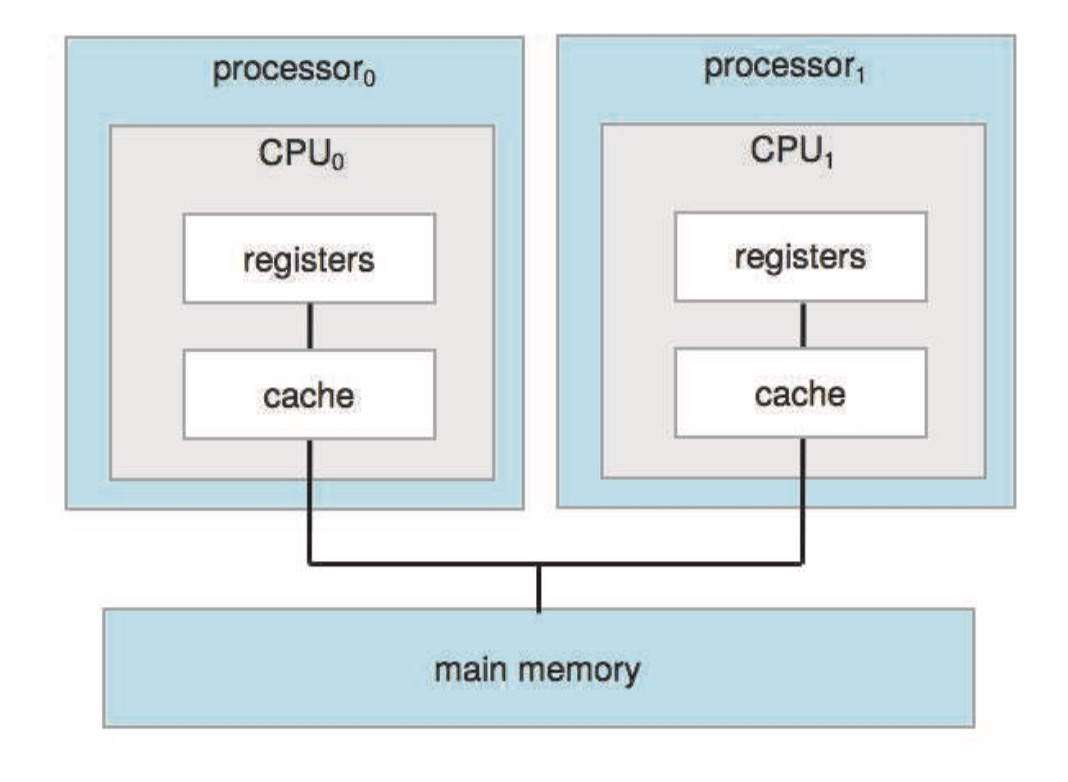
\includegraphics[width=0.6\textwidth]{figures/symmetric-multiprocessing-architecture.jpg}
            \caption{Symmetric \textit{multiprocessing} architecture}
            \label{fig:symmetric-multiprocessing-architecture}
        \end{figure}
    \item \textbf{Multiprocessor Advantages (Increased Throughput):} Primary advantages of multiprocessor systems is increased throughput. The speed-up ratio with \(N\) processors is not \(N\), however; it is less than \(N\) because there is overhead incurred and contention for shared resources when dealing with multiple processors.
    \item \textbf{Multicore Systems:} A computer system containing multiple cores on the same processor chip (figure \ref{fig:multicore-architecture}). Such systems can be more efficient than multiple chips with single cores because on-chip communication is faster than between-chip communication. Additionally, one chip with multiple cores uses significantly less power than multiple single-core chips, an issue especially important for mobile devices.
        \begin{figure}[ht]
            \centering
            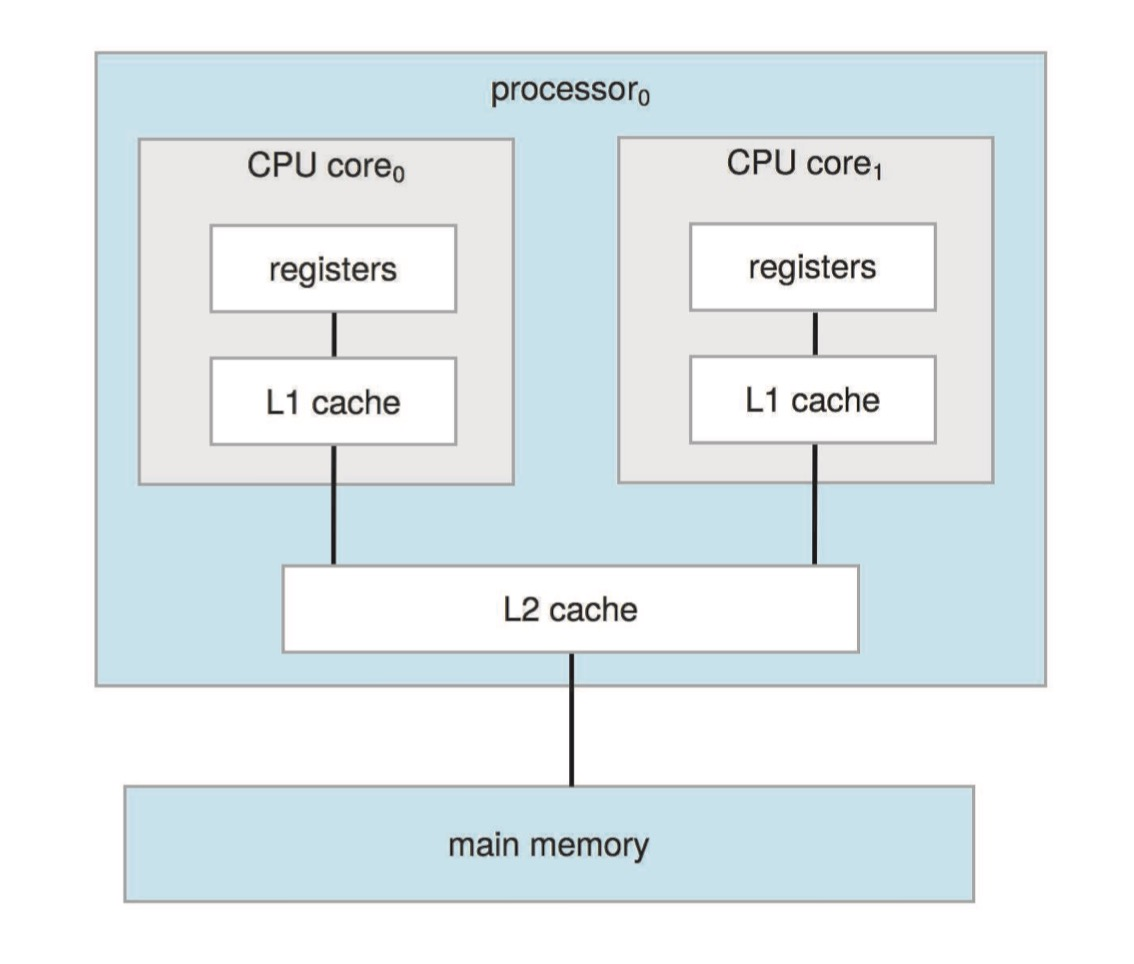
\includegraphics[width=0.6\textwidth]{figures/multicore-architecture.jpg}
            \caption{\textit{Multicore} architecture}
            \label{fig:multicore-architecture}
        \end{figure}
    \item \textbf{Multiprocessor Bottleneck:} Adding additional CPU's to a multiprocessor system increases computing power, but does not scale very well. Once too many CPU's are added, contention for the system bus becomes a bottleneck and performance begins to degrade.
    \item \textbf{Non-uniform Memory Access (NUMA):} To avoid bottleneck performance degradation arising from system bus contention, we can provide each CPU with its own local memory that is accessed via a small and fast local bus (figure \ref{fig:numa-architecture}). The CPU's are connected by a shared system interconnect, so that all CPU's share one physical address space. The advantage is that when a CPU accesses its local memory, not only is it fast, but there is also no contention over the system interconnect. Thus, NUMA systems can scale more effectively as more processors are added.
        \begin{figure}[ht]
            \centering
            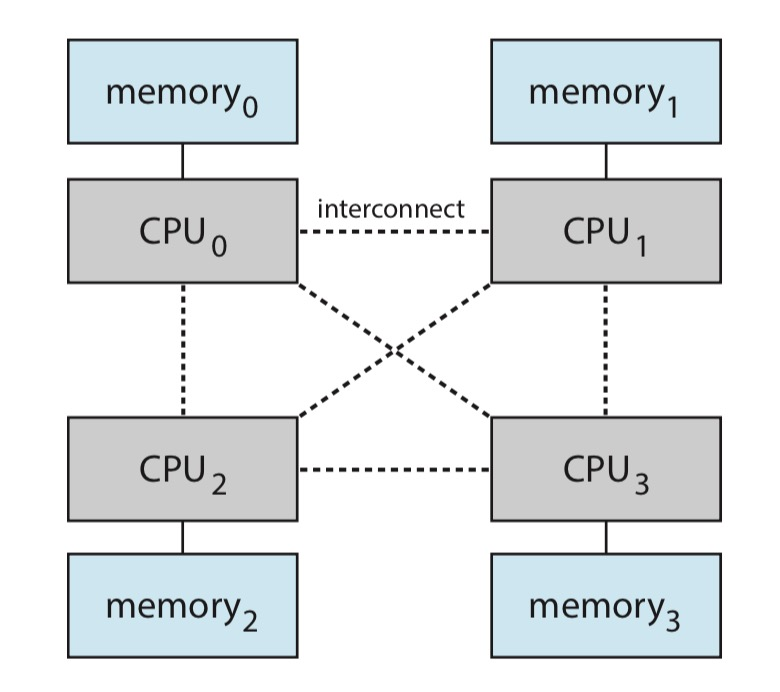
\includegraphics[width=0.4\textwidth]{figures/numa-architecture.jpg}
            \caption{NUMA architecture}
            \label{fig:numa-architecture}
        \end{figure}
    \item \textbf{NUMA Drawbacks (Increased Latency):} A potential drawback is increased latency when a CPU must access remote memory across the system interconnect (accessing the local memory of another CPU). OS's can minimize this NUMA penalty through careful CPU scheduling and memory management.
\end{itemize}

\section*{OS Concepts 1.4: Operating-System Operations}
\addcontentsline{toc}{section}{1.4: Operating-System Operations}

\begin{itemize}
    \item \textbf{Bootstrap Program:} The initial program that is run when a computer starts running for the first time. Typically a very simple program and stored in firmware. The program must know how to load the OS kernel into memory and start executing it.
    \item \textbf{System Daemons:} Services provided outside of the kernel that are loaded into memory at boot time, which run the entire time the kernel is running.
\end{itemize}

\subsection*{1.4.1: Multiprogramming and Multitasking}
\addcontentsline{toc}{subsection}{1.4.1: Multiprogramming and Multitasking}

\begin{itemize}
    \item \textbf{Multiprogramming:} Increase CPU utilization by organizing programs so that the CPU always has one to execute. Execute a process until it needs to wait on some task like I/O, then switch to another process. Keep switching between processes such that the CPU is never idle.
    \item \textbf{Process:} In a multiprogrammed system, a program in execution is termed a process.
    \item \textbf{Multitasking:} The logical extension of multiprogramming. In multitasking systems, the CPU executes multiple processes by switching among them incredibly frequently. This is how interactive I/O like keyboard input works: rather than letting the CPU sit idle in the time between the keystrokes of the user, the OS will rapidly switch to another process in the meantime.
\end{itemize}

\subsection*{1.4.2: Dual-Mode and Multimode Operation}
\addcontentsline{toc}{subsection}{1.4.2: Dual-Mode and Multimode Operation}

\begin{itemize}
    \item \textbf{Modes of Execution:} A properly designed OS must ensure that an incorrect (or malicious) program cannot cause other programs - or the OS itself - to execute incorrectly. To do this, we need to distinguish between the execution of OS code and user-defined code. Most computer systems provide hardware support that allows differentiation among various modes of execution.
    \item \textbf{User Mode and Kernel Mode:} At the very least, we need two separate modes of operation: user mode and kernel mode (also called supervisor mode, system mode, or privileged mode). A bit, called the mode bit, is added to the hardware of the computer to indicate the current mode: kernel (0) or user (1). Whenever the OS gains control of the computer, it is in kernel mode. The system always switches back to user mode before passing control to a user program. The concept of modes can be extended beyond two modes (e.g. the four protection rings in Intel processors).
    \item \textbf{Privileged Instructions:} Some machine instructions that may cause harm can only be executed in kernel mode. The instruction to switch to kernel mode is an example of a privileged instruction.
\end{itemize}

\subsection*{1.4.3: Timer}
\addcontentsline{toc}{subsection}{1.4.3: Timer}

\begin{itemize}
    \item \textbf{Timer:} We must ensure that the OS maintains control over the CPU: we allow user programs to execute, but they must eventually relinquish control to the OS (avoid situations like user program infinite loops or not calling system services and thus not returning control to the OS). To accomplish this, we can use a timer that is set to raise an interrupt after a specified amount of time. If the timer interrupts, control transfers automatically to the OS, which may treat the interrupt as a fatal error or may give the program more time. Instructions that modify the timer are clearly privileged.
\end{itemize}

\section*{OS Concepts 1.5: Resource Management}
\addcontentsline{toc}{section}{1.5: Resource Management}

The OS can be seen as a resource manager. The following are things that the OS must carefully manage in a computer system.

\subsection*{1.5.1: Process Management}
\addcontentsline{toc}{subsection}{1.5.1: Process Management}

\begin{itemize}
    \item \textbf{Program vs Process:} A program by itself is not a process. A program is a \textit{passive} entity, whereas a process is an \textit{active} entity. Remember that a process is just a program in execution, thus there can be multiple processes associated with the same program (and each is considered a separate execution sequence).
\end{itemize}

\subsection*{1.5.2: Memory Management}
\addcontentsline{toc}{subsection}{1.5.2: Memory Management}

\begin{itemize}
    \item \textbf{Memory Management:} The OS is responsible for keeping tack of which parts of memory are currently being used and which process is using them, allocating and deallocating memory, and deciding which processes (or parts of processes) and data to move into and out of memory.
\end{itemize}

\subsection*{1.5.3: File-System Management}
\addcontentsline{toc}{subsection}{1.5.3: File-System Management}

\begin{itemize}
    \item \textbf{File System:} The OS abstracts the physical properties of its storage devices to define a logical storage unit, the \textbf{file}. In other words, the OS implements the abstract concept of a file by managing mass storage media and the devices that control them.
\end{itemize}

\subsection*{1.5.4: Mass-Storage Management}
\addcontentsline{toc}{subsection}{1.5.4: Mass-Storage Management}

\begin{itemize}
    \item \textbf{Secondary Storage Management:} The proper management of secondary storage is critical to a computer system. The OS must take care of things such as mounting and unmounting, free-space management, storage allocation, disk scheduling, partitioning, and protection.
\end{itemize}

\subsection*{1.5.5: Cache Management}
\addcontentsline{toc}{subsection}{1.5.5: Cache Management}

\begin{itemize}
    \item \textbf{OS and Memory Hierarchy:} The OS is responsible for moving data between the different levels of the memory hierarchy that it has access to. The OS can only manipulate software-controlled caches, for instance transfer of data from disk to memory, while data transfer from CPU cache to registers is a hardware function.
    \item \textbf{Caches and Multitasking:} In a computing environment where only one process executes at a time, having the same data appear in multiple levels of the memory hierarchy is not an issue, since access to desired memory always will be to the copy at the highest level of the hierarchy. In a multitasking environment, however, extreme care must be taken to ensure that if several processes wish to access the same data, each of these processes obtains the most recently updated value of the data.
    \item \textbf{Caches and Multiprocessor Systems:} In a multiprocessing environment, not only do we need to make sure that processes access the most recenly updated value of the desired data (multitaking), but we now have CPUs that contain local caches in which data may esist simultaneously in several of these. We need to make sure that an update to the value of a given piece of data in one cache is immediately reflected in all other caches where this data resides. This issue if called \textit{cache conherency}, and is usually handled in hardware (below the OS level).
\end{itemize}

\subsection*{1.5.6: I/O System Management}
\addcontentsline{toc}{subsection}{1.5.6: I/O System Management}

\begin{itemize}
    \item \textbf{I/O Subsystem:} One of the purposes of an OS is to hide the peculiarities of specific hardware devices from the user. Often, these peculiarities are hidden from most of the OS itself by the I/O subsystem. Device drivers for specific hardware devices for instance are included in the I/O subsystem.
\end{itemize}

\section*{OS Concepts 1.7: Virtualization}
\addcontentsline{toc}{section}{1.7: Virtualization}

\begin{itemize}
    \item \textbf{Virtualization:} Virtualization allows us to abstract the hardware of a single computer (the CPU, memory, disk drives, etc.) into several different execution environments, creating the illusion that each separate environment is running on its own private computer. An OS that is natively compiled for a particular CPU architecture runs within another OS also native to that CPU.
    \item \textbf{Emulation:} Simulates computer hardware in software, typically used when the source CPU type is different from the target CPU type (e.g. Apple Rosetta when moving from PowerPC to x86). Usually much slower than native code.
\end{itemize}

\section*{OS Concepts 1.10: Computing Environments}
\addcontentsline{toc}{section}{1.10: Computing Environments}

\subsection*{1.10.4: Peer-to-Peer Computing}
\addcontentsline{toc}{subsection}{1.10.4: Peer-to-Peer Computing}

\begin{itemize}
    \item \textbf{Peer-to-Peer (P2P) Computing:} In this distributed computing model, clients and servers are not distinguished from each other. Each node in the system may act as either a client or a server, depending on whether it is requesting or providing a service. In traditional client-server systems, the server is a bottleneck; but in a P2P system, services can be provided by several nodes distributed throughout the network.
    \item \textbf{Centralized P2P:} When a node first joins a network, it registers its service with a centralized lookup service on the network. Any node desiring a specific service first contacts this centralized lookup service to determine which node provides the service. The remainder of the communication takes place between the client and the service provider.
    \item \textbf{Decentralized P2P:} A decentralized system uses no centralized lookup service. Instead, a peer acting as a client must discover what node provides a desired service by broadcasting a request for the service to all other nodes in the network. To support this approach, a \textit{discovery protocol} must be provided that allows peers to discover services provided by other peers in the network.
\end{itemize}

\section*{OS Concepts 2.6: Why Applications are OS Specific}
\addcontentsline{toc}{section}{2.6: Why Applications are OS Specific}

\begin{itemize}
    \item \textbf{Why Applications are OS Specific:} Each OS exposes different functionalities (system calls), so applications cannot expect to be able to use the same functions across varying OS's. Even if system calls were somehow uniform, other barriers would still pose a challenge: binary formats, varying CPU ISA's, system call discrepancies (specific operands and operand ordering, how to invoke syscalls, syscall result meanings, etc.).
    \item \textbf{How to Make Applications Cross Compatible Across OS's:}
    \begin{itemize}
        \item Write the application in an \textit{interpreted language} (e.g. Python or Ruby); performance typically suffers. and interpreter usually only offers a subset of the OS's features.
        \item Write the application in a language that includes a \textit{virtual machine} (e.g. Java). The JVM has been ported to many OS's, and in theory any Java app can run within the JVM wherever it's available. Usually have similar disadvantages as with interpreted languages.
        \item Use a language that compiles \textit{machine and OS specific binaries} (e.g. C++ or Rust), and simply port to each OS on which it will run. Standard API's like POSIX can make this process easier.
    \end{itemize}
\end{itemize}

\section*{OS Concepts 2.7: OS Design and Implementation}
\addcontentsline{toc}{section}{2.7: OS Design and Implementation}

\subsection*{2.7.1: Design Goals}
\addcontentsline{toc}{subsection}{2.7.1: Design Goals}

\begin{itemize}
    \item \textbf{OS Goals and Specifications:} The first problem in designing a system is to define goals and specifications. These requirements can, however, be divided into two basic groups: user goals and system goals.
\end{itemize}

\subsection*{2.7.2: Mechanisms and Policies}
\addcontentsline{toc}{subsection}{2.7.2: Mechanisms and Policies}

\begin{itemize}
    \item \textbf{Mechanisms and Policies:} An important principle is the separation of policy from mechanism. Mechanisms determine \textit{how} to do something; policies determine \textit{what} will be done. For instance, the standard Linux kernel has a specific CPU scheduling algorithm, which is a mechanism that supports a certain policy. However, anyone is free to modify or replace the scheduler to support a different policy.
\end{itemize}

\section*{OS Concepts 2.8: OS Structure}
\addcontentsline{toc}{section}{2.8: OS Structure}

\subsection*{2.8.1: Monolithic Structure}
\addcontentsline{toc}{subsection}{2.8.1: Monolithic Structure}

\begin{itemize}
    \item \textbf{Monolithic Structure:} A monolithic kernel places all of the functionality of the kernel into a single, static binary file that runs in a single address space. Everything below the system-call interface and above the physical hardware is the kernel, as seen in figure \ref{fig:monolithic-structure}. Typically difficult to implement and extend, but have good performance due to very little overhead in the syscall interface, and communication within the kernel is fast.
        \begin{figure}[ht]
            \centering
            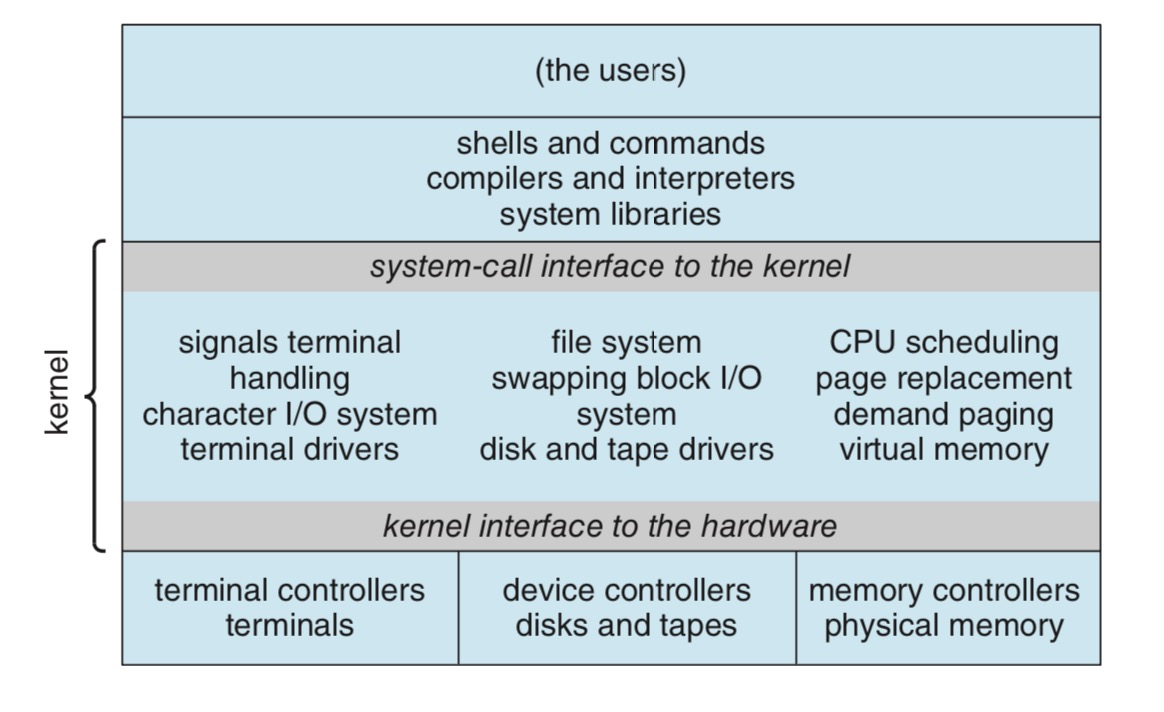
\includegraphics[width=0.7\textwidth]{figures/monolithic-structure.jpg}
            \caption{Traditional UNIX system structure (monolithic architecture)}
            \label{fig:monolithic-structure}
        \end{figure}
\end{itemize}

\subsection*{2.8.3: Microkernels}
\addcontentsline{toc}{subsection}{2.8.3: Microkernels}

\begin{itemize}
    \item \textbf{What is a Microkernel?} The microkernel approach structures the OS by removing all nonessential components from the kernel and implementing them as user-level programs that reside in separate address spaces, resulting in a smaller kernel, seen in figure \ref{fig:microkernel-structure}. There is little consensus on what services remain in the kernel, however, typically minimal process and memory management and a communication facility are provided. The main function of the microkernel is to provide communication between the client program and the various services also running in user space; communication is provided though message passing.
        \begin{figure}[ht]
            \centering
            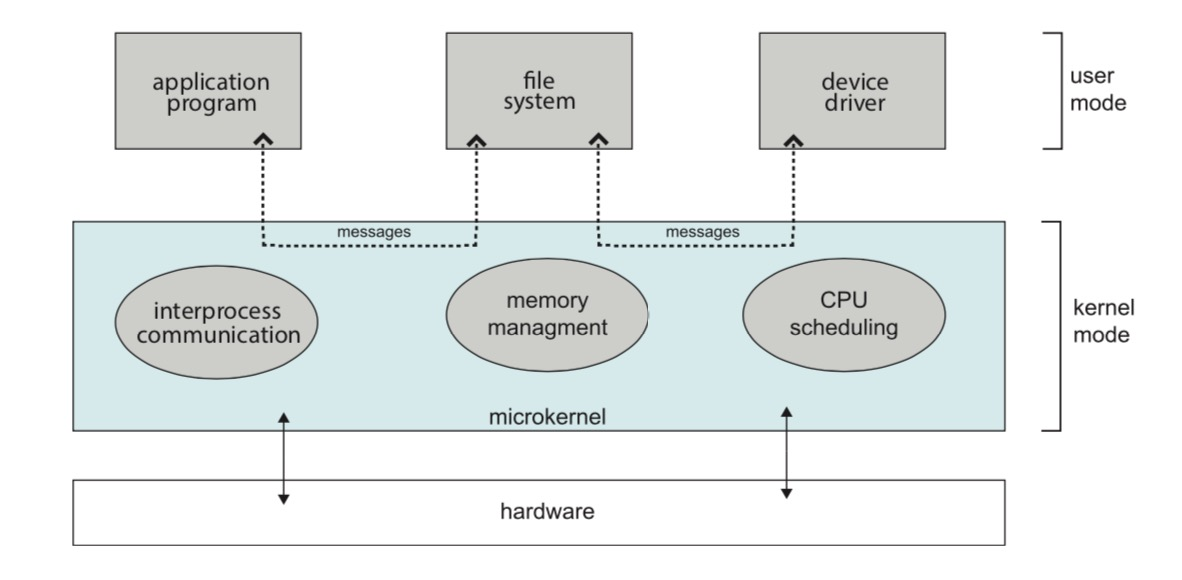
\includegraphics[width=0.8\textwidth]{figures/microkernel-structure.jpg}
            \caption{Architecture of a typical microkernel}
            \label{fig:microkernel-structure}
        \end{figure}
    \item \textbf{Microkernel Benefits:} The microkernel approach makes extending the OS easier, as all new services are added to user space and do not require modification of the kernel. When the kernel does have to be modified, the changes tend to be fewer as the kernel is smaller. It also makes porting the OS to different hardware easier and provides more security and reliability, as most services are running as user -rather than kernel- processes.
    \item \textbf{Microkernel Drawbacks:} Performance of microkernels can suffer due to increased system-function overhead. The overhead involved in copying messages and switching between processes has been the larged impediment to the groth of microkernel-based OS's.
\end{itemize}

\subsection*{2.8.4: Modules}
\addcontentsline{toc}{subsection}{2.8.4: Modules}

\begin{itemize}
    \item \textbf{Loadable Kernel Modules (LKMs):} Using LKMs, the kernel has a set of core components and can link in additional services via modules, either at boot time or during run time. The key idea is for the kernel to provide core services, while other services are implemented dynamically, as the kernel is running.
\end{itemize}

\section*{OS Concepts 2.9: Building and Booting an OS}
\addcontentsline{toc}{section}{2.9: Building and Booting an OS}

\subsection*{2.9.2: System Boot}
\addcontentsline{toc}{subsection}{2.9.2: System Boot}

\begin{itemize}
    \item \textbf{Booting OS:} When starting a computer system, how does the hardware know where the kernel is or how to load that kernel? This process of loading the kernel is known as booting the system. The boot process typically roughly follows as so:
    \begin{enumerate}
        \item A small piece of code known as the bootstrap program or boot loader locates the kernel
        \item The kernel is loaded into memory and started
        \item The kernel initializes the hardware
        \item The root file system is mounted
    \end{enumerate}
    \item \textbf{BIOS:} Some (typically older) computers use a multistage boot process: when the computer first powered on, a small boot loader located in nonvolatile firmware known as BIOS is run. This initial bootloader usually does nothing more than load a second boot lader, which is located at a fixed disk location called the boot block, which is then responsible for loading the OS into memory and begin execution.
    \item \textbf{UEFI:} More recent computers have replaced the BIOS-based boot process with UEFI (Unified Extensible Firmware Interface). The biggest difference is that UEFI is a single, complete boot manager and therefore is faster than the multistage BIOS boot process.
\end{itemize}

\section*{OS Concepts 3.1: Process Concept}
\addcontentsline{toc}{section}{3.1: Process Concept}

\subsection*{3.1.1: The Process}
\addcontentsline{toc}{subsection}{3.1.1: The Process}

\begin{itemize}
    \item \textbf{What is a process?} A process is a program in execution. A program becomes a process when an executable file is loaded into memory. Although two processes may be associated with the same program, they are nevertheless considered two separate esecution sequences.
    \item \textbf{What does a running process consist of?} The current activity of a process is represented by the value of the program counter and the contents of the processor's registers (the preservation of a processes memory address space depends on the memory management method of the OS).
    \item \textbf{What does the memory layout of a process look like?} The memory layout of a process is typically divided into multiple sections (figure \ref{fig:process-memory-layout}), the most important being:
        \begin{itemize}
            \item \textbf{Text} - the executable code
            \item \textbf{Data section} - global variables
            \item \textbf{Heap section} - memory that is dynamically allocated during program runtime
            \item \textbf{Stack section} - temporary data storage when invoking functions (such as function parameters, return addresses, and local variables)
        \end{itemize}
        \begin{figure}[ht]
            \centering
            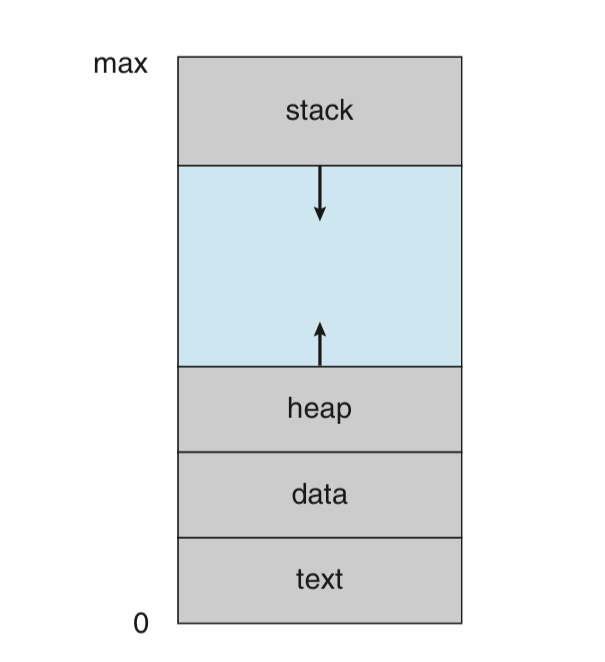
\includegraphics[width=0.4\textwidth]{figures/process-memory-layout.jpg}
            \caption{Memory layout of a process}
            \label{fig:process-memory-layout}
        \end{figure}
\end{itemize}

\subsection*{3.1.2: Process State}
\addcontentsline{toc}{subsection}{3.1.2: Process State}

\begin{itemize}
    \item \textbf{What are the different states a process can be in?} In general, a process may be in one of the following states (diagram in figure \ref{fig:process-states}):
    \begin{itemize}
        \item \textbf{New:} The process is being created.
        \item \textbf{Running:} Instructions are being executed.
        \item \textbf{Waiting:} The process is waiting for some event to occur (such as an I/O completion), it is blocked.
        \item \textbf{Ready:} The process is waiting to be assigned to a processor.
        \item \textbf{Terminated:} The process has finished execution.
    \end{itemize}
    \begin{figure}[ht]
        \centering
        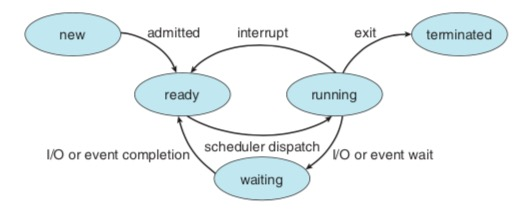
\includegraphics[width=0.7\textwidth]{figures/process-states.jpg}
        \caption{Diagram of process states}
        \label{fig:process-states}
    \end{figure}
\item \textbf{How many processes can be running on a processor core at any given time?} Only one process can be actively running (in the running state) on any processor core at any given time. Many processes may be in the ready or waiting state, however.
\end{itemize}

\subsection*{3.1.3: Process Control Block}
\addcontentsline{toc}{subsection}{3.1.3: Process Control Block}

\begin{itemize}
    \item \textbf{How is information about a process tracked by the OS?} The OS maintains information about each process in a data structure called the process control block (PCB), shown in figure \ref{fig:process-control-block}. Basically it contains all the necessary information required to start, or restart, a process, along with bookkeeping data. On systems that support threads, the PCB is expanded to include information for each thread.
    \begin{figure}[ht]
        \centering
        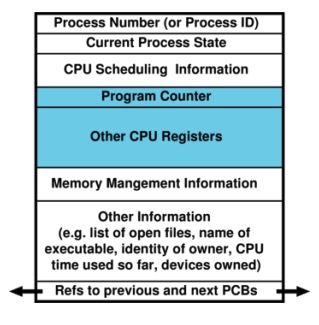
\includegraphics[width=0.4\textwidth]{figures/process-control-block.jpg}
        \caption{The process control block. The highlighted blue region is the machine environment during the time the process is actively in control of the CPU.}
        \label{fig:process-control-block}
    \end{figure}
\end{itemize}

\section*{OS Concepts 3.2: Process Scheduling}
\addcontentsline{toc}{section}{3.2: Process Scheduling}

\begin{itemize}
    \item \textbf{How are processes selected to be run?} To maximize CPU utilization by having some process running at all times and to support efficient multitasking by switching among processes frequently enough, the \textbf{process scheduler} is responsible for selecting an available process for program execution on a CPU core (balancing multiprogramming and time sharing). For a single core system there will never be more than one process running at a time, whereas a multicore system can run multiple processes at a time.
    \item \textbf{Degree of multiprogramming:} The number of processes currently in memory.
    \item \textbf{I/O Bound:} An I/O bound process is one whose speed is bound by the I/O (i.e. it doesn't matter if the CPU is blazing fast, the program speed will still be limited by how fast I/O completes).
    \item \textbf{CPU Bound:} A CPU bound process is one whose speed is limited by the speed of the CPU (i.e. it would go faster if the CPU could go faster).
\end{itemize}

\subsection*{3.2.1: Scheduling Queues}
\addcontentsline{toc}{subsection}{3.2.1: Scheduling Queues}

\begin{itemize}
    \item \textbf{What happens to a process when it first enters the system?} As processes enter the system, they are put into a \textbf{ready queue}, where they have the "ready" state and waiting to be executed (dispatched) on a CPU's core. This queue is typically implemented as a linked list, containg pointers to PCB structures. See figure \ref{fig:queueing-diagram}.
    \item \textbf{What happesn to a process when it is waiting?} A process in a waiting state (waiting for I/O, time slice expired, etc.) is put into the \textbf{wait queue}. See figure \ref{fig:queueing-diagram}.
    \begin{figure}[ht]
        \centering
        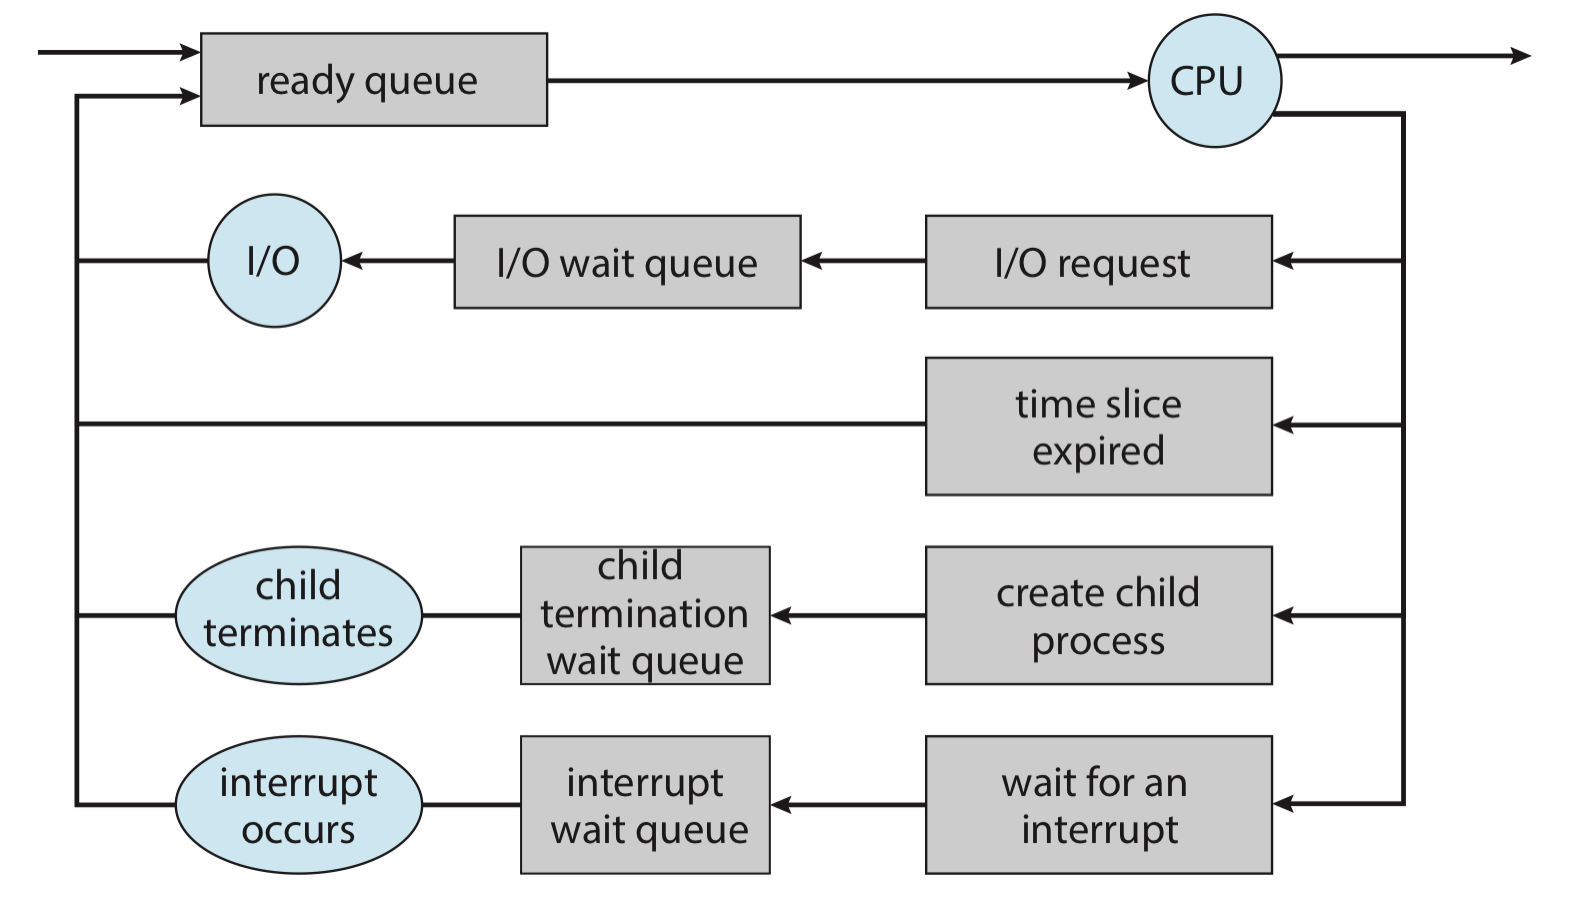
\includegraphics[width=0.7\textwidth]{figures/queueing-diagram.jpg}
        \caption{Representation of process scheduling}
        \label{fig:queueing-diagram}
    \end{figure}
\end{itemize}

\subsection*{3.2.3: Context Switch}
\addcontentsline{toc}{subsection}{3.2.3: Context Switch}

\begin{itemize}
    \item \textbf{What happens when the CPU needs to switch to a different process?} When switching to another process, whether that be because of an interrupt, time slice expired, or any another reason, the current context of the running process on the CPU core needs to be saved (state save). The context is represented in the PCB of the context. The CPU then needs to restore the context of the other process it wishes to switch to (state restore). This process is known as a \textbf{context switch}.
    \item \textbf{What are the performance implications of a context switch?} A context switch is pure overhead. The system does no useful work while switching processes. A typical context switch takes several microseconds, but is highly dependent on the hardware the OS is running on.
\end{itemize}

\section*{OS Concepts 3.3: Operations on Processes}
\addcontentsline{toc}{section}{3.3: Operations on Processes}

\subsection*{3.3.1: Process Creation}
\addcontentsline{toc}{subsection}{3.3.1: Process Creation}

\begin{itemize}
    \item \textbf{How are processes created?} During the course of execution, a process may create several new processes. The creating process is called the \textbf{parent} process, and the new processes it has created are called the \textbf{children} of that process. Each of these new processes may in turn create other processes, forming a hierarchical tree.
    \item \textbf{How are processes identified?} Most OS's use unique process identifiers (PID, typically an integer) to identify processes. The PID provides a unique value for each process in the system.
    \item \textbf{What is the ultimate parent process (chicken and egg problem)?} In a Linux OS, the \texttt{systemd} process (which always has a PID of 1) serves as the root process for all user processes. It is the first user process created when the system boots. Once the system has booted, the \texttt{systemd} process creates processes that provide additional services, like an \texttt{ssh} server or a login server.
    \item \textbf{How are resources and initialization of processes handled?} In general, child processes require resources (CPU time, memory resources, I/O devices, files) to accomplish its task. There are several options how this is handled:
        \begin{itemize}
            \item Parent and child share all resources
            \item Children share subset of parent's resources
            \item Parent and child share no resources
        \end{itemize}
    \item \textbf{How are parent and child processes executed?} The parent process may continue to execute \textbf{concurrently} with its children, or it may \textbf{wait} until some or all of its children have terminated.
    \item \textbf{What are the address-space possibilities for the new child process?} The child process is a \textbf{duplicate} of the parent process (it has the same program and data as input), or the child process has a program \textbf{loaded} into it.
    \item \textbf{What does process creation on a UNIX system typically look like?} Diagram in figure \ref{fig:unix-process-creation}. The parent process calls \texttt{fork()}, at which both the parent and child process continue execution (of the same program). After a \texttt{fork()} call, one of the processes typically uses the \texttt{exec()} system call to replace the process's memory space with a new program. The parent can then create more children; or, if it has nothing else to do while the child runs, it can issue a \texttt{wait()} system call to move itself off the ready queue until the termination of the child.
        \begin{figure}[ht]
            \centering
            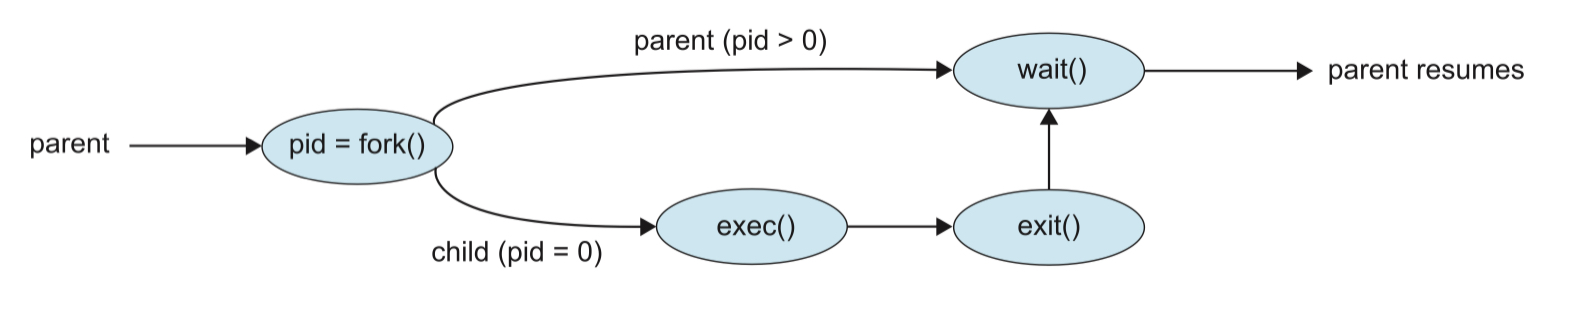
\includegraphics[width=0.8\textwidth]{figures/unix-process-creation.jpg}
            \caption{Representation of typical process creation on a UNIX system}
            \label{fig:unix-process-creation}
        \end{figure}
\end{itemize}

\subsection*{3.3.2: Process Termination}
\addcontentsline{toc}{subsection}{3.3.2: Process Termination}

\begin{itemize}
    \item \textbf{What happens when a process is terminated?} When a process is terminated, all the resources of the process (including virtual and physical memory, open files, and I/O buffers) are deallocated and reclaimed by the OS.
    \item \textbf{Under what situations can a process be terminated?} A process can be terminated under three circumstances:
        \begin{itemize}
            \item Process executes last statement and asks the OS to delete it (\texttt{exit()} syscall, either called explicitly or implicitly by C run-time library)
            \item Process performs an illegal operation (e.g. access memory it is not authorized for or execute a privileged instruction)
            \item Parent may terminate child process (child process exceeding resource usage, task assigned to child no longer required, or parent is exiting and OS uses cascading termination - if a process terminates so must all its children)
        \end{itemize}
\end{itemize}

\section*{OS Concepts 3.4: Interprocess Communication}
\addcontentsline{toc}{section}{3.4: Interprocess Communication}

\begin{itemize}
    \item \textbf{How do processes communicate with each other?} Using interprocess communication (IPC): implemented using either shared memory or message passing.
\end{itemize}

\section*{OS Concepts 3.5: IPC in Shared-Memory Systems}
\addcontentsline{toc}{section}{3.5: IPC in Shared-Memory Systems}

\begin{itemize}
    \item \textbf{How does shared memory IPC work?} Normally, the OS tries to prevent processes from accessing memory of other processes. Shared memory IPC requires that two or more processes agree to remove this restriction, so that they can then exchange information by reading and writing data in the shared memory areas.
    \item \textbf{How is shared memory access coordinated among processes?} Processes must themselves ensure that they are not writing to the same location simultaneously.
\end{itemize}

\section*{OS Concepts 3.6: IPC in Message-Passing Systems}
\addcontentsline{toc}{section}{3.6: IPC in Message-Passing Systems}

\begin{itemize}
    \item \textbf{What is message passing IPC?} Message passing provides a mechanism to allow processes to communicate and to synchronize their actions without sharing the same address space (particularly useful in distributed environments). Message passing may be either \textbf{blocking} or \textbf{nonblocking} (also known as synchronous or asynchronous).
\end{itemize}

\section*{OS Concepts 3.7: Examples of IPC Systems}
\addcontentsline{toc}{section}{3.7: Examples of IPC Systems}

\subsection*{3.7.4: Pipes}
\addcontentsline{toc}{subsection}{3.7.4: Pipes}

\subsubsection*{3.7.4.1: Ordinary Pipes}
\addcontentsline{toc}{subsubsection}{3.7.4.1: Ordinary Pipes}

\begin{itemize}
    \item \textbf{How do ordinary pipes work for IPC?} Ordinary (in contrast to named) pipes allow two processes to coomunicate in standard producer-consumer fashion: the producer writes to the write end of the pipe, and the consumer reads from the read end of the pipe. As a result, ordinary pipes are unidirectional (one-way communication), and bidirectional communication requires two pipes.
    \item \textbf{What processes can access an ordinary pipe?} On UNIX systems, ordinary pipes cannot be accessed from outside the process that created it. Typically, a parent process creates a pipe and uses it to communicate with a child process it created using \texttt{fork()}. In UNIX systems a child process inherits open files from its parent, hence why it is allowed to access the pipe. This also implies that ordinary pipes can only be used for communication between processes on the same machine.
\end{itemize}

\subsubsection*{3.7.4.2: Named Pipes}
\addcontentsline{toc}{subsubsection}{3.7.4.2: Named Pipes}

\begin{itemize}
    \item \textbf{What is difference between ordinary and named pipes?} Named pipes provide bidrectional communication, and do not require a parent-child process relationship. Once a named pipe is established, sefveral processes can use it for communication. Named pipes also continue to exist after communicating processes have finished, and must explicitly be deleted.
\end{itemize}

\section*{OS Concepts 4.1: Threads Overview}
\addcontentsline{toc}{section}{4.1: Threads Overview}

\begin{itemize}
    \item \textbf{What are threads?} A thread is a basic unit of CPU utilization. Processes can have multiple threads of control to perform more than one task at a time (threads exist as subsets of a process).
    \item \textbf{What is a thread comprised of?} A thread is comprised of a thread ID, a program counter (PC), a register set. and a stack.
    \item \textbf{What parts of a process do threads share?} Threads technically share everything belonging to a process, but each thread has it's own independent stack (and of course corresponding registers and a program counter, and possibly thread local storage if supported). Basically each thread contains its own state. Figure \ref{fig:thread-process} shows a rough visualization of how threads operate in the context of processes. Figure \ref{fig:thread-memory-layout} shows how multiple threads are laid out in the memory of a process.
        \begin{figure}[ht]
            \centering
            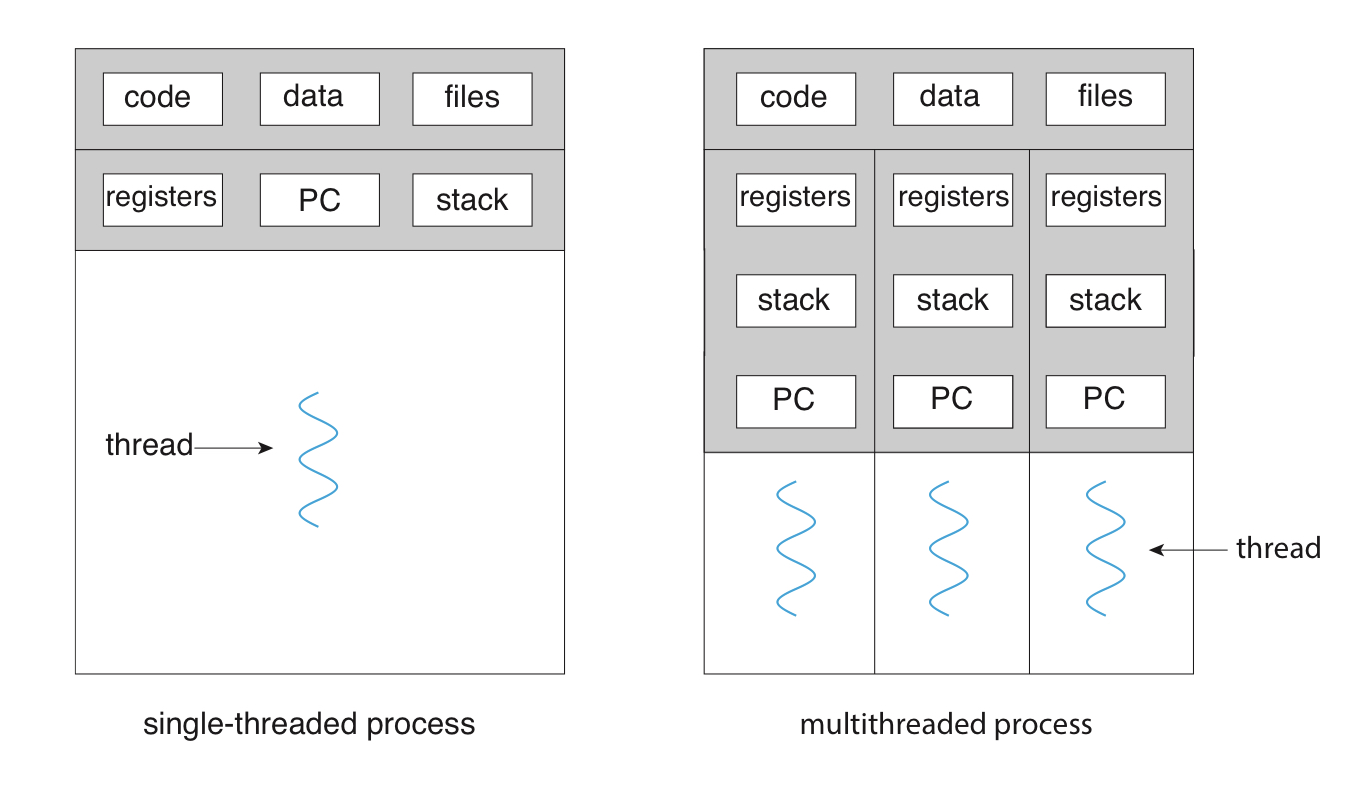
\includegraphics[width=0.8\textwidth]{figures/thread-process.jpg}
            \caption{Rough visualization of single vs multithreaded processes}
            \label{fig:thread-process}
        \end{figure}
        \begin{figure}[ht]
            \centering
            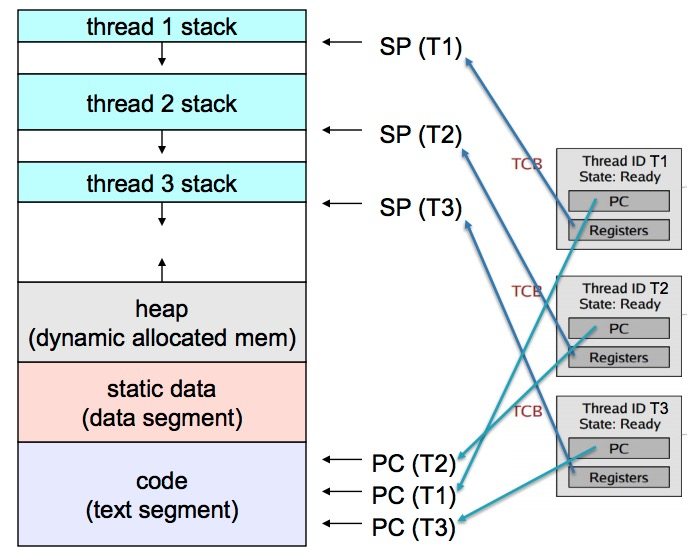
\includegraphics[width=0.6\textwidth]{figures/thread-memory-layout.jpg}
            \caption{Memory layout of a process with multiple threads. Stack pointers and program counters are tracked in the respective thread control blocks (TCB)}
            \label{fig:thread-memory-layout}
        \end{figure}
    \item \textbf{What is the high level difference between threads and processes?} Processes help organize two independent concepts in computing: resource grouping and execution. Resources (program text, data, open files, child processes, etc.) are grouped into a single process so that they can be managed easily. The other concept of a process is a thread of execution. Threads have program counters keeping track of which instructions to execute next, registers to hold its current working variables, and its own stack. Threads only operate in the context of processes. Processes are used to group resources together, while threads are entities scheduled for execution on the CPU.
    \item \textbf{Why might one want to use threads instead of processes?} Process creation is time consuming and resource intensive: it is generally more efficient to use one process that contains multiple threads. It makes particular sense to use threads when multiple tasks need to be performed at the same time using the same resources.
\end{itemize}

\section*{OS Concepts 4.2: Multicore Programming}
\addcontentsline{toc}{section}{4.2: Multicore Programming}

\begin{itemize}
    \item \textbf{What is multicore programming?} With the advent of multicore computer systems, multithreading provides a mechansim for more efficient use of thse multiple computing cores and improved concurrency.
    \item \textbf{What is the difference between concurrency and parallelism?} Consider an application with four threads. On a system with a single computing core, concurrency merely means that the execution of the threads will be interleaved over time (figure \ref{fig:concurrent-execution}). On a system with multiple cores, however, concurrency means that some threads can run in parallel, because the system can assign a separate thread to each core (figure \ref{fig:parallel-execution}). Thus, it is possible to have concurrency without parallelism.
        \begin{figure}[ht]
            \centering
            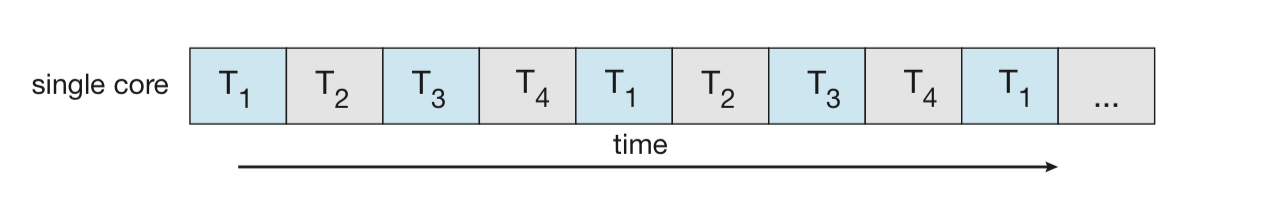
\includegraphics[width=0.8\textwidth]{figures/concurrent-execution.jpg}
            \caption{Concurrent execution on a single core system}
            \label{fig:concurrent-execution}
        \end{figure}
        \begin{figure}[ht]
            \centering
            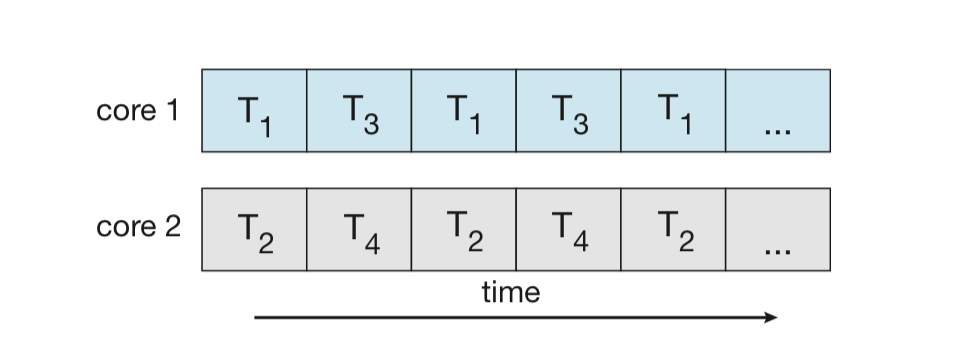
\includegraphics[width=0.6\textwidth]{figures/parallel-execution.jpg}
            \caption{Parallel execution on a multicore system}
            \label{fig:parallel-execution}
        \end{figure}
    \item \textbf{Concurrency:} Multiple threads making progress.
    \item \textbf{Parallelism} Multiple threads making progress \textit{simultaneously}.
    \item \textbf{What are the two types of parallelism?}
        \begin{itemize}
            \item \textbf{Data Parallelism:} Data parallelism focuses on distributing \textit{subsets} of the \textit{same data} across multiple computing cores and \textit{performing the same operation} on each core.
            \item \textbf{Task Parallelism:} Distributing not data but \textit{tasks} (threads) across multiple computing cores. Each thread is performing a \textit{unique operation}.
        \end{itemize}
    \item \textbf{Amdahl's Law:} The main idea behind Amdahl's law is that when we speed up one part of a system, the effect on the overall system performance depends on both what proportion of the overall system this part was and how much it sped up. We can interpret this in the context of multicore programming if we consider parallel components of a program being sped by up the number of processor cores \(N\). The key takeaway is that to significantly speed up an entire system, we must improve the speed of a very large fraction of the overall system. Derivation taken from CS:APP p22.
        \begin{itemize}
            \item \textbf{Derivation:} Consider a system in which executing some application requires time \(T_{\text{old}}\). Suppose some part of the system requires a fraction \(\alpha\) of this time, and that we improve its performance by a factor of \(k\). That is, the component originally required time \(\alpha T_{\text{old}}\), and now it requires time \((\alpha T_{\text{old}}) / k\). The overall execution time would thus be
                \begin{align*}
                    T_{\text{new}} & = (1 - \alpha) T_{\text{old}} + (\alpha T_{\text{old}}) / k \\
                                   & = T_{\text{old}} [(1 - \alpha) + \alpha / k]
                \end{align*}
                From this, we can compute the speedup \(S = T_{\text{old}} / T_{\text{new}}\) as
                \[S = \frac{1}{(1 - \alpha) + \alpha / k}\]
            \item \textbf{When N approaches infinity:} If the speedup \(k = N\) (number of processor cores in multicore context) approaches infinity, the speedup converges to \(\frac{1}{(1 - \alpha)}\). If two thirds of a program must be performed serially (parallel portion \(\alpha = 1/3\)), then the maximum speedup is 1.5 times, regardless of the number or processing cores \(N\) we add. It pays to be aware of exactly how much a program can really be sped up using parallelism (not much point if much of it needs to be done serially).
        \end{itemize}
\end{itemize}

\section*{OS Concepts 4.3: Multithreading Models}
\addcontentsline{toc}{section}{4.3: Multithreading Models}

\begin{itemize}
    \item \textbf{What is the difference between user and kernel threads?} User threads are implemented in userspace and managed without knowledge of the kernel (and neither does the kernel know about the user threads). Kernel threads are managed directly by the OS. User threads need to eventually map down somehow to kernel threads (important to take advantage of multicore systems, as user threads alone do not inherently support parallelism), different such multithreading models. Typically slightly more overhead when switching between kernel threads (user theads do not need to dip down to the kernel at all).
    \item \textbf{Many to One Model:} The many to one model maps many user level threads to one kernel thread (figure \ref{fig:many-to-one}). Essentially all the kernel sees is a single process, the threads are managed by a user-space thread library. Since this thread management is done by the thread library in user-space, it is very efficient (does not need to dip down into kernel, switching between kernel theads invoke expensive context switch costs). However, the entire process will block if a thread makes a blocking system call (again, because all the kernel sees is a single process). Also, since only one thread can access the kernel at a time, multiple threads are unable to run in parallel on multicore systems.
        \begin{figure}[ht]
            \centering
            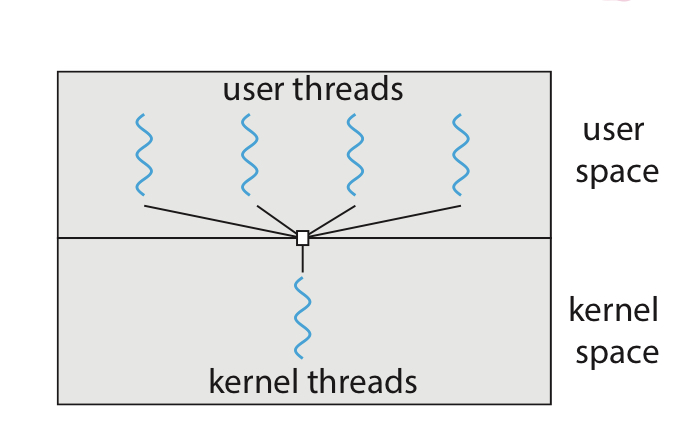
\includegraphics[width=0.4\textwidth]{figures/many-to-one.jpg}
            \caption{Many to one threading model}
            \label{fig:many-to-one}
        \end{figure}
    \item \textbf{One to One Model:} The one to one model maps each user thread to a kernel thread (figure \ref{fig:one-to-one}). It provides more concurrency than the many to one model by allowing another thread to run when a thread makes a blocking system call, as the kernel is responsible for managing these threads at the end of the day. Also allows multiple threads to run in \textbf{parallel} on multiprocessors. The only drawback to this model is that there is slightly more overhead involved with creating a kernel thread than just a pure user thread.
        \begin{figure}[ht]
            \centering
            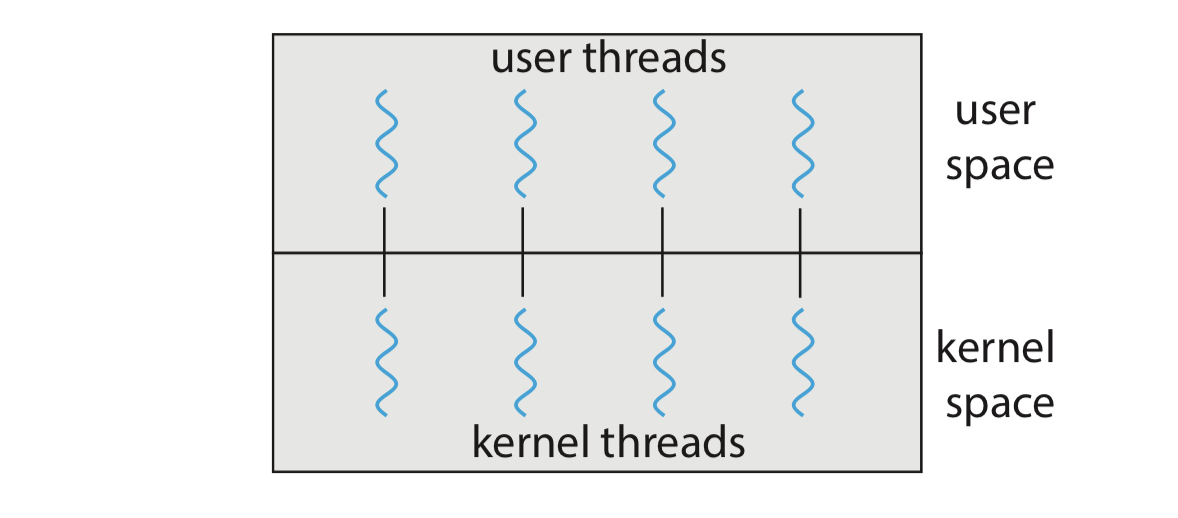
\includegraphics[width=0.5\textwidth]{figures/one-to-one.jpg}
            \caption{One to one threading model}
            \label{fig:one-to-one}
        \end{figure}
    \item \textbf{Many to Many (M:N) Model:} The M:N model \textit{multiplexes} \(M\) user level threads to \(N\) kernel threads, where \(M \geq N\) (figure \ref{fig:many-to-many}). In this model, the developer may create as many user theads as necessary, and the corresponding kernel threads can run in parallel on a multiprocessor. Also, when a thread performs a blocking system call, the kernel can simply schedule another thread for execution. Complex to implement, efficient performance requires extensive coordination between the userspace scheduler and the kernel scheduler.
        \begin{figure}[ht]
            \centering
            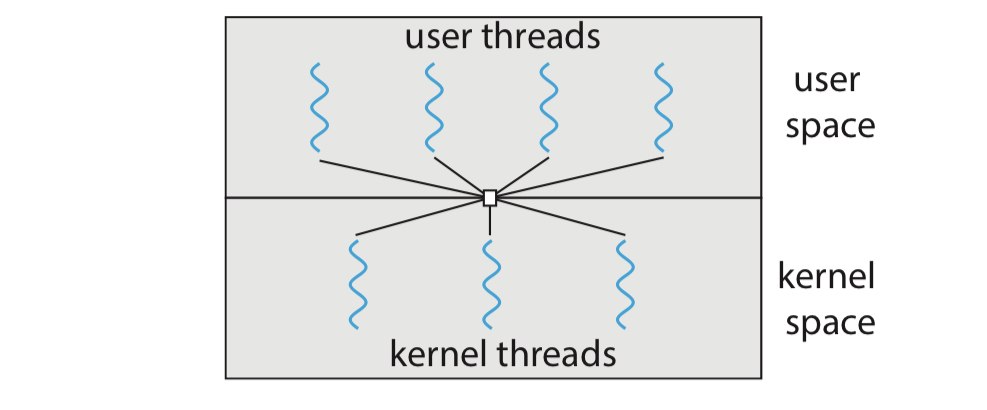
\includegraphics[width=0.5\textwidth]{figures/many-to-many.jpg}
            \caption{Many to many threading model}
            \label{fig:many-to-many}
        \end{figure}
\end{itemize}

\section*{OS Concepts 4.4: Thread Libraries}
\addcontentsline{toc}{section}{4.4: Thread Libraries}

\begin{itemize}
    \item \textbf{What are the two general strategies for creating multiple threads:} Asynchronous threading and synchronous threading.
    \item \textbf{Asynchronous Threading:} With asynchronous threading, once the parent creates a child thread, the parent resumes its execution, so that the parent and child execute concurrently and independently of on another.
    \item \textbf{Synchronous Threading:} With synchronous threading, the parent thread creates one or more children and then must wait for all of its children to terminate before it resumes. The threads created by the parent perform work concurrently, but the parent cannot continue until this work has been completed.
\end{itemize}

\section*{OS Concepts 4.5: Implicit Threading}
\addcontentsline{toc}{section}{4.5: Implicit Threading}

\begin{itemize}
    \item \textbf{What is implicit threading?} Implicit threading is basically transferring the responsibility of manually managing low level threads from developers to compilers and run-time libraries. Essentially, developers identify \textit{tasks} that they wish to execute concurrently, and these compilers and libraries do the grunt work of managing threads.
    \item \textbf{What are the benefits of using thread pools?} Thead pools offer these benefits:
        \begin{itemize}
            \item \textbf{Avoiding thread creation overhead:} Servicing a thread with an existing thread is often faster than waiting to create a thread.
            \item \textbf{Enforcing an upper bound to the number of threads:} A thread pool limits the number of threads that exist at any one point, important on systems that cannot support a large number of concurrent threads.
            \item \textbf{Moving from thread based to task based concurrency approach:} By using a thread pool, we can separate the idea of executing a task concurrently from the mechanics of creating such a task (threading). Basically lean on compilers and libraries to do threading grunt work (e.g. rayon and TBB).
        \end{itemize}
    \item \textbf{How do thread pools work?} The general idea behind a thread pool is to create a number of threads at start-up and place them into a pool, where they sit and wait for work. Users can submit task requests, and if there is an available thread in the pool, it is awakened, and the request serviced immediately. If the pool contains no available thread, the task is queued until one becomes free. Once a thread completes its service, it returns to the pool and awaits more work.
    \item \textbf{How do we determine the number of threads in a thread pool?} The number of threads in a pool can be heuristically set based on factors such as the number of CPUs, the amount of physical memory, and the expected number of concurrent client requests. More sophisticated thread pools can dynamically adjust the number of threads according to usage patterns (e.g. Grand Central Dispatch: makes pool smaller when system load is low, thereby consuming less memory).
\end{itemize}

\section*{OS Concepts 4.6: Threading Issues}
\addcontentsline{toc}{section}{4.6: Threading Issues}

\subsection*{4.6.1: The \texttt{fork()} and \texttt{exec()} System Calls}
\addcontentsline{toc}{subsection}{4.6.1: The \texttt{fork()} and \texttt{exec()} System Calls}

\begin{itemize}
    \item \textbf{How do the semantics of \texttt{fork()} change in a multithreaded program?} If one thread calls \texttt{fork()}, does the new process duplicate all threads, or is the new process single-threaded? Some UNIX systems have chosen to have two versions of \texttt{fork()}, one that duplicates all threads and another that duplicates only the thread that invoked the \texttt{fork()} system call.
    \item \textbf{How do the semantics of \texttt{exec()} change in a multithreaded program?} If a thread invokes \texttt{exec()}, the program specified in the parameter to \texttt{exec()} will replace the entire process - including all threads.
    \item \textbf{Which version of \texttt{fork()} to call in a multithreaded program?} If \texttt{exec()} is called immediately after forking, then duplicating all threads is unnecessary, as the new program specifiedto \texttt{exec()} will replace the whole process anyways.
\end{itemize}

\subsection*{4.6.2: Signal Handling}
\addcontentsline{toc}{subsection}{4.6.2: Signal Handling}

\begin{itemize}
    \item \textbf{What is a signal (in UNIX systems)?} A signal is used in UNIX systems to notify a process that a particular event has occurred, and may be received either synchronously or asynchronously. Synchronous signals are delivered to the same process that performed the operation that caused the signal (examples: illegal memory access and division by 0). When a signal is generated by an external event to a running process, that process receives the signal asynchronously (examples: terminated process with CTRL-C and having a timer expire).
    \item \textbf{How are signals handled?} Every signal has a default signal handler that the kernel runs, but can be overridden by user-defined signal handlers.
    \item \textbf{How are signals delivered to processes?} By using the UNIX function \texttt{kill()}.
    \item \textbf{How are signals delivered to multithreaded programs?} Synchronous signals are sent to the thread that caused the signal, and not to other threads in the process. Asynchronous signals are typically delivered only to the first thread found that is not blocking it (theads can choose which signals to accept and which to block).
\end{itemize}

\subsection*{4.6.3: Thread Cancellation}
\addcontentsline{toc}{subsection}{4.6.3: Thread Cancellation}

\begin{itemize}
    \item \textbf{What is thread cancellation?} Terminating a thread before it has completed.
    \item \textbf{What are the two types of thread cancellation?}
        \begin{itemize}
            \item \textbf{Asynchronous Cancellation:} One thread immediately terminates the target thread to be cancelled. This is troublesome when threads are cancelled in situations where resources have been allocated to these threads, or when a thread is cancelled in the midst of updating data shared with other threads.
            \item \textbf{Deferred Cancellation:} The target thread periodically checks whether it should terminate, allowing it to terminate itself in an orderly fashion (clean up and release resources).
        \end{itemize}
\end{itemize}

\subsection*{4.6.5: Scheduler Activations}
\addcontentsline{toc}{subsection}{4.6.5: Scheduler Activations}

\begin{itemize}
    \item \textbf{How are M:N theading models typically implemented (high level)?} Such systems usually place an intermediate data structure between the user and the kernel theads, typically known as a \textbf{lightweight process} (LWP). To the user-thread library, the LWP appears to be a virtual processor on which the application can schedule a user thread to run. Each LWP is attached to a kernel thread, and the kernel threads are scheduled by the OS to run on physical processors. If a kernel thread blocks (such as when waiting for I/O to complete), the LWP and the corresponding user-level threads attached to the LWP block as well. This is an issue when many concurrent blocking system calls are performed: if five I/O requests are made but only four LWPs are available, the firth request must wait for one of the four LWPs to return from the kernel before executing.
\end{itemize}

\section*{OS Concepts 4.7: OS Thread Examples}
\addcontentsline{toc}{section}{4.7: OS Thread Examples}

\begin{itemize}
    \item \textbf{How are threads and processes created on Linux?} Linux does not distinguish between processes and threads. Linux instead uses the term \textbf{task} - rather than process or thread when referring to a flow of control within a program. The Linux \texttt{clone()} system call provides the ability to create such tasks. The arguments passed to \texttt{clone()} specify the amount of data shared between parent and child tasks, thus making tasks behave more like processes or threads. The \texttt{fork()} system call on Linux is typically implemented using \texttt{clone()}.
\end{itemize}

\section*{OS Concepts 5.1: CPU Scheduling Basic Concepts}
\addcontentsline{toc}{section}{5.1: CPU Scheduling Basic Concepts}

\begin{itemize}
    \item \textbf{What is the motivation for CPU schduling?} In a system with a single CPU core, only one process can run at a time. This means if this single process is in control of the CPU and is waiting for some I/O request, the CPU is basically sitting doing nothing (which is a waste). With multiprogramming, several processes are kept in memory at a time, and we can swap a new process to do useful work while our original process is waiting for its I/O request to complete. This process of swapping out the tasks the CPU is currently executing is the realm of CPU scheduling.
    \item \textbf{What is the CPU-IO Burst Cycle?} Process execution consist of a cycle of CPU execution and then waiting for I/O (CPU burst and then I/O burst). This cycle is called the CPU-IO burst cycle; processes can be in one of the two states. Processes typically have a large amount of short CPU bursts and a small number of long CPU bursts. This frequency curve is shown in figure \ref{fig:cpu-io-burst}.
        \begin{figure}[ht]
            \centering
            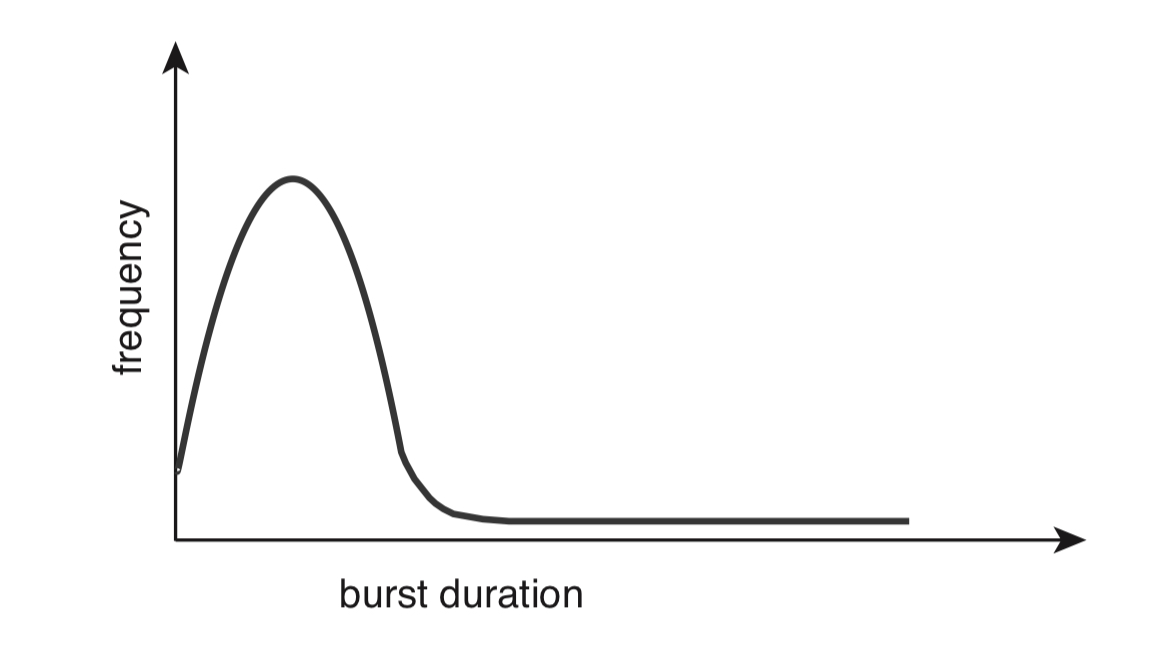
\includegraphics[width=0.7\textwidth]{figures/cpu-io-burst.jpg}
            \caption{Histogram of CPU burst durations}
            \label{fig:cpu-io-burst}
        \end{figure}
    \item \textbf{CPU Bound:} CPU bound processes are when the rate of progress for the process is limited by the actual speed of the CPU. The process would go faster with a faster CPU. The opposite of being I/O bound.
    \item \textbf{I/O Bound:}  I/O bound processes are when the rate of progress for the process is limited by the speed of the I/O it performs. A faster CPU would not help, only faster I/O completion times would cause the process to proceed faster. The process sits around doing nothing and waiting for I/O to complete (memory wall big issue, disparity between CPU and memory speeds).
    \item \textbf{What has the responsibility of choosing which process to execute on the CPU?} Whenever the CPU becomes idle, the OS must select one of the processes in the ready queue to be executed (not this is not necessarily a FIFO queue, various scheduling algorithms have different implementations). This selection process is carried out by the \textbf{CPU scheduler}, which selectrs a process from the processes in memory that are ready to execute (in the ready queue) and allocates the CPU to that process. The items in the queues are generally process control blocks (PCBs) of the processes (or TCBs for threads? IDK not sure).
    \item \textbf{Under what circumstances can CPU scheduling decisions take place?} CPU scheduling decisions may take place under the following four circumstances:
        \begin{enumerate}
            \item (Running \(\rightarrow\) Waiting) When a process switches from the running state to the waiting state (e.g. when requesting I/O or willingly switching to the waiting state like calling \texttt{wait()} for the termination of a child process)
            \item (Running \(\rightarrow\) Ready) When a process switches from the running state to the ready state (e.g. when an interrupt occurs)
            \item (Waiting \(\rightarrow\) Ready) When a process switches from the waiting state to the ready state (e.g. at completion of I/O)
            \item (Running \(\rightarrow\) Terminated) When a process terminates
        \end{enumerate}
    \item \textbf{Preemptive vs Cooperative Scheduling:} In situations 1 and 4 above, there is no choice in terms of scheduling: a new process \textit{must} be selected for execution. There is a choice, however, for situations 2 and 3. When scheduling takes place only under situations 1 and 4, scheduling is considered to be cooperative (process willingly gives up control): the process keeps control of the CPU until it releases it either by switching to the waiting state (situation 1) or by terminating (situation 4). When scheduling also occurs in situations 2 and 3 (in both situations the process is ready to continue execution by being in the ready state), scheduling is considered to be preemptive: the process could keep on running and keep control of the CPU, but instead is kicked off the CPU by the OS. Virtually all modern OS's use preemptive scheduling. Preemptive scheduling however can result in race conditions when data is shared among several processes.
    \item \textbf{Why and when does the kernel disable interrupts?} Because interrupts can occur at any time, and because they cannot always be ignored by the kernel, the sections of code affected by interrupts (e.g. atomic operations) must somehow be protected against suddenly losing control of the CPU when an interrupt comes in. This is achieved by simply disabling interrupts at entry and then reenabling interrupts at exit. It is important that these sections of code that disable interrupts do not occur very often and typically contain few instructions. The OS needs to accept interrupts at almost all times, so disabling interrupts should be kept to a minimum.
    \item \textbf{What is responsible for actually giving control of the CPU to processes?} The \textbf{dispatcher} is the OS module that gives control of the CPU's core to the process selected by the CPU scheduler. This involves:
        \begin{itemize}
            \item Performing a context switch from one process to another
            \item Switching to user mode
            \item Jumping to the proper location in the user program to resume that program
        \end{itemize}
        The dispatcher should be as fast as possible, since it is invoked during every context switch. The time it takes for the dispatcher to stop one process and start another is known as the \textbf{dispatch latency} and is illustrated in figure \ref{fig:dispatch-latency}.
        \begin{figure}[ht]
            \centering
            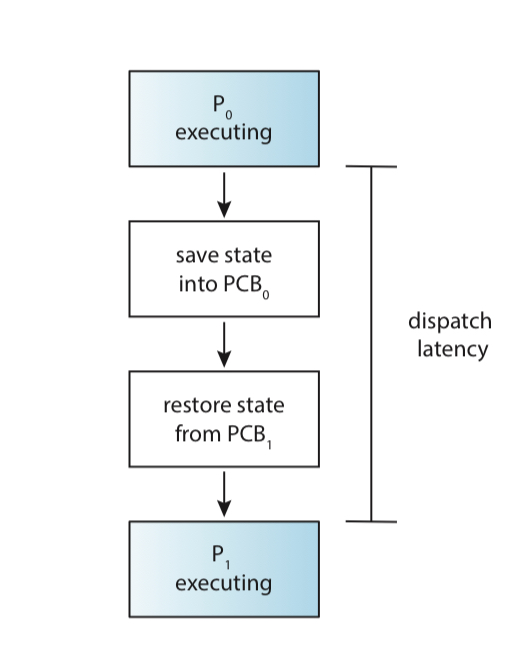
\includegraphics[width=0.4\textwidth]{figures/dispatch-latency.jpg}
            \caption{Dispatch latency: the time it takes for the dispatcher to stop one process and perform a context switch to another}
            \label{fig:dispatch-latency}
        \end{figure}
\end{itemize}

\section*{OS Concepts 5.2: CPU Scheduling Criteria}
\addcontentsline{toc}{section}{5.2: CPU Scheduling Criteria}

\begin{itemize}
    \item \textbf{How to characterize different scheduling algorithms?} We can characterize the properties of various scheduling algorithms according to various criteria. We may choose to optimize for the average measure, but sometimes we may want to optimize for the absolute minimum or maximum value.
        \begin{itemize}
            \item \textbf{CPU utilization:} We want to keep the CPU as busy as possible. CPU utilization is just the inverse of the percentage the time spent idling doing nothing. We would like to maximize this.
            \item \textbf{Throughput:} The number of processes that are completed per time unit. For long processes, this rate may be one process over several seconds; for short transactions it may be tens of processes per second. We would like to maximize this.
            \item \textbf{Turnaround time:} The interval from the time of submission of a process to the time of completion. Turnaround time is the sum of the periods spent waiting in the ready queue, executing on the CPU, and doing I/O. We would like to minimize this.
            \item \textbf{Waiting time:} The scheduling algorithm does not affect the amount of time during which a process executes or does I/O. \textbf{The scheduling algorithm affects only the amount of time that a process spends waiting in the ready queue}. Waiting time is the sum of the periods spent waiting in the ready queue. We would like to minimize this.
            \item \textbf{Response time:} In an interactive system, turnaround time may not be the best criterion (in such a system we don't really care about how long it takes for something to complete fully, we care more about how long it takes to initiate something and then \textit{get a response back}; the process can continue while it's outputting more responses to the user). This measure is the time it takes to first start responding, not the time it takes to output the response. We would like to minimize this.
        \end{itemize}
\end{itemize}

\section*{OS Concepts 5.3: CPU Scheduling Algorithms}
\addcontentsline{toc}{section}{5.3: CPU Scheduling Algorithms}

\subsection*{5.3.1: First Come First Served (FCFS) Scheduling}
\addcontentsline{toc}{subsection}{5.3.1: First Come First Served (FCFS) Scheduling}

\begin{itemize}
    \item \textbf{How does FCFS scheduling work?} This is by far the simplest scheduling algorithm. With this algorithm, the process that requests to use the CPU is allocated the CPU first. This is easily implemented with a FIFO queue. When a process enters the ready queue, its PCB is linked onto the tail of the queue. When the CPU becomes free, the CPU is allocated the process at the head of the queue. This allocated process now running on the CPU is then removed from the queue.
    \item \textbf{FCFS Gantt Chart Visualization?} Figure \ref{fig:fcfs-scheduling}.
        \begin{figure}[ht]
            \centering
            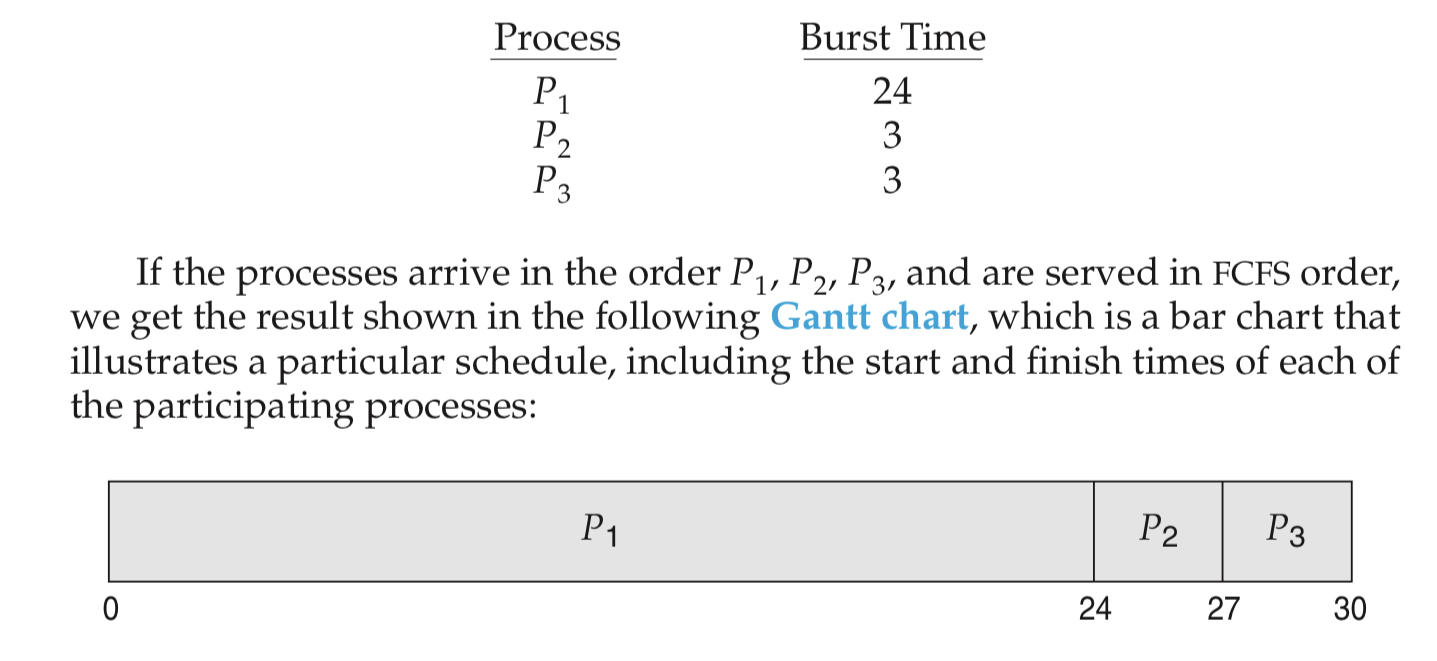
\includegraphics[width=0.7\textwidth]{figures/fcfs-scheduling.jpg}
            \caption{FCFS Scheduling}
            \label{fig:fcfs-scheduling}
        \end{figure}
    \item \textbf{What are some downsides of FCFS scheduling?} The average waiting time can become quite long. In the gantt char visualization (figure \ref{fig:fcfs-scheduling}), the short processes at the end of the queue have to wait for a long time because of the one long process at the beginning of the queue.
    \item \textbf{Is FCFS preemptive or cooperative?} FCFS is cooperative, as once the CPU has been allocated to a process, that process keeps the CPU until it released the CPU, either by terminating (process transitions to terminated state) or by requesting I/O (process transitions to waiting state).
\end{itemize}

\subsection*{5.3.2: Shortest Job First (SJF) Scheduling}
\addcontentsline{toc}{subsection}{5.3.2: Shortest Job First (SJF) Scheduling}

\begin{itemize}
    \item \textbf{How does SJF scheduling work?} The SJF algorithm simply assigns the CPU the process with the smallest upcoming CPU burst. If the upcoming CPU bursts of two processes are the same, FCFS scheduling is used to break the tie. Note that SJF cares about the upcoming \textit{CPU burst}, rather than its total length (since once a CPU burst is over the process does I/O and transitions to the waiting state anyways, not possible to schedule such a process). Algorithm is provably optimal in that it minimizes the average waiting time for a given set of processes (moving a short process before a long one decreases the waiting time of the short process more than it increases the waiting time of the long process). SJF is a special case of the general priority-scheduling algorithm.
    \item \textbf{How is the length of the CPU burst known for SJF scheduling?} There is no way to know the length of the next CPU burst (we can't look into the future!). However, we can use historical data to approximate this. The next CPU burst is generally prediceted as an exponential average (basically weighted sum of previous actual CPU burst length and previous CPUR burst length prediction) of the measured lengths of previous CPU bursts (look into textbook p.208 for full details).
    \item \textbf{SJF Gantt Chart Visualization?} Figure \ref{fig:sjf-scheduling}. All processes have arrived at the same time in this scenario.
        \begin{figure}[ht]
            \centering
            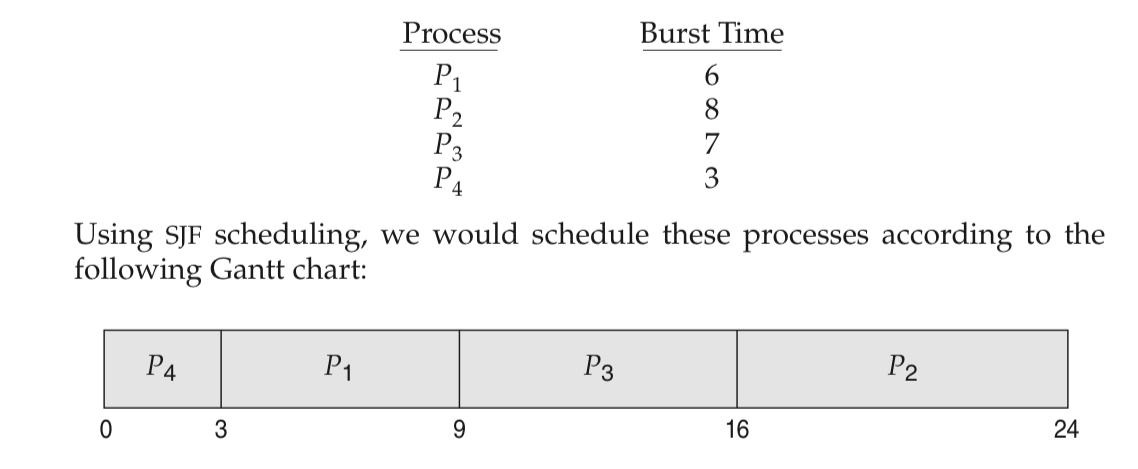
\includegraphics[width=0.7\textwidth]{figures/sjf-scheduling.jpg}
            \caption{SJF Scheduling}
            \label{fig:sjf-scheduling}
        \end{figure}
    \item \textbf{Is SJF preemptive or cooperative?} SJF can be either preemptive or cooperative. The choice arises when a new process arrives at the ready queue while a previous process is still executing. The upcoming (predicted) CPU burst of the newly arrived process may be shorter than what is \textit{left} of the currently executing process. In this situation:
        \begin{itemize}
            \item A \textbf{preemptive} SJF algorithm will preempt the currently executing process
            \item A \textbf{cooperative} SJF algorithm will allow the currently running process to finish its CPU burst, and the schedule the newly arrived process. This is sometimes called shortest remaining time first scheduling.
        \end{itemize}
    \item \textbf{Preemptive SJF Gantt Chart Visualization?} Figure \ref{fig:sjf-preemptive-scheduling}.
        \begin{figure}[ht]
            \centering
            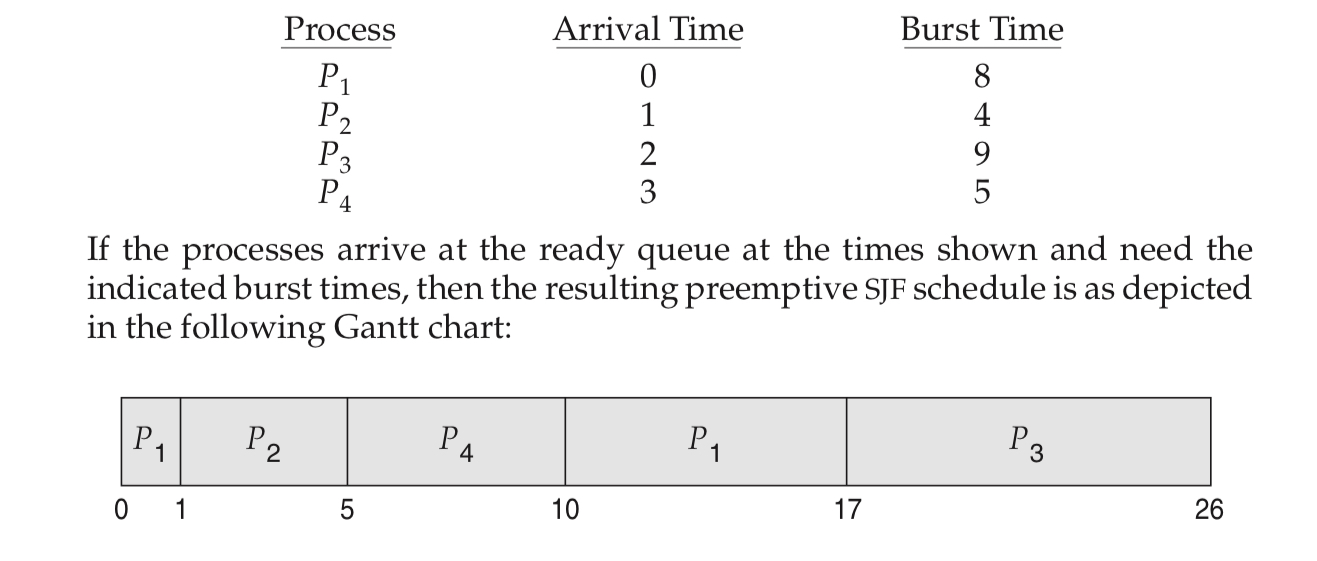
\includegraphics[width=0.7\textwidth]{figures/sjf-preemptive-scheduling.jpg}
            \caption{Preemptive SJF Scheduling. Notice how process \(P_1\) is preempted.}
            \label{fig:sjf-preemptive-scheduling}
        \end{figure}
\end{itemize}

\subsection*{5.3.3: Round Robin (RR) Scheduling}
\addcontentsline{toc}{subsection}{5.3.3: Round Robin (RR) Scheduling}

\begin{itemize}
    \item \textbf{How does RR scheduling work?} RR scheduling is similar to FCFS, but preemption is added to enable the system to switch between processes. A small unit of time, called a \textbf{time slice} (or time quantum), is defined (typically 10 to 100 milliseconds on modern OS's). The ready queue is treated as a circular queue (ring buffer). The CPU scheduler goes around the ready queue, allocating the CPU to each process for a time interval for up to 1 time slice. The scheduler picks the first process from the ready queue, sets a timer to interrupt after 1 time slice, and dispatches the process. One of two things may now happen:
        \begin{itemize}
            \item The process may have a CPU burst of \textbf{less} than 1 time slice. In this case, the process itself will release the CPU voluntarily. The scheduler will then proceed to the next process in the ready queue.
            \item The process may have a CPU burst of \textbf{more} than 1 time slice. In this case, the timer will go off and will cause an interrupt to the OS. A context switch will be executed, and the the preempted process will be put at the tail of the ready queue. The CPU scheduler will then select the next process in the ready queue.
        \end{itemize}
    \item \textbf{Round Robin Gantt Chart Visualization?} Figure \ref{fig:rr-scheduling}.
        \begin{figure}[ht]
            \centering
            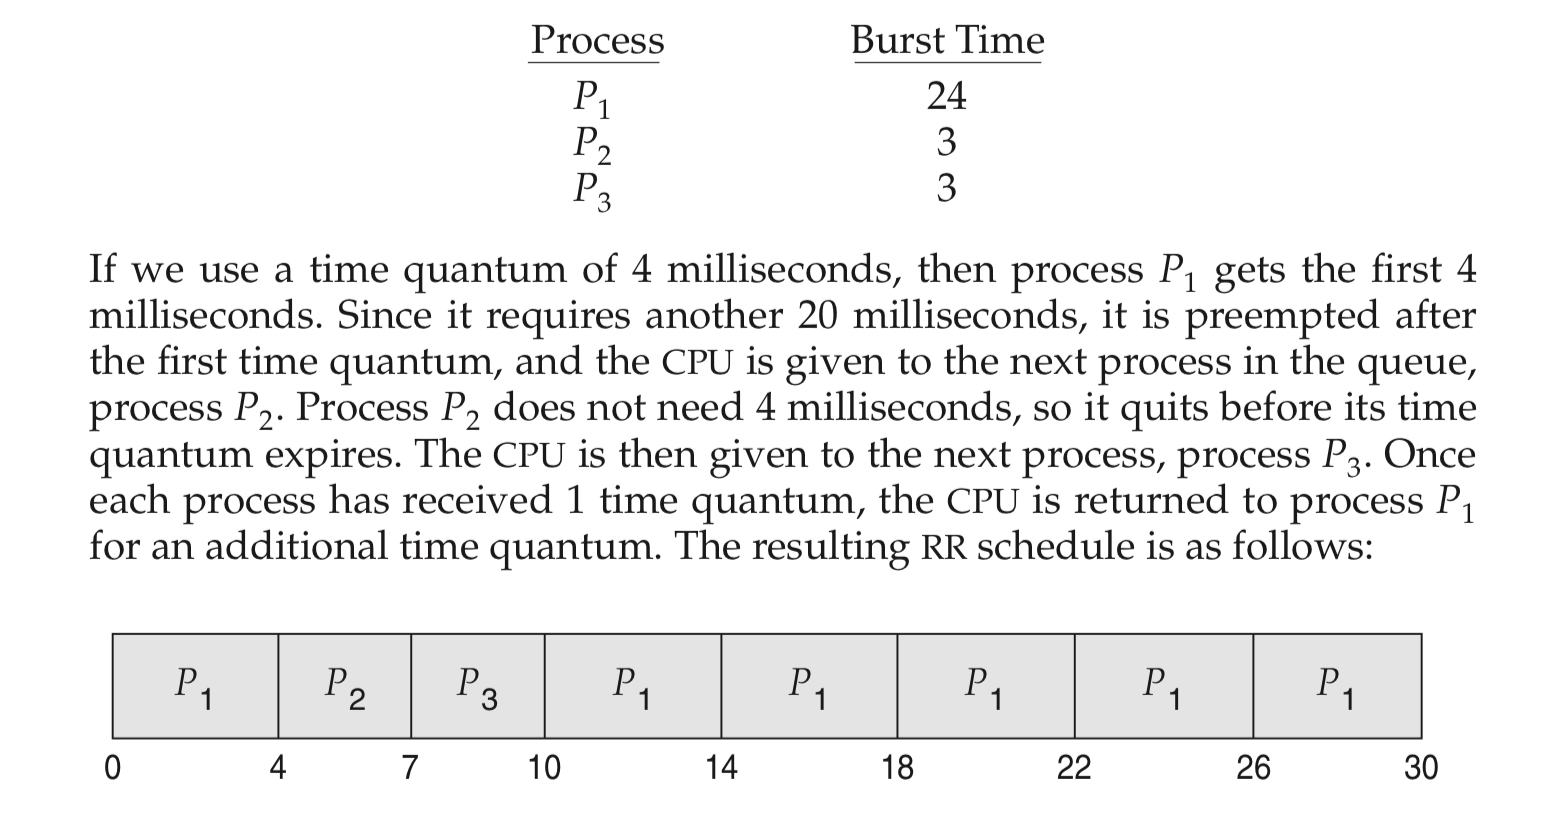
\includegraphics[width=0.7\textwidth]{figures/rr-scheduling.jpg}
            \caption{Round robin scheduling}
            \label{fig:rr-scheduling}
        \end{figure}
    \item \textbf{What are some downsides with RR scheduling?} The average waiting time under the RR algorithm is often long. This is because a process that exceeds its time slice, gets preempted and booted to the back of the ready queue, which means processes that often exceed their time slices have to wait for their turn in the ready queue many times over.
    \item \textbf{How long should the time slice be?} The performance of the RR algorithm depends heavily on the size of the time slice. If the time slice is extremely large, RR is the same as FCFS. In contrast, if the time slice is extremely small, RR can result in a large number of context switches (overhead, leads to wasted time). We want the time slice to be large with respect to the context switch time. If the context switch time is approximately 10 percent of the time slice, then about 10 percent of the CPU time will be spent in context switching (not necessarily true for other algorithms like FCFS, FCFS for example rarely context switches). A rule of thumb is that 80 percent of CPU bursts should be shorter than the time slice.
\end{itemize}

\subsection*{5.3.4: Priority Scheduling}
\addcontentsline{toc}{subsection}{5.3.4: Priority Scheduling}

\begin{itemize}
    \item \textbf{How does priority scheduling work?} Each process is associated with a priority, and the CPU is simply allocated to the process with the highest priority. Eqaul priority processes are scheduled in FCFS order. An SJF algorithm is a special case of priority scheduling: SJF is simply a priority algorithm where the priority is the inverse of the (predicted) upcoming CPU burst. Note that some systems use low numbers to represent low priority, while others use low numbers for high priority (in textbook low number represents high priority).
    \item \textbf{How are process priorities determined?} Process priority can be defined internally by using some measurable quantity or quantities: for example time limits, memory requirements, the number of open files, and the ratio of average I/O burst to average CPU burst. External priorities are set by criteria outside the OS, for example the importance of the process to the OS user, the type and amount of funds begin paid for computer use, and other often political factors.
    \item \textbf{Priority Scheduling Gantt Chart Visualization?} Figure \ref{fig:priority-scheduling}.
        \begin{figure}[ht]
            \centering
            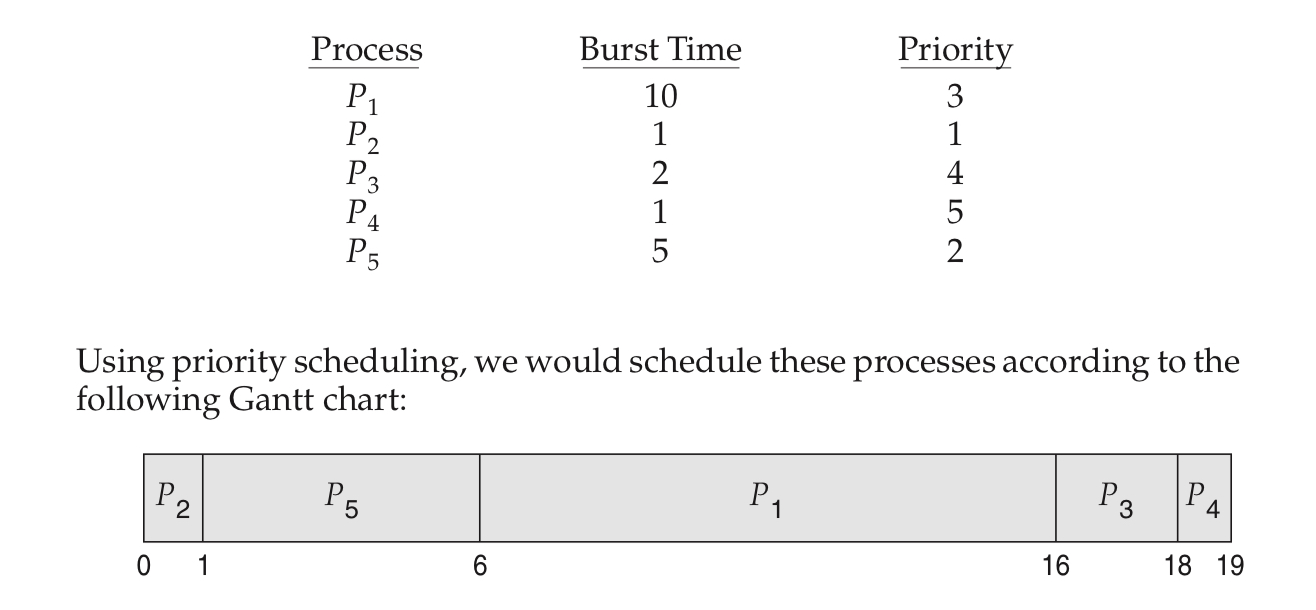
\includegraphics[width=0.7\textwidth]{figures/priority-scheduling.png}
            \caption{Priority scheduling}
            \label{fig:priority-scheduling}
        \end{figure}
    \item \textbf{Is priority scheduling preemptive or cooperative?} Priority scheduling can be either preemptive or cooperative. The choice arises when a new process arrives at the ready queue while a previous process is still executing:
        \begin{itemize}
            \item A \textbf{preemptive} priority scheduling algorithm will preempt the CPU if the priority of the newly arrived process is higher than the priority of the currently running process.
            \item A \textbf{cooperative} priority scheduling algorithm will simply put the new process at the head of the ready queue.
        \end{itemize}
    \item \textbf{What is a major issue with priority scheduling?} A major issue with priority scheduling is indefinitely blocking, or \textbf{starvation}. It's possible that low priority processes never get selected to be run on the CPU, since there are always higher priority processes to run first. It is possible that the profess will eventually be run when there are hardly any other processes keeping the computer busy (e.g. 2AM Sunday when system is lightly loaded), or the system may crash eventually and these unfinished low priority processes are just lost (I assume the high priority processes are also lost then?).
    \item \textbf{How can the issue of starvation be solved?} One solution is to use \textbf{aging}: aging gradually increases the priority of processes that wait in the system for a long time, so that eventually they will have a priority high enough to actually be selected. Another option is to combine round robine and priority scheduling so that the system executes the highest priority processes, and runs process with the \textbf{same priority} using round robin (basically given equal priority processes, rotate among them using round robin).
\end{itemize}

\subsection*{5.3.5: Multilevel Queue Scheduling}
\addcontentsline{toc}{subsection}{5.3.5: Multilevel Queue Scheduling}

\begin{itemize}
    \item \textbf{How does multilevel queue scheduling work?} Simple scheduling algorithms have just a single ready queue. Sometimes it is practical to have separate queues for distinct priority levels: multilevel queue scheduling simply schedules the process in the highest-priority queue, and can be combined with round robin to rotate equal priority processes among each other. Processes are permanently assigned to a specific queue and \textbf{may not} be moved between queues. In addition, there must be scheduling among the queue themselves:
        \begin{itemize}
            \item One possibility is to use fixed-priority queue preemptive scheduling: each queue has absolute priority over lower-priority queues. No processes in lower-priority queues get to run until all higher priority processes are finished. If a low priority process is running and a higher priority process entered its respective ready queue, the low priority process will be preempted to make way for the higher priority process.
            \item Another option is to time slice among the queues: each queue gets a certain portion of CPU time, during which it can then schedule its various processes (e.g. high-priority queue can be given 80 percent of CPU time and 20 percent for low-priority queue).
        \end{itemize}
    \item \textbf{How can multilevel queue scheduling be useful?} A useful application of multilevel queue scheduling is categorizing processes based on process type: for example real-time processes, system processes, interactive processes, and batch processes.
\end{itemize}

\subsection*{5.3.6: Multilevel Feedback Queue Scheduling}
\addcontentsline{toc}{subsection}{5.3.6: Multilevel Feedback Queue Scheduling}

\begin{itemize}
    \item \textbf{How does multilevel feedback queue scheduling work?} Multilevel feedback queue scheduling is basically multilevel queue scheduling but processes are allowed to move between different queues of different priority. The main concept is to move processes among different queues according to their CPU bursts: if a process uses too much CPU time, it will be moved to a lower-priority queue, and a process that waits too long in a lower-priority queue may be moved to a higher-priority queue. This leaves I/O bound and interactive processes (characterized by short CPU bursts) in the higher-priority queues. Moving queues to higher-priority queues also helps prevent starvation. This makes a multilevel feedback queue scheduler the most general scheduling algorithm (can be fine-tuned for system), but also makes it the most complex to implement.
\end{itemize}

\section*{OS Concepts 5.4: Thread Scheduling}
\addcontentsline{toc}{section}{5.4: Thread Scheduling}

\begin{itemize}
    \item \textbf{Contention Scope:} Contention scope is basically the ``scope'' in which \textit{threads} (not processes) compete for CPU. Scope distinction is important when discussing M:1/M:N vs 1:1 threading models.
        \begin{itemize}
            \item \textbf{Process Contention Scope (PCS):} PCS is when competition for the CPU occurs among threads belonging to the \textit{same process} (thread scheduling mechanism using user-level thread library local to the process - not visible to kernel). This is what happens in M:1 and M:N threading models.
            \item \textbf{System Contention Scope (SCS):} SCS is when competition for the CPU occurs among \textit{all (kernel) threads in the system} (threads scheduled by kernel). Systems using the 1:1 model schedule threads using SCS.
        \end{itemize}
\end{itemize}

\section*{OS Concepts 5.5: Multi-Processor Scheduling}
\addcontentsline{toc}{section}{5.5: Multi-Processor Scheduling}

\subsection*{5.5.1: Approaches to Multi-Processor Scheduling}
\addcontentsline{toc}{subsection}{5.5.1: Approaches to Multi-Processor Scheduling}

\begin{itemize}
    \item \textbf{CPU scheduling in a multiprocessor system:} If multiple CPUs are available, \textbf{load sharing}, where multiple threads may run in \textit{parallel}, becomes possible. Scheduling issues, however, naturally become more complex.
    \item \textbf{Asymmetric Multiprocessing:} One approach to CPU scheduling in a multiprocessor system is to have all scheduling decisions, I/O processing, and other system activities handled by a single processor - the master server. The other processes execute only user code. Exactly what work the master processor and other processors perform differs from system to system.
    \item \textbf{Asymmetric multiprocessing benefits?} Simple to support in the OS because only one core has access to system data structures, reducing the need for data sharing.
    \item \textbf{Asymmetric multiprocessing drawbacks?} The master server becomes a potential bottleneck that reduces overall system performance.
    \item \textbf{Symmetric Multiprocessing (SMP):} Instead of having \textit{asymmetric} responsibilities, in an SMP system all processors are treated the same by the OS, reserving none for special purposes. Used by most multiprocessor systems today.
    \item \textbf{How are threads scheduled to run on which processors on an SMP system?} Two possible strategies:
        \begin{enumerate}
            \item All eligible threads may be in a common ready queue. The downside is that there could be a possible race condition on the shared ready queue (processors may schedule the same thread or threads can get lost from the queue). Locking could be used to protect from this race condition, but would likely be a performance bottleneck as all queue access would require lock ownership.
            \item Each processor may have its own private queue of threads. Does not suffer from locking issues with a shared run queue. The most common approach on SMP systems. May lead to more efficient use of cache memory (processor affinity), but workloads of varying sizes present an issue (addressed by load balancing).
        \end{enumerate}
        Shown in figure \ref{fig:smp-scheduling}.
        \begin{figure}[ht]
            \centering
            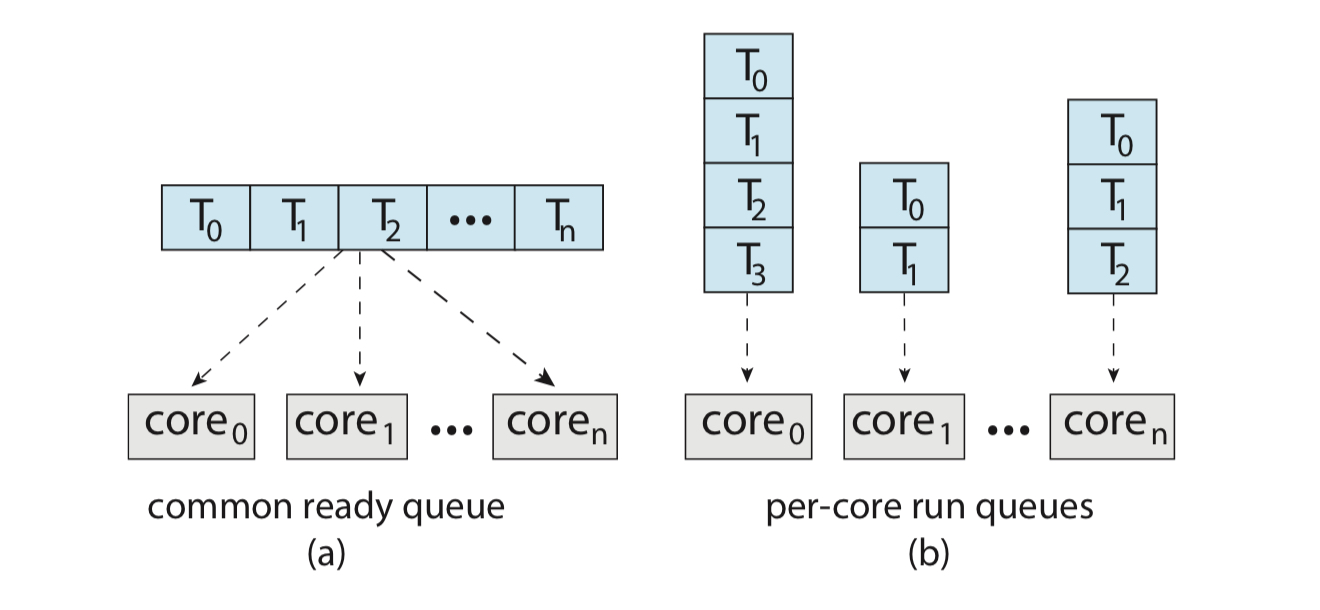
\includegraphics[width=0.7\textwidth]{figures/smp-scheduling.jpg}
            \caption{SMP Scheduling Strategies}
            \label{fig:smp-scheduling}
        \end{figure}
\end{itemize}

\subsection*{5.5.2: Multicore Processors}
\addcontentsline{toc}{subsection}{5.5.2: Multicore Processors}

\begin{itemize}
    \item \textbf{Hardware Threads:} Modern CPUs spend lots of time idle waiting for memory accesses, called \textbf{memory stalls} (because of a cache miss, branch misprediction and consequent pipeline flush, or a data dependency). Some CPUs try to remedy this by using hardware designs in which two (or more) hardware threads are assigned to each core (Intel does this with their hyperthreading technology). This way, when one hardware thread stalls while waiting for memory, the core can switch to another thread. Hardware threads appear as logical CPUs to the OS. Note that the main execution resources (pipeline and execution unit) and caches are shared and only architectural state (e.g. processor registers) is duplicated, which means that the processing core can only execute one hardware thread at a time.
\end{itemize}

\subsection*{5.5.3: Load Balancing}
\addcontentsline{toc}{subsection}{5.5.3: Load Balancing}

\begin{itemize}
    \item \textbf{Why do we need workload load balancing?} In SMP systems, to fully utilize the benefits of having more than one processor we need to make sure the workload among them is balanced: this is called \textbf{load balancing}. Otherwise, one or processors may sit idle while other processors have high workloads.
    \item \textbf{Why is load balancing only necessary on SMP systems with private ready queues?} Load balancing is typically only necessary on SMP systems with per-processor private ready queues: processors on systems with a common ready queue simply take threads from this shared queue, there is no need for load balancing.
    \item \textbf{What are the two main approaches to load balancing?}
        \begin{enumerate}
            \item \textbf{Push Migration:} The OS checks the load on each processor periodically. If there's an imbalance, some threads are \textit{pushed} from overloaded to idle/less-busy processors.
            \item \textbf{Pull Migration:} Occurs when an idle processor pulls a waiting task from a busy processor. Basically like work stealing I guess.
        \end{enumerate}
        These two strategies are not mutually exclusive and are often implemented together on load-balancing systems.
\end{itemize}

\subsection*{5.5.4: Processor Affinity}
\addcontentsline{toc}{subsection}{5.5.4: Processor Affinity}

\begin{itemize}
    \item \textbf{What is processor affinity?} We would like to keep our caches ``warm'' and avoid moving threads to other processors which would cause cache invalidation for the original processor and repopulation of the cache for the new processor. Trying to keep a thread running on the same processor and taking advantage of a warm cache is known as \textbf{processor affinity} (a process has an affinity for the processor on which it is currently running). There is a natural tension between processor affinity and load balancing, as they try to accomplish conflicting tasks.
    \item \textbf{Soft vs Hard Affinity?} Soft affinity is best effort- the OS will try to keep processes running on the same processors, but does not guarantee that it does so (during load balancing). Hard affinity ensures that a processor always gets scheduled on the same processor.
\end{itemize}

\subsection*{5.5.5: Heterogeneous Multiprocessing}
\addcontentsline{toc}{subsection}{5.5.5: Heterogeneous Multiprocessing}

\begin{itemize}
    \item \textbf{What is heterogeneous CPU multiprocessing (HMP)?} Commonly found on mobile systems, some multicore architectures feature designs that use cores that run the same instruction set, yet vary in terms of their clock speed and power management (can reduce power consumption of a core to the point of even idling it). The intention behind HMP is to better manage power consumption by assigning tasks to certain cores based upon the specific requirements of the task. Known as \textit{big.LITTLE} on ARM processors (Firestorm and Icestorm cores in Apple M1).
\end{itemize}

\section*{OS Concepts 5.7: Operating-System Examples}
\addcontentsline{toc}{section}{5.7: Operating-System Examples}

\subsection*{5.7.1: Linux Scheduling}
\addcontentsline{toc}{subsection}{5.7.1: Linux Scheduling}

\begin{itemize}
    \item \textbf{What scheduler is used in Linux?} Introduced in release 2.6.23 (2007!) of the kernel, the \textbf{Completely Fair Scheduler (CFS)} became the default Linux scheduling algorithm.
    \item \textbf{How does the CFS differ from classic scheduling?} The CFS differs from classic preemptive scheduling by not using fixed timeslices and explicitly set priorites. The CFS also implements real-time scheduling using the POSIX standard.
    \item \textbf{How does CFS schedule tasks?} The CFS scheduler has a \textit{targeted latency}, which is an interval of time in which every task should run at least once. Ideally we would like the targeted latency to be infinitely small, as this would mean that every task is run in any given timespan (e.g. 5ns, 1ms, etc.). In practice, the targeted latency is set to 20ms by default. Each runnable task gets a \(1/N\) slice of the target latency, where \(N\) is the number of tasks (this is where the term fair comes from, giving a fair \(1/N\) to each task). \begin{sloppypar} The \(1/N\) slice is indeed a timeslice, but this value is dynamic depending on the number of tasks in the system (tasks finish and new tasks are created all the time). Additionally, this slice is weighted by the \textbf{nice value} of the task: ranging from -20 to 19, lower nice values mean that the \(1/N\) will actually be correspondingly greater, and vice versa. \end{sloppypar} \begin{sloppypar} The CFS tracks how long each task has run by maintaining the \textbf{virtual runtime} \texttt{vruntime} variable. The \texttt{vruntime} is what is weighted by the nice value (lower nice values \(\rightarrow\) lower weighted \texttt{vruntime}). The CFS selects the task that has the smallest \texttt{vruntime} value (the task with the lowest runtime is the task that deserves the most to run next). The runqueue is implemented as a red-black tree using \texttt{vruntime} values as keys. \end{sloppypar} 
    \item \textbf{How does CFS implement load balancing?} The CFS supports load balancing, that is also NUMA aware and tries to minimize the migration of threads. Since migrating threads may result in memory access penalties (cache invalidation or accessing non-local memory across the system interconnect on NUMA systems), CFS addresses this using a hierachical system of \textbf{scheduling domains} (figure \ref{fig:cfs-load-balancing}). A scheduling domain is a set of CPU cores that threads can be balanced among. The cores are grouped by how they share the resources of the system (e.g. first domain level are cores that only share L2 cache, next domain level are NUMA nodes that share L3 cache, etc.). The CFS balances loads within these domain levels, beginning at the lowest level of the hierarchy (try to migrate threads in the smallest domain level first, e.g. cores sharing L2 cache, and only reluctanly migrate threads across higher level domains like NUMA nodes).
    \begin{figure}[ht]
        \centering
        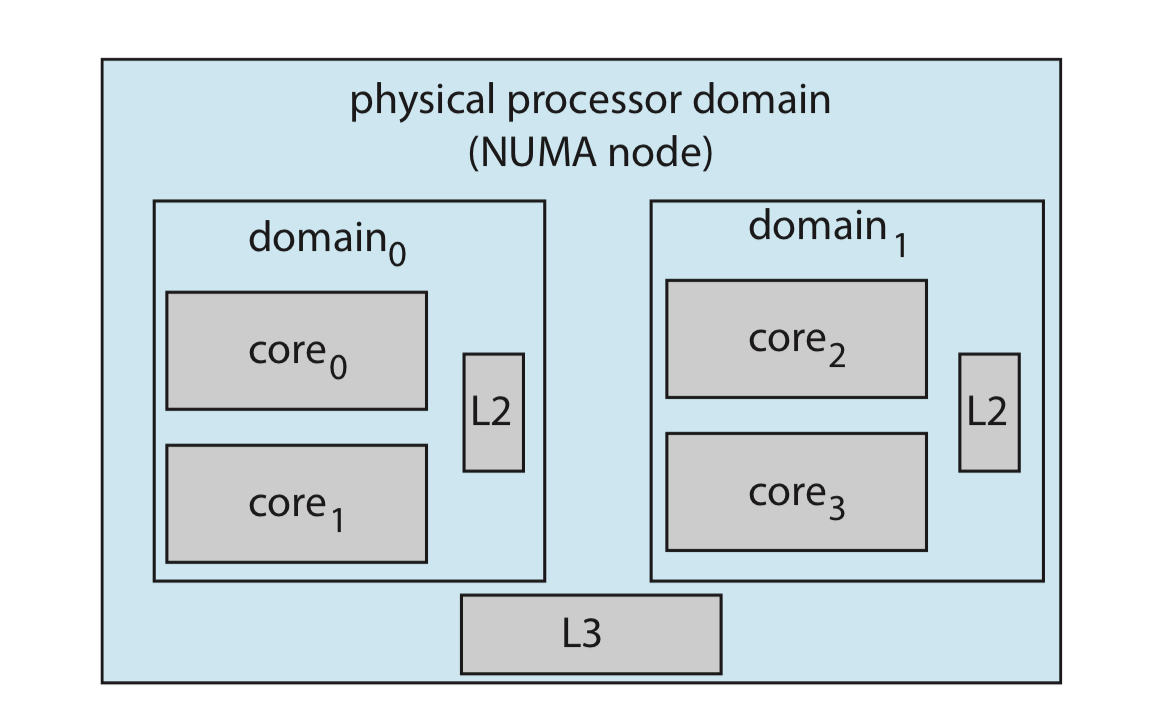
\includegraphics[width=0.6\textwidth]{figures/cfs-load-balancing.jpg}
        \caption{Linux CFS load balancing}
        \label{fig:cfs-load-balancing}
    \end{figure}
\end{itemize}

\section*{OS Concepts 6.1: Synchronization Background}
\addcontentsline{toc}{section}{6.1: Synchronization Background}

\begin{itemize}
    \item \textbf{What is a race condition?} A situation where several threads access and manipulate the same data concurrently and the outcome of the execution depends on the specific order in which the accesses takes place.
    \item \textbf{How do we protect against race conditions?} Threads need to be synchronized in some way to protect against race conditions.
\end{itemize}

\section*{OS Concepts 6.2: The Critical Section Problem}
\addcontentsline{toc}{section}{6.2: The Critical Section Problem}

\begin{itemize}
    \item \textbf{What is a critical section?} A critical section is a segment of code in which a process may be accessing and modifying data that is shared with at least one other process, and thus has to be executed as an atomic action. We want only \textbf{one process} at most to be executing its critical section at a time. A critical section is illustrated in figure \ref{fig:critical-section}. This is especially important in the context of OS's, since many kernel data structures (e.g. open file lists) are accessed by a lot of different kernel-mode processes.
    \begin{figure}[ht]
        \centering
        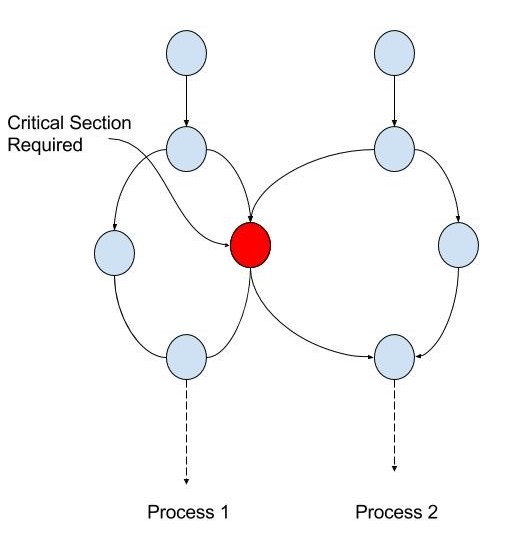
\includegraphics[width=0.45\textwidth]{figures/critical-section.jpg}
        \caption{Two processes with the same critical section}
        \label{fig:critical-section}
    \end{figure}
    \item \textbf{How can the critical-section problem be solved?} A solution to the critical-section must satisfy the following three requirements:
    \begin{enumerate}
        \item \textbf{Mutual Exclusion:} Only one process at a time may be active in the critical-section.
        \item \textbf{Progress:} Processes will cooperatively determine which process will next enter the critical-section.
        \item \textbf{Bounded Waiting:} There must be an upper limit to how long a process will wait before it can enter the critical section.
    \end{enumerate}
\end{itemize}

\section*{OS Concepts 6.3: Peterson's Solution}
\addcontentsline{toc}{section}{6.3: Peterson's Solution}

\begin{itemize}
    \item \textbf{What is Peterson's solution?} Peterson's solution is a software approach to the critical-section problem. It is an algorithm that allows two processes to use shared data without conflict (can be generalized to more than two processes). Since most modern processors and/or compilers reorder memory accesses that have no dependencies, Peterson's solution is not guaranteed to work correctly on these systems.
\end{itemize}

\section*{OS Concepts 6.4: Hardware Support for Synchronization}
\addcontentsline{toc}{section}{6.4: Hardware Support for Synchronization}

\subsection*{6.4.1: Memory Barriers}
\addcontentsline{toc}{subsection}{6.4.1: Memory Barriers}

\begin{itemize}
    \item \textbf{What is memory reordering?} Modern compilers and processors often reorder memory accesses to maximize performance. Compilers can do this reordering at compile time at the machine instruction level, and processors can do this at runtime (out of order execution).
    \item \textbf{What are memory models?} The (hardware) memory model of a system specifies the types of processor memory reordering at runtime that can be expected, relative to given source machine instruction code. Software memory models exist as well, that are supposed to standardize the semantics of memory across arbitrary compilers and platforms.
    \item \textbf{Weak vs strong memory models?} Memory models lie on a spectrum, from weak to strong. Weaker memory models permit more memory reordering (e.g. ARM), while stronger memory models (e.g. x86) are more stringent on what reordering is allowed.
    \item \textbf{How do we protect ourselves from memory reordering on multiprocessor systems?} We can use \textbf{memory barriers} to ensure that all loads/stores are completed before any subsequent loads/stores (basically enforce our desired memory ordering and not allow the compiler/processor to perform any memory reordering). This naturally comes at the performance cost of not doing out-of-order execution.
\end{itemize}

\subsection*{6.4.2: Hardware Instructions}
\addcontentsline{toc}{subsection}{6.4.2: Hardware Instructions}

\begin{itemize}
    \item \textbf{What instructions does HW give us to perform atomic operations?} Many computer systems have special hardware instructions that allow us to perform atomic operations (one uninterruptible unit). These instructions can be used to enforce mutual exclusion.
    \item \textbf{Test-and-set} Test-and-set is an atomic instruction provided by the hardware. It writes 1/true (set) to a memory location and returns its old value as a single atomic operation (where we can test the old value). This can be used to implement mutual exclusion using a lock. Pseudocode of the \textit{effects} of test-and-set are shown in figure \ref{fig:test-and-set} (note that this is just an illustration in pseudocode, this must be implemented as an atomic instruction in hardware).
    \begin{figure}[ht]
        \centering
        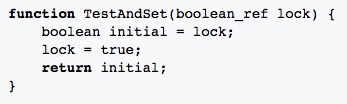
\includegraphics[width=0.45\textwidth]{figures/test-and-set.jpg}
        \caption{Pseudocode of test-and-set}
        \label{fig:test-and-set}
    \end{figure}
\item \textbf{Compare-and-swap} Compare-and-swap (CAS) is an atomic instruction provided by the hardware. It can be used to implement mutual exclusion (using a lock). Basically CAS, in one atomic operation, tests to see if the current value is the same as our old value, and only then updates it with a new value. It always returns the old value. Pseudocode is shown in figure \ref{fig:cas}. On x86 platforms CAS is implemented using the \texttt{lock cmpxchg} instruction.
    \begin{figure}[ht]
        \centering
        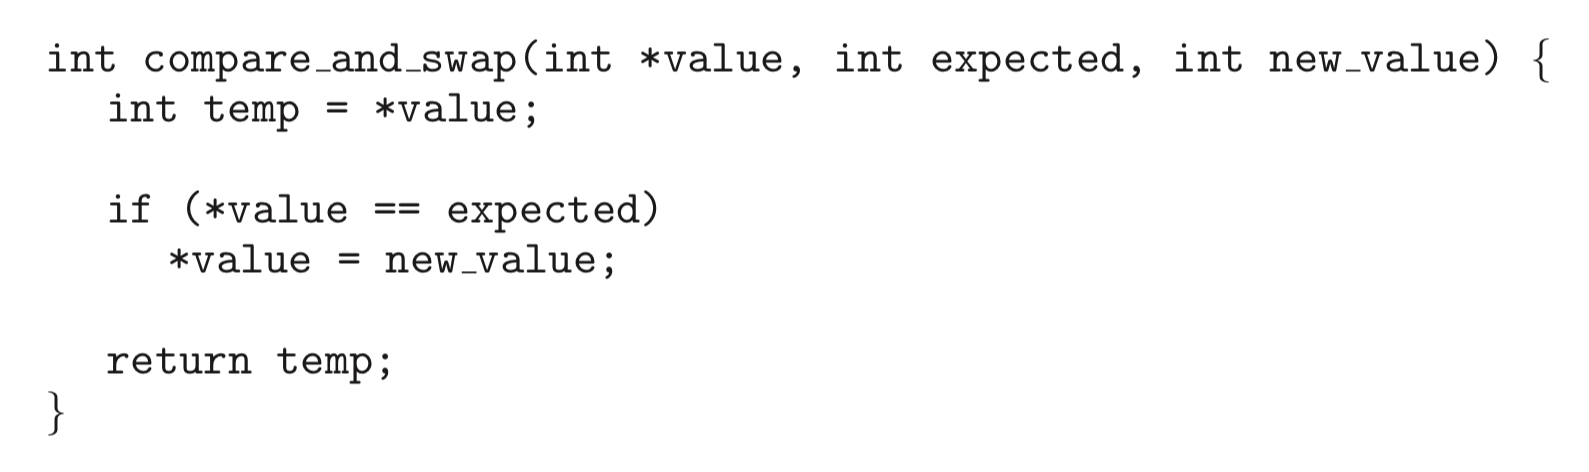
\includegraphics[width=0.7\textwidth]{figures/cas.jpg}
        \caption{Pseudocode of CAS}
        \label{fig:cas}
    \end{figure}
\end{itemize}

\subsection*{6.4.3: Atomic Variables}
\addcontentsline{toc}{subsection}{6.4.3: Atomic Variables}

\begin{itemize}
    \item \textbf{What are atomic variables?} Typically, instructions like test-and-set and CAS are not used directly to provide mutual exclusion. Rather, they are used as basic building blocks for higher level abstractions to solve the critical-section problem. These instructions can be used to implement \textbf{atomic variables}, which provide atomic operations on basic data types like integers and booleans.
\end{itemize}

\section*{OS Concepts 6.5: Mutex Locks}
\addcontentsline{toc}{section}{6.5: Mutex Locks}

\begin{itemize}
    \item \textbf{What are mutex locks?} Mutex locks can be used to protect critical sections and thus prevent race conditions. A process must acquire the lock (mutual exclusion) before entering a critical section, and release the lock when it exits the critical section.
    \item \textbf{Why use mutex locks over hardware instructions like CAS?} Hardware instructions like CAS are complicated and easy to get wrong, so higher level abstractions like mutexes are built upon them instead.
    \item \textbf{What happens if a process attempts to acquire a lock that is already acquired by another process?} This depends on the exact type of mutex implementation, but for something like a spinlock it simply blocks until the lock is release by the other process. With spinlocks, the fact that a process simply ``spins'' and wastes CPU cycles while it waits on the lock to be released is not great for performance, but a spinlock may be preferable if the lock is only held for a short duration (avoid context switch).
\end{itemize}

\section*{OS Concepts 6.6: Semaphores}
\addcontentsline{toc}{section}{6.6: Semaphores}

\begin{itemize}
    \item \textbf{What is synchronization?} In computer science, synchronization means the requirements pertaining to the order of specific events. For example, \textbf{serialization} is when we are concerned with event \(A\) happening before event \(B\) (\(A \prec B\)), and \textbf{mutual exclusion} is when we are concerned with events \(A\) and \(B\) \textit{not} happening at the same time (\(A \prec \succ B\), either \(A\) precedes \(B\) or \(B\) precedes \(A\)).
    \item \textbf{What is a semaphore?} A semaphore is just an integer variable that, apart from initialization, is accessed only through two standard atomic operations: \texttt{wait()} (decrement the integer) and \texttt{signal()} (increment the integer). If a process executes the \texttt{wait()} operation and decrements the integer and it is now negative, the thread blocks (or suspends) itself and cannot continue until the integer is incremented by other processes to be positive again. When a process executes the \texttt{signal()} operation and there are other processes waiting, one of the waiting thread gets unblocked/resumed. Semaphore operations \textbf{must} be executed atomically: this is done using an atomic read-modify-write hardware instruction, usually a test-and-set instruction (or alternatively by simply disabling hardware interrupts on a single-processor environments).
    \item \textbf{What happens when \texttt{wait()} (decrement) is executed and the semaphore is negative?} When a process attempts to \texttt{wait()} (decrement) a semaphore and the integer value is now negative, it can either choose to spin (busy wait) or go to sleep. Spinning can be very wasteful in many situations; the process can instead go to sleep (suspend itself) and it will be added to a queue associated with the semaphore. When another process executes the \texttt{signal()} operation (increment) on the semaphore, the semaphore will choose a process from the queue (we have flexibility with which queue we use; can be FIFO, priority queue, etc.) and wake it up (change the process from the waiting state to the ready state, at which point it may be selected by the CPU scheduler).
    \item \textbf{What does the value of the semaphore integer represent?} If the integer is positive, it represents the number of processes that can decrement without blocking/suspending. If it is negative, it represents the number of processes that are currently blocked/suspended and waiting for the semaphore to be positive again. If it is zero, it means there are no processes blocked/suspending, but if a process does try to decrement, it will be blocked/suspended.
    \item \textbf{What are semaphores used for?} Semaphores can be used for a variety of synchronization problems, but the simplest and easiest use of them is for \textbf{signaling} (serialization of events). Signaling is when one process sends a signal to another process to indicate that something has occurred. Try not to use semaphores to control access to a pool of shared resources (e.g. access to \(n\) number of bathrooms in a coffee shop, a semaphore would only track \textit{how many} bathrooms are free, not specifically \textit{which} bathrooms are free), rather think of it as a bouncer allowing a certain number of people into a nightclub (one shared resource that can be used simultaneously by a bounded number of users). See the \href{https://greenteapress.com/semaphores/LittleBookOfSemaphores.pdf}{Little Book of Semaphores} for more synchronization patterns involving semaphores (semaphores can also be used for mutual exclusion!).
    \item \textbf{Semaphores vs mutexes?} A binary semaphore (integer value always either 0 or 1) at first glance may seem like a mutex, but the semantics are different: a mutex should be used for exclusive access of a shared resource (metaphor: single key to unlock the only bathroom at a coffee shop), while a binary semaphore should be used for one process to signal to another process that an event has occurred (e.g. process \(A\) waits on a semaphore, that is signaled by process \(B\) when some event occurs). With a mutex, the same process locks and unlocks it, while with a semaphore one process can \texttt{wait()} (loosely analogous to locking a mutex) on a semaphore while another process can \texttt{signal()} (loosely analogous to unlocking a mutex). Useful stackoverflow posts: \href{https://stackoverflow.com/a/86021/7162381}{link 1}, \href{https://stackoverflow.com/a/40238/7162381}{link 2}.
\end{itemize}

\section*{OS Concepts 6.7: Monitors}
\addcontentsline{toc}{section}{6.7: Monitors}

\begin{itemize}
    \item \textbf{TODO}
\end{itemize}

\section*{OS Concepts 6.8: Liveness}
\addcontentsline{toc}{section}{6.8: Liveness}

\begin{itemize}
    \item \textbf{What is a deadlock?} A set of processes is in a deadlocked state when \textit{every} process in the set is waiting for an event that can \textit{only} be triggered by another process in the set (that is also waiting on another such event). Basically, every process is waiting for an event to happen that can only be triggered by another process, that is also waiting (for another event). "When two trains approach each other at a crossing, both shall come to a full stop and neither shall start up again until the other has gone."
    \item \textbf{What is priority inversion?} Priority inversion is where a low priority process causes the execution of a higher priority process to be delayed. This can happen when the lower priority process accesses a resource that the high priority process needs to also access, meaning the higher priority process must wait for the lower priority process to first finish with the resource. Even though the high priority process should run since it has a higher priority, it must instead wait on the lower priority process.
    \item \textbf{What is an example of priority inversion?} Suppose there are three processes - \(L, M, \text{and} \; H\) - that have priorities of the order \(L < M < H\). Process \(H\) wants to use a resource currently being accessed by \(L\). Now suppose, process \(M\) becomes runnable, and prempts process \(L\). Indirectly, a process with a lower priority - process \(M\) - has delayed the execution of a higher priority process - process \(H\).
    \item \textbf{How many priority levels must exist for priority inversion to cause a problem?} Priority inversion only exists in systems with more than two priorities.
    \item \textbf{How can priority inversion be avoided?} There are several solutions to avoid priority inversion. One such solution is by implementing a \textbf{priority-inheritance protocol}: all processes that are accessing resources needed by a higher priority process inherit the higher priority until they are finished with the resource (at which point they revert to their original priorities).
\end{itemize}

\section*{OS Concepts 9.1: Main Memory Background}
\addcontentsline{toc}{section}{9.1: Main Memory Background}

\subsection*{9.1.1: Basic Hardware}
\addcontentsline{toc}{subsection}{9.1.1: Basic Hardware}

\begin{itemize}
    \item \textbf{What kinds of memory can a CPU access?} The CPU can only access its registers and the main memory. The machine instructions a CPU executes can only use memory addresses that refer to main memory (can also of course use register names in instructions). If the desired data is not in memory (e.g. in disk), it must be moved there first before the CPU can operate on it.
    \item \textbf{Why do processes need separate memory spaces?} The processes running on your computer need to somehow share the main memory. Processes should not be able to access the memory of other processes, because this could cause corruption (process A messing around with the memory of process B, we also don't want processes messing around in the kernel) or security vulnerabilities. Consequently, each process is given it's own separate address space.
    \item \textbf{How do we protect processes from accessing each others memory spaces?} Process memory protection must be provided by the hardware, because the OS does not intervene between the CPU and its memory accesses (software intervention would be way too slow). Each process has its own separate memory space: hardware needs the ability to determine the range of legal addresses that the process may access. Hardware can implement this in several different ways.
\end{itemize}

\subsection*{9.1.2: Address Binding}
\addcontentsline{toc}{subsection}{9.1.2: Address Binding}

\begin{itemize}
    \item \textbf{How do programs determine the memory addresses they need to access?} Addresses in the source program are generally symbolic (i.e. variables). Binding these symbolic addresses to actual physical addresses may occur during any of comiple, load, or runtime. Most operating systems bind addresses at runtime - this requires virtual to physical address translation implemented in the hardware.
\end{itemize}

\subsection*{9.1.3: Logical vs. Physical Address Space}
\addcontentsline{toc}{subsection}{9.1.3: Logical vs. Physical Address Space}

\begin{itemize}
    \item \textbf{Logical (Virtual) Address:} An address generated by the CPU. The user program only ever deals with virtual addresses.
    \item \textbf{Physical Address:} The address seen by the memory unit (the address loaded into the memory-address register).
    \item \textbf{Compile/Load time vs Runtime Binding:} Binding addresses at either compile or load time generates identical logical and physical addresses. Runtime address binding, however, results in differing logical and physical addresses (differing because program has no way of knowing where it will be located in physical memory, uses virtual addresses and basically punts the decision to the MMU of what physical memory addresses to use later until runtime).
    \item \textbf{Logical Address Space:} The set of all logical addresses generated by a program.
    \item \textbf{Physical Address Space:} The set of all physical addresses corresponding to the logical addresses of a program.
    \item \textbf{How is the runtime mapping from virtual to physical addresses done?} The runtime mapping is done by a hardware device called the memory management unit (MMU). There are multiple methods to implement such a mapping (e.g. variable partition allocation and paging).
\end{itemize}

\subsection*{9.1.4: Dynamic Loading}
\addcontentsline{toc}{subsection}{9.1.4: Dynamic Loading}

\begin{itemize}
    \item \textbf{What is dynamic loading?} Dynamic \textbf{loading}, not linking! Typically, the entire program and its data needs to be in physical memory for the process to execute. With dynamic loading, a routine is not loaded into memory until it is actually called. All routines are kept on disk in a relocatable load format. Useful for when large amounts of code are needed to handle infrequent cases, keeps memory usage lower. Does not require special support from the OS.
\end{itemize}

\subsection*{9.1.5: Dynamic Linking and Shared Libraries}
\addcontentsline{toc}{subsection}{9.1.5: Dynamic Linking and Shared Libraries}

\begin{itemize}
    \item \textbf{What are dynamically linked libraries (DLLs)?} Also known as shared libraries. Shared libraries are libraries that are linked to user program when the programs are run (linking at runtime). This is usually used with system libraries (e.g. C standard library), since without shared libraries each program would need to include a copy of its language library in the binary (static linking). This would not only increase binary size but also waste main memory when the program is loaded into memory (multiple copies of same library taking up space in memory). Shared libraries can be shared among multiple processes. Dynamic linking also allows libraries to be updated (essentially replaced) without having to relink programs (programs will automatically use this new version at runtime). Generally requires special support from the OS.
    \item \textbf{What is static linking?} With static linking, libraries are treated like any other object file and are combined by the linker into the final binary. Thus, each binary contains its own copy of a library (not the entire library, only the parts the program directly or indirectly uses). This is faster and more portable than dynamic linking, since it does not require the presence of the library on the system where it is run (built into binary).
\end{itemize}

\section*{OS Concepts 9.2: Contiguous Memory Allocation}
\addcontentsline{toc}{section}{9.2: Contiguous Memory Allocation}

\begin{itemize}
    \item \textbf{How do we allocate physical main memory to processes?} The OS must somehow choose what physical memory to allocate to running processes. We would like allocation to be as efficient as possible, both in terms of time to allocate memory and also minimizing memory wasted.
    \item \textbf{What is Variable Partition allocation?} Basically divide physical memory in variable sized paritions to allocate processes to (figure \ref{fig:variable-partitioning}). Each parition contains exactly one process (this also means that the \textbf{entire program} must be loaded into memory, in the partition). This also means that each physical partition is \textbf{contiguous}. The OS keeps a table indicating which parts of memory are available and which are occupied.
    \item \textbf{How does Variable Partitioning allocate and free memory for processes?} The space in memory not occupied by paritions are referred to as \textbf{holes}. When a process arrives and needs memory, the OS searches for a hole that is large enough for this process. We can use either first fit (first hole that is big enough), best fit (smallest hole that is big enough, need to search through all holes), or worse fit (largest hole available, also need to search through all holes). If the hole is too large, it is split into two parts. One part is allocated to the arriving process; the other is returned to the set of holes. When a process terminates, it releases its block of memory, which is then placed back in the set of holes. If the new hole is adjacent to other holes, these adjacent holes are merged to form one larger hole.
        \begin{figure}[ht]
            \centering
            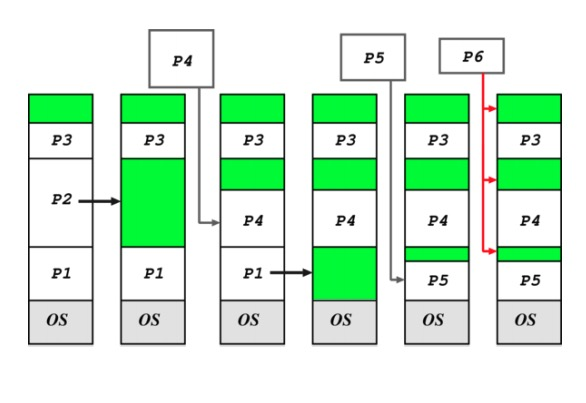
\includegraphics[width=0.5\textwidth]{figures/variable-partitioning.jpg}
            \caption{Variable Partitioning}
            \label{fig:variable-partitioning}
        \end{figure}
    \item \textbf{What is external fragmentation?} Variable partitioning algorithms suffer from external fragmentation: when processes are loaded the free memory space is broken into little pieces. External fragmentation exists when enough total free memory is available, but it is effectively unusable because it is divided into pieces that are too small individually (last column in figure \ref{fig:variable-partitioning}).
    \item \textbf{What is internal fragmentation?} More memory may sometimes be allocated to a process than is requested (e.g. if holes have fixed sizes). This wasted memory is called internal fragmentation.
    \item \textbf{How can we possibly solve external fragmentation?} We can possibly solve external fragmentation using \textbf{compaction}. Basically shuffle memory contents so as to place all free memory together in one block. Compaction is not always possible however: only possible if program relocation is dynamic and done at execution time.
\end{itemize}

\section*{OS Concepts 9.3: Paging}
\addcontentsline{toc}{section}{9.3: Paging}

\begin{itemize}
    \item \textbf{What is paging?} Paging is a memory management scheme that allows a process's physical address space to be non-contiguous. It separates the logical address space from the physical memory space. This concept has many implications: external fragmentation is completely avoided (although internal fragmentation still exists), adds memory protection capabilities, greatly increases the logical address space of processes, and more. 
    \item \textbf{What parts of a computer system are used to implement paging?} Paging requires the support of both the OS and hardware.
\end{itemize}

\subsection*{9.3.1: Basic Paging Concepts/Implementation}
\addcontentsline{toc}{subsection}{9.3.1: Basic Paging Concepts/Implementation}

\begin{itemize}
    \item \textbf{How is physical memory divided?} Physical memory is broken into fixed-sized blocks called \textbf{frames}.
    \item \textbf{How is logical memory divided?} Physical memory is broken into fixed-sized blocks called \textbf{pages}, that are of the same size as physical memory frames.
    \item \textbf{What is a logical memory address composed of?} A logical memory address is divided into two parts: a \textbf{page number} (p) and a \textbf{page offset} (d). The page number is used to index into the page table to look up the physical memory frame, and the offset is the offset of the physical address from the base address of the frame. Shown in figure \ref{fig:logical-address}.
        \begin{figure}[ht]
            \centering
            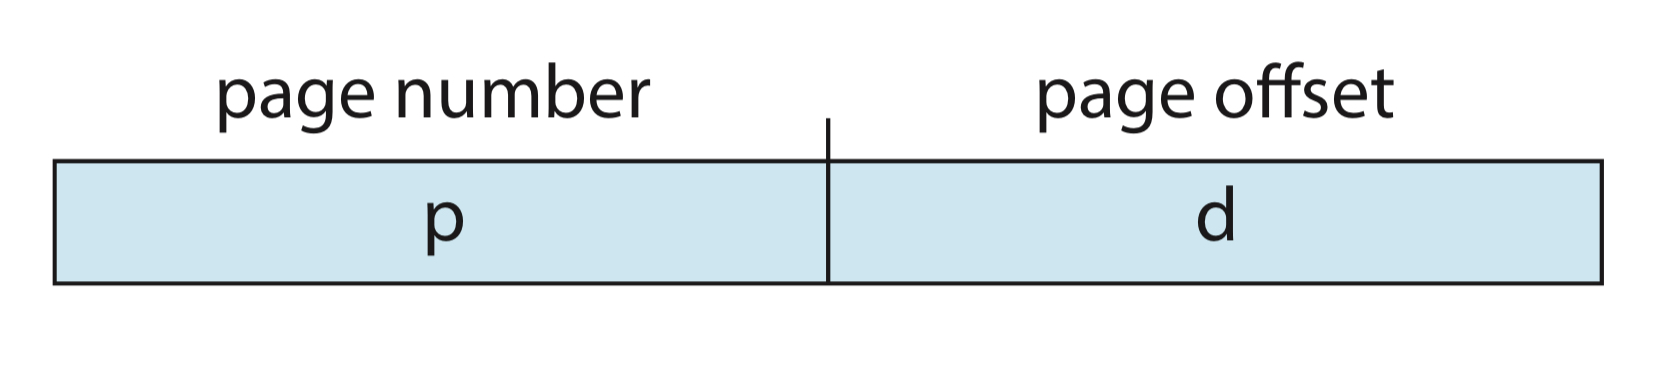
\includegraphics[width=0.5\textwidth]{figures/logical-address.jpg}
            \caption{Structure of a logical address}
            \label{fig:logical-address}
        \end{figure}
    \item \textbf{What is the page table?} The page table is a \textit{per-process} data structure that contains the mappings of page numbers to the base address of the corresponding physical memory frame.
    \item \textbf{How is a logical address translated into a physical address?} The MMU performs the following steps to translate a logical address into a physical address:
        \begin{enumerate}
            \item Extract the page number \(p\) from the logical address.
            \item Use the page number as an index into the process page table, to look up the corresponding physical memory frame number \(f\).
            \item Replace the page number \(p\) in the logical address with the frame number \(f\).
        \end{enumerate}
        The offset \(d\) \textbf{does not change}. The physical address is now comprised of the physical memory frame base address and offset. Process shown in figure \ref{fig:address-translation}.
        \begin{figure}[ht]
            \centering
            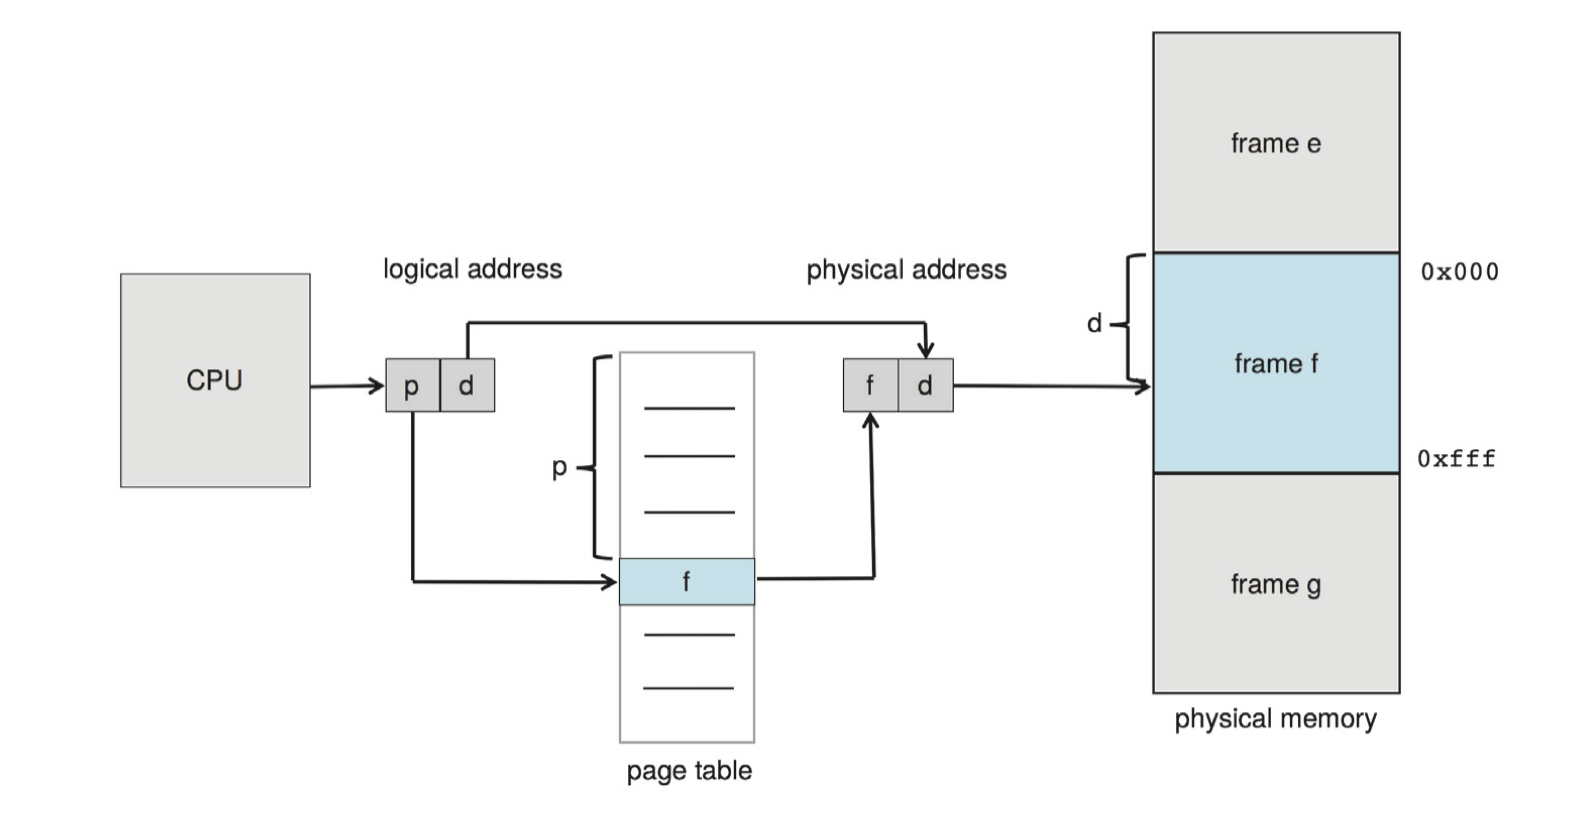
\includegraphics[width=0.8\textwidth]{figures/address-translation.jpg}
            \caption{Illustration of how address translation works}
            \label{fig:address-translation}
        \end{figure}
    \item \textbf{What component decides the page and frame size?} The \textit{hardware} defines both the page and frame sizes.
    \item \textbf{Why are page sizes typically a power of 2?} Page sizes are typically powers of 2 since this means that simply the first \(n\) higher-order bits can be used as the page number. If the page size was not a power of 2, the logical address could not be cleanly separated into a page number and offset (imagine a page size of 9 bytes, the offset would need to be 4 bits long, even though 4 bits can be used to specify up to 16 offsets, this robs a bit that could have been used instead for the page number).
    \item \textbf{Why is there no external fragmentation when using a paging scheme?} There is no external fragmentation because paging does not require contiguous physical memory. Even if the available physical memory frames are fragmented across the memory space, a paging scheme simply picks the fragmented frames and allocates them all to a process. The logical address space from the perspective of a process is still that of a contiguous single dimensional array.
    \item \textbf{Why does internal fragmentation occur when using a paging scheme?} Internal fragmentation still occurs when using a paging scheme, since a process probably requires \(n\) bytes of memory that is not an exact multiple of the page size. An entire page still has to be allocated to cover the ``remainder'' bytes. The worst case is where a process requires \(n\) pages plus \(1\) byte: it would be allocated \(n + 1\) frames.
    \item \textbf{What are the tradeoffs involved in choosing page size?} If process size is independent of page size (uniform distribution of ``remainder'' bytes), we can expect internal fragmentation to average one-half page per process. This suggests that smaller page sizes are desirable. Smaller page sizes, however, means that the page table has to be larger.
    \item \textbf{What is the typical size of a page?} Page sizes have historically grown larger as processes, the data they work with, and main memory have grown larger. Today, page sizes are typically 4KB or 8KB (Linux default is 4KB).
    \item \textbf{What is the programmers/programs view of the address space?} The programmer views the logical address space: a single contiguous array of bytes. The mapping of logical addresses to physical addresses is hidden from the programmer and controlled by the OS.
\end{itemize}

\subsection*{9.3.2: Hardware Support for Paging}
\addcontentsline{toc}{subsection}{9.3.2: Hardware Support for Paging}

\begin{itemize}
    \item \textbf{How is the page table implemented?} The page table for each process is kept in main memory. A \textbf{page-table base register} in hardware contains the address of the page table. Changing page tables in a context switch requires changing only this one register.
    \item \textbf{What is the TLB?} Accessing memory to first index into the page table, and then accessing memory again with the actual physical address is very slow, because of the two accesses to main memory. To solve this, a small and fast hardware cache called the translation look-aside buffer (TLB) is used to cache address mappings (page table entries).
    \item \textbf{What is the typical size of a TLB?} To be able to execute a TLB lookup within a single processor pipeline step (to add no performance penalty), the TLB must be kept small. It is typically between 32 and 1,024 entries in size. Some CPUs implement separate instruction and data TLBs, doubling the number of TLB entries available. Modern processors even have multiple levels of TLBs.
    \item \textbf{What happens when a context switch occurs (TLB entries become invalid)?} When a context switch occurs and the mappings of a new process page table is used, the mappings in the TLB become invalid. One solution is to just flush these entries, and have the cache repopulate itself as memory accesses are made. A more effective strategy is to mark to which process a TLB entry belongs: an \textbf{address-space identifier} (ASID) is used to uniquely identify each process, an only TLB entries with an ASID matching the current process are considered valid. This means mappings for multiple processes can be kept in the TLB simultaneously, reducing the frequency with which mappings need to be repopulated in the cache.
    \item \textbf{What is the typical hit ratio of a TLB?} TLBs typically have hit ratios of 99 percent.
\end{itemize}

\subsection*{9.3.3: Memory Protection using Paging}
\addcontentsline{toc}{subsection}{9.3.3: Memory Protection using Paging}

\begin{itemize}
    \item \textbf{How is memory protection achieved in a paged environment?} Memory protection in a paged environment can easily be accomplished by adding permission bits to page table entries. Example permission bits are read, write, execute, and supervisor (process must be in kernel mode). These permission bits can be checked everytime when address translation is performed. If an instruction violates these permissions, the processor triggers a fault that transfers control to an exception handler in the kernel (typically reported as a ``segmentation fault''!).
\end{itemize}

\subsection*{9.3.4: Shared Pages}
\addcontentsline{toc}{subsection}{9.3.4: Shared Pages}

\begin{itemize}
    \item \textbf{What is reentrant code?} Reentrant code is non-self-modifying code: it never changes during execution. Thus, two or more processes can execute the same code at the same time. Reentrant code can be safely shared between processes.
    \item \textbf{Why would we want to share code?} Consider the standard C library \texttt{libc}. If each process loaded its own copy of the library into its address space, many physical memory frames would be wasted on duplicated code that never changes. Why sharing reentrant code, only one copy of the library needs to be kept in physical memory.
    \item \textbf{How is code shared using paging?} The page tables for each process sharing the code map to the same physical memory frames.
\end{itemize}

\section*{OS Concepts 9.4: Structure of the Page Table}
\addcontentsline{toc}{section}{9.4: Structure of the Page Table}

\begin{itemize}
    \item \textbf{TODO}
\end{itemize}

\section*{OS Concepts 9.5: Swapping}
\addcontentsline{toc}{section}{9.5: Swapping}

\begin{itemize}
    \item \textbf{What is swapping?} Swapping is where a process, or a portion of a process, can be swapped out of memory to a backing store, and then later brought back into memory for continued execution.
    \item \textbf{Why use swapping?} Swapping allows the total physical address space of all processes to exceed the real physical main memory of the system (processes can be swapped out to secondary storage), thus \textit{increasing the degree of multiprogramming in a system}.
    \item \textbf{What is the relationship between virtual memory and swapping?} Swapping is a key component of virtual memory, in that in allows main memory to essentially act as a cache for our secondary storage (just one of the benefits of virtual memory). Virtual memory, however, is not a prerequisite for swapping: a memory management scheme using only physical addresses can also swap entire processes out to disk and have the same benefits.
    \item \textbf{What is the relationship between paging and swapping?} Most modern OS's use a form of swapping where instead of entire processes, only pages of a process are swapped out to disk. This still allows the total physical address space of all processes to exceed real main memory, but does not incur the cost of swapping out \textit{entire} processes (we can keep frequently used pages in memory, and only lesser used pages in disk). Swapping with pages is typically referred to as \textbf{paging} (in/out).
    \item \textbf{Swapping in mobile systems:} Mobile systems typically do not support swapping. This is because even though they use virtual memory (to benefit from things like process address space separation), mobile systems like iOS \href{https://developer.apple.com/library/archive/documentation/Performance/Conceptual/ManagingMemory/Articles/AboutMemory.html}{do not support a backing store for main memory}. The flash memory these systems use for secondary storage is too small and valuable to be used for swapping, only tolerates a limited number of writes before it becomes unreliable, and has relatively poor throughput between main memory and the flash storage. Instead of swapping, when the free memory falls below a certain threshold, the iOS kernel flushes read-only data from memory and reloads it later if necessary (demand-page read-only memory from file system). In addition, the kernel \textit{requests} that applications voluntarily free anonymous memory (memory that is not backed up by the file system, e.g. stack and heap) themselves. Applications that fail to free up sufficient memory may be terminated by the iOS kernel.
    \item \textbf{What is the performance impact of swapping?} Any form of paging is pure overhead, as it is essentially just copying data back and forth from disk (very slow). Temporal locality normally means paging does not have to occur too frequently. When the working set size exceeds the size of physical memory and pages are continously swapped in and out, this leads to a situation known as \textbf{thrashing} (overhead of lots of paging slows peformance to a crawl).
    \item \textbf{What can we do when thrashing occurs?} There are generally two approaches: terminate some processes, or get more physical memory!
\end{itemize}

\section*{OS Concepts 10.1: Virtual Memory Background}
\addcontentsline{toc}{section}{10.1: Virtual Memory Background}

\begin{itemize}
    \item \textbf{What is virtual memory?} Virtual memory is the abstraction of real physical memory: it involves an elegant interaction of hardware exceptions, hardware address translation, main memory, disk files, and kernel software. It abstracts real physical memory away as a large, uniform (contiguous), and private address space for each process.
    \item \textbf{What are the benefits of virtual memory?} There are many benefits:
        \begin{itemize}
            \item \textbf{VM as a tool for caching:} Virtual memory makes efficient use of main memory by treating it as a cache for an address space stored on disk. Only active areas are stored in main memory and data is transferred (paging) back and forth as needed.
            \item \textbf{Uniform address space:} Virtual memory allows processes to view memory as a large, uniform, and private address space. Each process has their own virtual address space. This simplifies memory management: programmers no longer have to worry about running out of physical memory (programs can be larger than physical memory).
            \item \textbf{Shared memory:} Virtual memory allows processes to share memory, useful for files and libraries.
            \item \textbf{Increased degree of multiprogramming:} By only having the active portions of processes in physical memory, more processes can be run at the same time.
            \item \textbf{Memory protection:} Virtual memory provides a mechanism for memory protection, protecting processes from accessing memory they should not.
        \end{itemize}
\end{itemize}
 
\section*{OS Concepts 10.2: Demand Paging}
\addcontentsline{toc}{section}{10.2: Demand Paging}

\begin{itemize}
    \item \textbf{What is demand paging?} Demand paging is the strategy of waiting to swap in pages only as they are needed. Pages that are never accessed are thus never loaded into physical memory.
    \item \textbf{What happens if a process tries to access a page not currently in physical memory?} A \textbf{page fault exception} occurs. This happens when the hardware is performing the address translation, and causes a trap to the OS (which executes the page fault exception handler).
    \item \textbf{What steps does the page fault exception handler take?} The general steps the page fault exception handler are the following:
        \begin{enumerate}
            \item Service the page fault interrupt.
            \item Swap in a page from disk (in the process potentially replacing another page in memory, writing this page back to disk if it has been marked as modified). This also requires updating the page table.
            \item Restart the instruction that caused the page fault.
        \end{enumerate}
    \item \textbf{What performance considerations do we have to make in a demand-paging system?} It is important to keep the pag fault rate low, since otherwise the effective access time increases (more memory accesses require the overhead of paging) and process execution slows down dramatically.
\end{itemize}

\section*{OS Concepts 10.3: Copy-on-Write}
\addcontentsline{toc}{section}{OS Concepts 10.3: Copy-on-Write}

\begin{itemize}
    \item \textbf{How does the \texttt{fork()} syscall copy address spaces?} Recall that the \texttt{fork()} syscall creates a child process that is a duplicate of its parent, meaning the child process has a copy of the parent process address space. Traditionally, \texttt{fork()} duplicated the pages belonging to the parent. But since many processes that call \texttt{fork()} just wind up calling \texttt{exec()} immediately after creation anyway, the copying of the parent's address space may be wasteful. Instead, the child and parent process can initially share the same pages, by marking them as \textbf{copy-on-write}. This means a copy of these shared pages is only made when a process first writes to it. Only pages that can be modified need to be marked as copy-on-write: pages that cannot be modified (for example pages containing executable code) can always be shared safely between the parent and the child.
\end{itemize}

\section*{OS Concepts 11.1: Overview of Mass-Storage Structure}
\addcontentsline{toc}{section}{11.1: Overview of Mass-Storage Structure}

\begin{itemize}
    \item \textbf{What is the physical structure of a HDD?} HDDs (hard disk drive) consist of magnetic disk platters, and data is written and read to and from these platters magnetically. Read-write heads ``fly'' just above the surface of every platter, and are attached to a \textbf{disk arm} that moves all heads as a unit. The surface of each platter is logically divided into circular \textbf{tracks}, which are subdivided into \textbf{sectors}. The set of tracks at a given arm position make up a \textbf{cylinder}. Each sector has a fixed size and is the smallest unit of transfer (typically 4KB nowadays). Shown in figure \ref{fig:hdd}.
        \begin{figure}[ht]
            \centering
            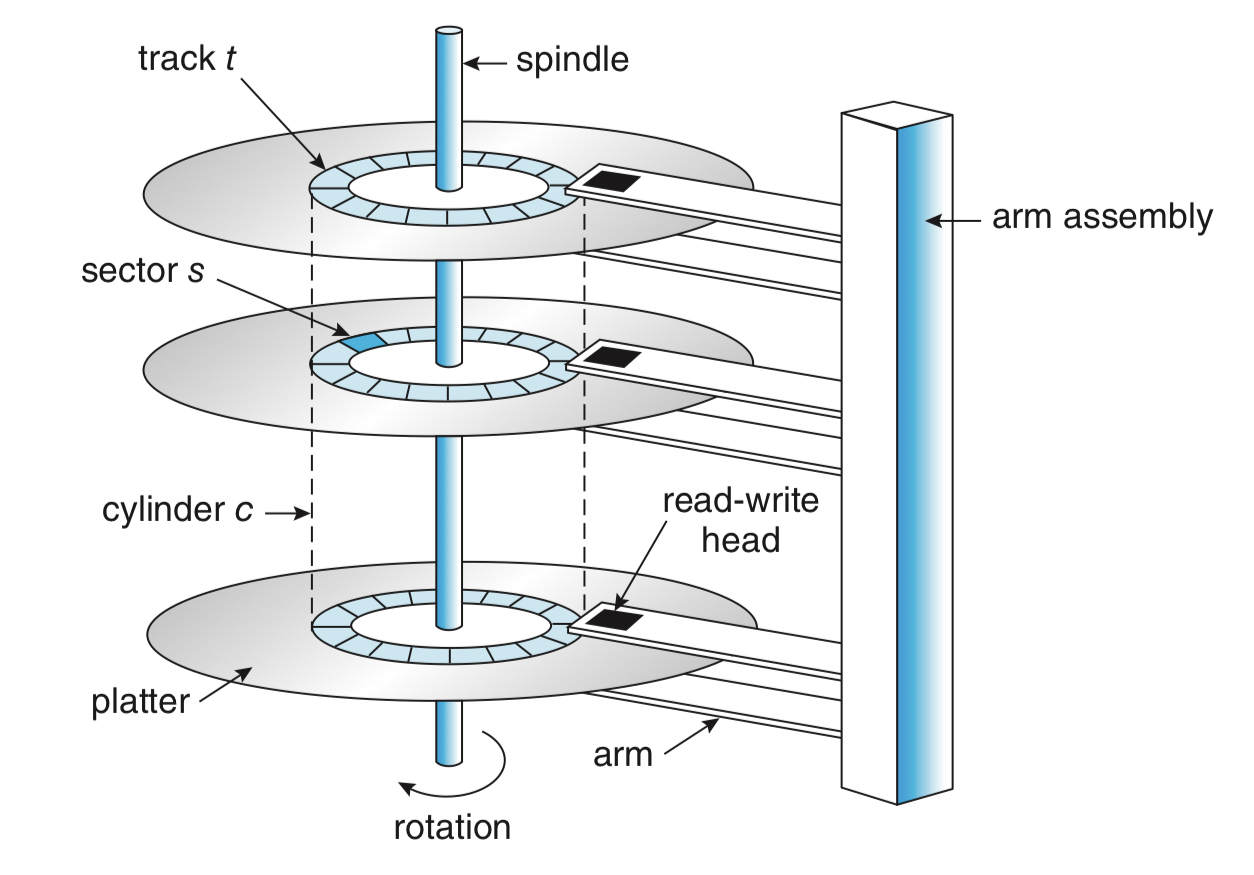
\includegraphics[width=0.7\textwidth]{figures/hdd.jpg}
            \caption{Physical structure of a HDD}
            \label{fig:hdd}
        \end{figure}
    \item \textbf{What are common HDD rotation speeds?} HDDs typically have speeds of 5,400, 7,200, 10,000, and 15,000 RPM. Some drives also power down when not in use and spin up upon receiving an I/O request.
    \item \textbf{Transfer Rate:} The transfer rate is the rate at which data flows between the drive and the computer. Typically tens to hundreds of megabytes of data per second.
    \item \textbf{Positioning Time (Random-access Time):} Consists of two parts: the time necessary to move the disk arm to the desired cylinder, called the \textbf{seek time}, and the time necessary for the desired sector to rotate to the disk head, called the \textbf{rotational latency}. Typically latencies of several milliseconds.
    \item \textbf{What are NVM devices?} Nonvolatile memory (NVM) devices are electrical rather than mechanical, like with HDDs. Such devices are typically composed of a controller and \textbf{flash} NAND die semiconductor chips, which are used to store data. Other NVM technologies exist, but are far less common. Flash based NVM devices are frequently used as disk drives (SSD), and in other instances takes the form of USB drives or a DRAM stick (RAM drive).
    \item \textbf{What are some benefits of NVM devices over HDDs?} NVM devices can be more reliable than HDDs because they have no moving parts and can be faster because they have no seek time or rotational latency. In addition, they consume less power. NVM devices are much better at random-access I/O than HDDs, since they do not need to move a physical head.
    \item \textbf{What are some drawbacks of NVM devices compared to HDDs?} NVM devices are typically more expensive and thus have less capacity than HDDs, although this is changing as time goes on. NAND semiconductors also deteriorate with every erase cycle, and after approximately 100,000 program-erase cycles the cells no longer retain data. As such NVM lifespan is not measured in years but in Drive Writes Per Day (DWPD). An NVM device near its end of life due to many erase cycles generally has much worse performance than a new device. NVM devices do not provide much of an advantage over HDDs for sequential I/O (sequential I/O is ideal for mechanical devices like HDD and tape since data to be read/written is near the head).
    \item \textbf{How is data read and written with flash memory?} NAND semiconductors can only be read and written in ``page'' increments (similar to a HDD sector). Data cannot just be overwritten, however, the NAND cells have to be explicitly erased first (and then a new write can take place). Low level: this is because electrons can only be \textit{added} to their ``charge trap'', in order to write a different amount of electrons they need to all be flushed out first. Erasure can only occur in ``block'' increments (blocks consist of several pages), and takes much more time than a read (fastest operation) or a write (slower than a read, but still much than an erase).
    \item \textbf{What makes a flash page either valid or invalid?} Imagine writing data once, and then writing an updated version of the data again later. If no block erasure has occured in the meantime, the page written to first has the old data, which is now invalid. A new page now has the current version of the data, and is valid.
    \item \textbf{How does flash memory decide where and when to write and erase blocks?} If a fully erased block exists, simply write to that block. If not, search for a block that contains only invalid pages, erase that block (erases all pages in block), and then perform the write. If there are no blocks containing only invalid pages, \textbf{garbage collection} occurs: copy valid pages in blocks to the flash \textbf{over-provisioned} area, erase the block the now unneeded block, and perform the write. Over-provisioned is simply area in the device that is always available to write to (typically 20 percent of the total).
    \item \textbf{How does flash memory try to avoid wear leveling?} Wear leveling is where blocks that are erased frequently will wear out faster than others, and consequently reducing the lifespan of the entire device. To try and wear out blocks concurrently, the device controller uses various algorithms to place data on less-erased blocks so that subsequent erases will happen on those blocks, leveling the wear across the entire device.
    \item \textbf{What are RAM drives?} RAM drives are basically sections of the system DRAM that the OS treats as a disk drive. Although DRAM is volatile, RAM drives are used because they are useful as high-speed temporary storage space. NVM devices are fast, but RAM drives are the fastest way to create, read, write, and delete files and their contents.
    \item \textbf{How do storage devices appear to the OS?} Storage devices are addressed as large one-dimensional arrays of \textbf{logical blocks}, where the logical block is the smallest unit of transfer. A logical block maps to a physical HDD sector or NAND semiconductor page. This mapping is done by the hardware. Logical block addresses are easier for algorithms used by the OS to deal with, rather than (sector, cylinder, head) or (chip, block, page) tuples. Note that this means that the OS does not deal with the intricacies of block erasures and other such details described above, this is all handled by the device controller. This also means that such storage devices are not byte addressable, it only deals in logical blocks.
    \item \textbf{Are HDDs and NVM devices the only types of storage devices?} No! There are lots of different types of storafge devices, however most are very niche. Technology is also constantly changing, meaning new types of storage devices come along.
\end{itemize}

\section*{OS Concepts 12.2: HDD Scheduling}
\addcontentsline{toc}{section}{12.2: HDD Scheduling}

\begin{itemize}
    \item \textbf{What is HDD scheduling and why is it needed?} It is the responsibility of the OS to use the hardware efficiently. For HDDs, this means minimizing acces time and maximizing data transfer bandwidth. This can be achieved by managing the order in which HDD I/O requests are serviced (basically in what order do we vist HDD block addresses?), to minimize the amount of head movement.
    \item \textbf{What approximations do HDD scheduling algorithms make?} Modern drives typically hide the intricacies of physical addresses like cylinder locations, and only expose logical block addresses (LBA; mapping of LBA to physical address done by HDD device controller). As a rough approximation, algorithms assume that increasing LBAs mean increasing physical addresses, and LBAs close together equate physical block proximity.
    \item \textbf{FCFS Scheduling} The simplest form of disk scheduling: simply perform disk I/O in the order requests come in. Wastes lots of time jumping back and forth with wild swings of the read-write head. Shown in figure \ref{fig:fcfs-disk-scheduling}.
        \begin{figure}[ht]
            \centering
            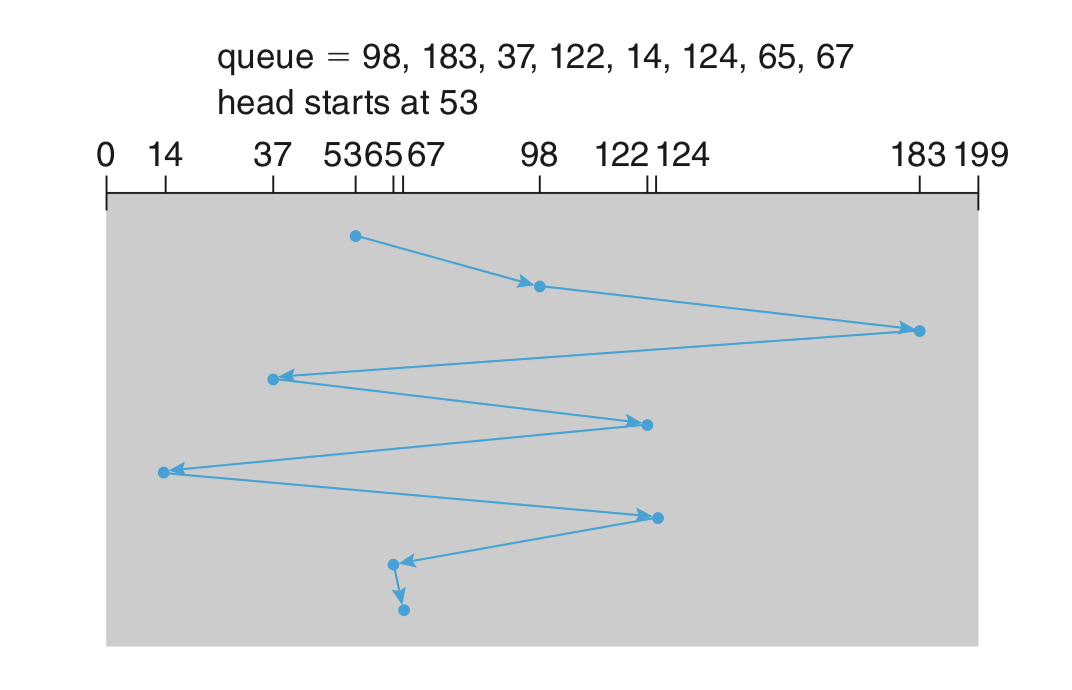
\includegraphics[width=0.6\textwidth]{figures/fcfs-disk-scheduling.jpg}
            \caption{FCFS disk scheduling}
            \label{fig:fcfs-disk-scheduling}
        \end{figure}
    \item \textbf{Shortest Seek First (SSF) Scheduling:} Service requests located in HDD cylinders closest to the current location of the head first (this results in the shortest seek for the head). Lower average response time due to minimizing arm movement, but may result in starvation for requests far away from current location of head (if new requests come in that are close to the head, the head never gets around to these far away requests). Shown in figure \ref{fig:ssf-disk-scheduling}.
        \begin{figure}[ht]
            \centering
            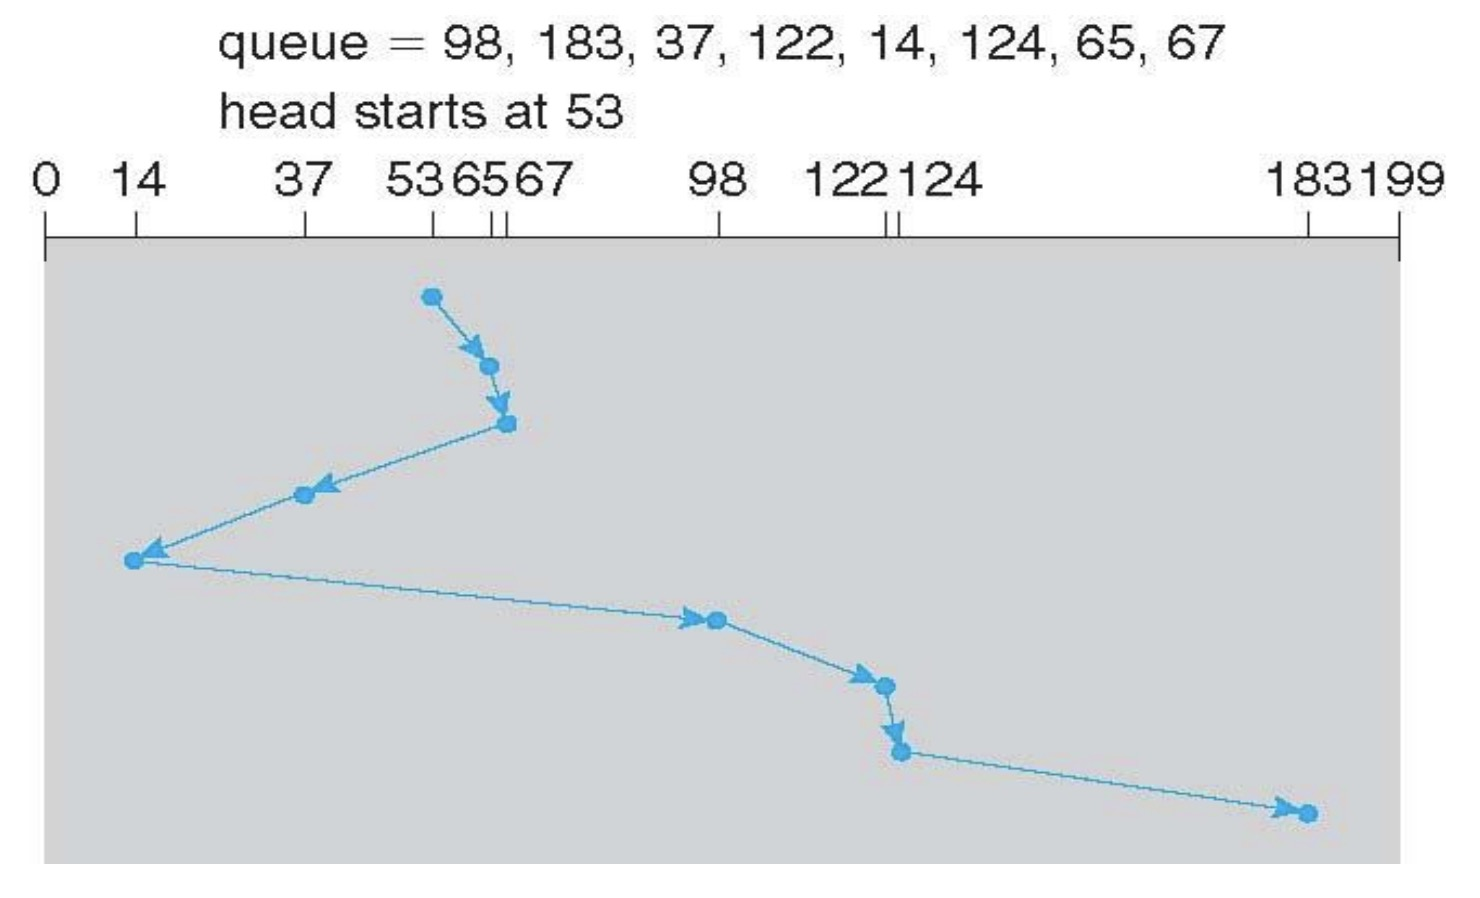
\includegraphics[width=0.6\textwidth]{figures/ssf-disk-scheduling.jpg}
            \caption{SSF disk scheduling}
            \label{fig:ssf-disk-scheduling}
        \end{figure}
    \item \textbf{SCAN Scheduling} In the SCAN algorithm, the disk arm starts at one end of the disk (an end is the first/last track in the platter), and moves towards the other end, servicing requests as it reaches each cylinder, until it gets to the other end of the disk. The direction of head movement is then reversed, and servicing continues. Shown in figure \ref{fig:scan-disk-scheduling}.
        \begin{figure}[ht]
            \centering
            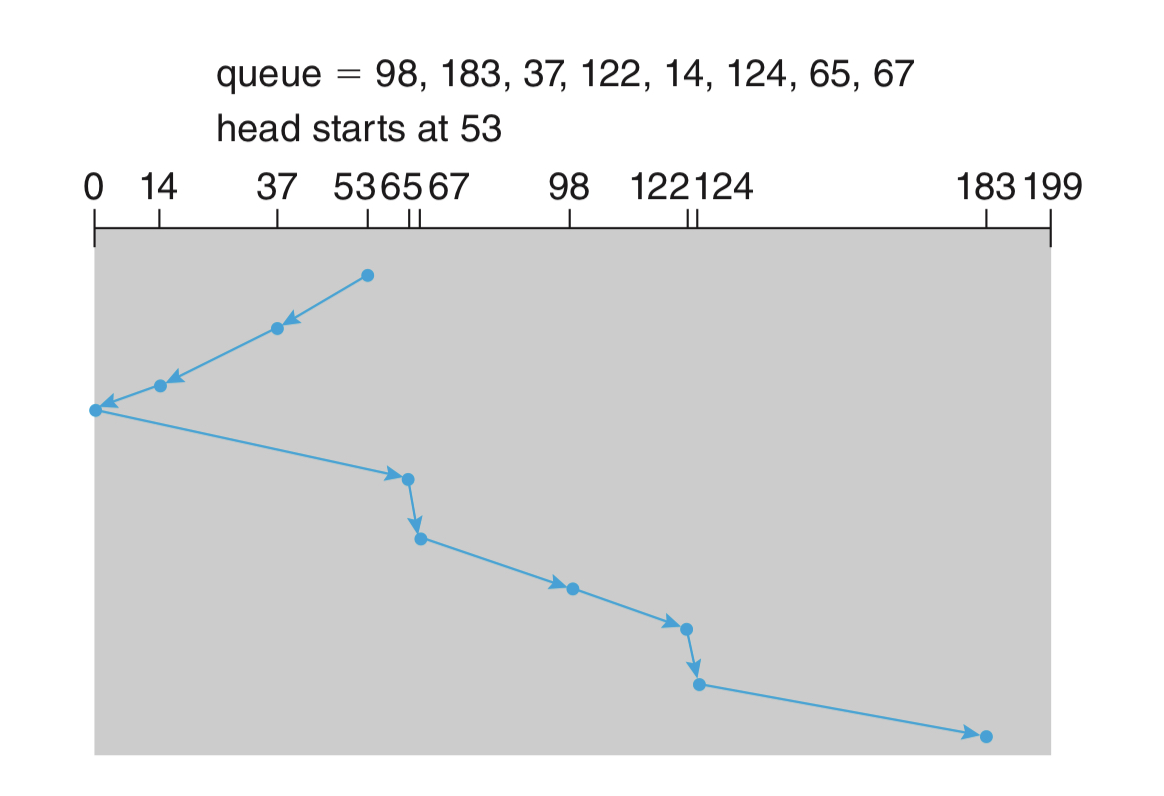
\includegraphics[width=0.6\textwidth]{figures/scan-disk-scheduling.jpg}
            \caption{SCAN disk scheduling}
            \label{fig:scan-disk-scheduling}
        \end{figure}
    \item \textbf{How are incoming disk I/O requests dealt with in SCAN?} If a request arrives in the queue just in front of the head, it will be serviced almost immediately. A request arriving just behind the head will have to wait until the arm moves to the end of the disk, reverses direction, and heads back.
    \item \textbf{C-SCAN Scheduling} With SCAN scheduling and assuming a uniform distribution of I/O requests for cylinders, when the head reaches one end and reverses direction, there will be relatively few requests immediately in front of the head, since these cylinders have already been recently serviced. The heaviest density of requests is at the other end, and lots of these requests are also the ones that have waited the longest. C-SCAN takes this into account, and instead of simply reversing direction like SCAN, when C-SCAN hits the end of the disk it simply returns immediately to the start of the disk \textit{without servicing any requests on the way back}. Essentially treats cylinders as a circular list that wraps around. Shown in figure \ref{fig:c-scan-disk-scheduling}.
        \begin{figure}[ht]
            \centering
            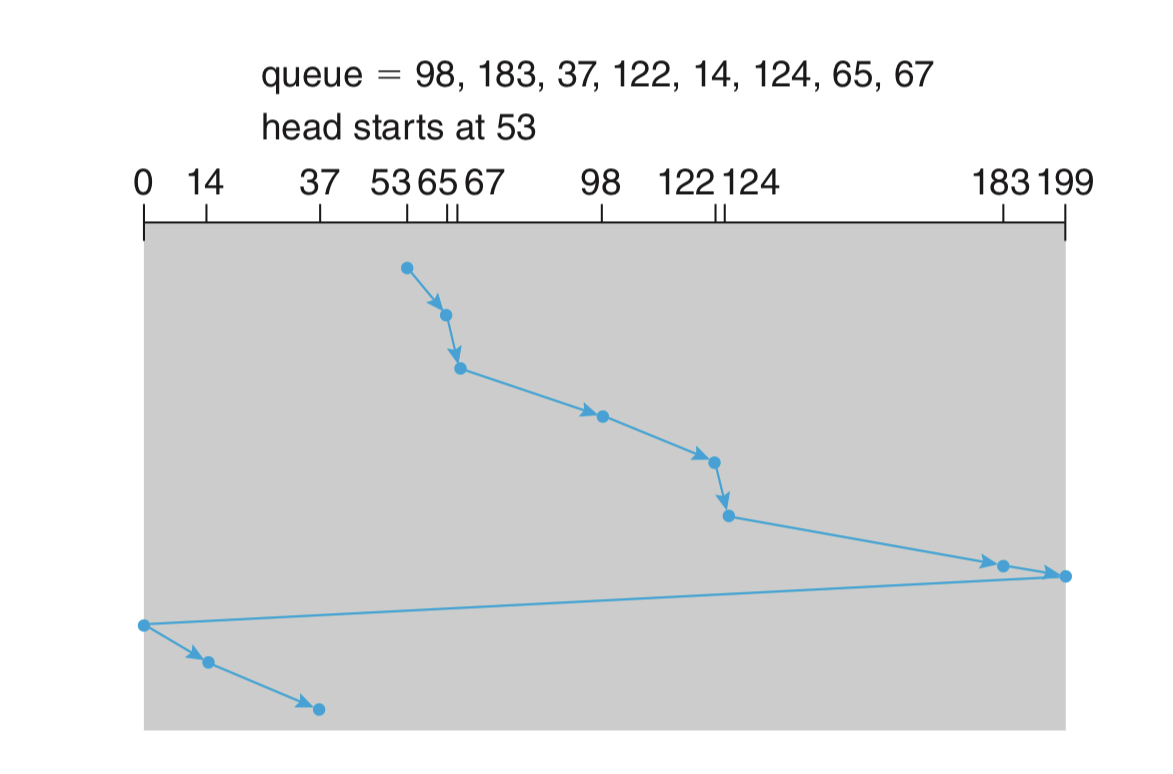
\includegraphics[width=0.6\textwidth]{figures/c-scan-disk-scheduling.jpg}
            \caption{C-SCAN disk scheduling}
            \label{fig:c-scan-disk-scheduling}
        \end{figure}
    \item \textbf{Other disk schedulers:} Other disk schedulers also exist, like the deadline scheduler, NOOP scheduler, and the Completely Fair Queueing Scheduler.
\end{itemize}

\section*{OS Concepts 11.4: Error Detection and Corection}
\addcontentsline{toc}{section}{11.4: Error Detection and Corection}

\begin{itemize}
    \item \textbf{Error Detection:} Error detection determines if a problem has occured. E.g. a bitflip in DRAM, contents of a network packet altered during transmission, or a block of data changed between when it was written and when it was read. Does not include error correction, data must be discarded.
    \item \textbf{Parity Bits:} Error detection can be done using parity bits. A parity bit records whether the number of bits in a byte set to 1 is even (parity bit = 0) or odd (parity bit = 1). If one of the bits in the byte is damaged, the parity of the byte changes and no longer matches the stored parity. The stored parity can also be damaged, in which case it also does not match the computed parity. Bitflips with an odd number of flips are detected; an even number of bitflips cannot be detected.
    \item \textbf{Error Correcting Code (ECC):} ECCs not only detect errors, but can also correct these errors. The basic idea is to send additional redundant information, from which a limited number (if too many errors, the ECC cannot perform correction) of errors can be detected and correction can be performed without retransmission.
\end{itemize}

\section*{OS Concepts 11.5: Storage Device Management}
\addcontentsline{toc}{section}{11.5: Storage Device Management}

\begin{itemize}
    \item \textbf{How does a computer boot up and start running?} When a computer is powered up or rebooted, it must have an initial program to run: this program is called the \textbf{bootstrap loader}. The bootstrap loader is very simple, and is typically located at a known address in ROM. The purpose of this program is to load other and programs (the full bootloader) which are then executed from RAM.
    \item \textbf{What happens after the bootstrap loader runs?} The next step after the bootstrap loader runs is for the full bootstrap loader to run (e.g. grub for Linux). This program is responsible for loading the operating system and transfering execution to it.
\end{itemize}

\section*{OS Concepts 12.1: I/O Overview}
\addcontentsline{toc}{section}{12.1: I/O Overview}

\begin{itemize}
    \item \textbf{Accomodating Varying I/O Devices using Device Drivers:} Hardware I/O devices are constantly evolving, and so are methods required to communicate with them. To accomodate this ever increasing variety of I/O devices, the kernel of an OS is structured to use device-driver modules. The device drivers present a uniform device-access interface to the I/O subsystem, much as syscalls provide a standard interface between the application and the OS.
\end{itemize}

\section*{OS Concepts 12.2: I/O Hardware}
\addcontentsline{toc}{section}{12.2: I/O Hardware}

\begin{itemize}
    \item \textbf{Port:} A device communicates with a computer system via a port.
    \item \textbf{Bus:} If devices share a common set of wires, the connection is called a bus. Uses a rigidly defined protocol that specifies a set of messages that can be sent on the wires. Historically called a data highway. Widely used in computer architecture and vary in signaling methods, speed, throughput, and connection methods.
    \item \textbf{Controller:}  A controller is a collection of electronics that can operate a port, a bus, or a device.
\end{itemize}

\subsection*{12.2.1: Memory-Mapped I/O}
\addcontentsline{toc}{subsection}{12.2.1: Memory-Mapped I/O}

\begin{itemize}
    \item \textbf{Processor and Device Communication:} A controller has one or more registers for data and control signals. The processor communicates with the controller by reading and writing bit patterns in these registers. I/O device control typically consists of four registers: the status, control, data-in, and data-out registers. Data registers are typically 1 to 4 bytes in size, meaning the processor needs to react quickly otherwise new data may overflow the registers and overwrite the old data. Also means I/O is basically done byte by byte.
    \item \textbf{Memory-Mapped I/O:} With memory-mapped I/O, the controller registers are mapped into the address space of the processor. The CPU executes I/O instructions using standard memory data transfer instructions to read and write the controller registers at their mapped locations in physical memory.
    \item \textbf{Memory-Mapped I/O Example:} Memory-mapped I/O for graphics. A thread sends output to the screen by writing data into the memory-mapped region. The controller then generates the screen image based on the contents of this memory. Writing millions of bytes to the graphics memory is faster than issuing millions of I/O instructions to read and write byte by byte.
\end{itemize}

\subsection*{12.2.2: Polling}
\addcontentsline{toc}{subsection}{12.2.2: Polling}

\begin{itemize}
    \item \textbf{Polling:} Polled mode I/O between a host and a controller is basically where the host has to repeatedly loop to check if the device is ready to read or write by continually checking the controller status register. Polling the controller naturally requires CPU cycles (read a device register, logical-and to extract a status bit, and branch depending on status). Polling becomes inefficient when it is attempted repeatedly yet rarely finds a device ready for service, while other useful CPU processing remains undone.
\end{itemize}

\subsection*{12.2.3: Interrupts}
\addcontentsline{toc}{subsection}{12.2.3: Interrupts}

\begin{itemize}
    \item \textbf{Purpose of Interrupts:} Interrupts are used throughout modern OS's to handle asynchronous events and to trap to supervisor-mode (kernel mode) routines.
    \item \textbf{Interrupt Handlers and OS Boot Time:} At boot time, the OS probes the hardware buses to determine what devices are present and installs the corresponding interrupt handlers into the interrupt vector.
    \item \textbf{Software Interrupts (Traps):} To get the attention of the OS, a special instruction called a trap can be executed. This instruction has an operand that identifies the desired kernel service. Library functions to issue syscalls typically implemented using traps.
    \item \textbf{Interrupt-driven I/O vs Polled I/O:} Interrupt-driven I/O is now much more common than polling, with polling being used for high-throughput I/O. Some device drivers use both: interrupts when the I/O rate is low, and switch to polling when the rate increases to the point where polling is faster and more efficient.
\end{itemize}

\subsection*{12.2.4: Direct Memory Access}
\addcontentsline{toc}{subsection}{12.2.4: Direct Memory Access}

\begin{itemize}
    \item \textbf{Direct Memory Access (DMA):} Using the expensive general purpose CPU processor to watch status bits and to feed data into a controller register one byte at a time (programmed I/O, PIO) seems wasteful. We can avoid burdening the main CPU with PIO by offloading some of this work to a special-purpose processor called a DMA controller. Essentially, DMA allows us to bypass the CPU and utilize direct memory to device I/O.
    \item \textbf{DMA High Level Implementation:} Basically, the CPU gives the DMA controller pointers to the source and destination locations and the number of bytes to be transferred. The DMA controller then proceeds to operate the memory bus directly, allowing us to perform I/O without the help of the CPU. When the entire transfer is finished, the DMA controller interrupts the CPU.
    \item \textbf{Cycle Stealing:} When the DMA controller seizes the memory bus, the CPU is momentarily prevented from accessing main memory, although it can still access data items in its caches. Although this cycle stealing can slow down CPU computation, offloading the data transfer work to a DMA controller generally improves the total system performance.
\end{itemize}

\section*{OS Concepts 12.3: Application I/O Interface}
\addcontentsline{toc}{section}{12.3: Application I/O Interface}

\begin{itemize}
    \item \textbf{Accomodating Varying I/O Devices in an OS:} The wide variety of available devices poses a problem for OS implementors (each device has its own set of capabilities, control-bit definitions, and protocols for interacting with the host). How can the OS be designed so that new devices can be attached to the computer without rewriting the OS? And when devices vary so widely, how can the OS give a convenient, uniform I/O interface to applications? Answer: by abstracting I/O hardware with device drivers.
    \item \textbf{Device Drivers:} Device drivers are kernel modules that internally are custom-tailored to specific devices but that export one of the standard OS I/O interfaces. The purpose of the device driver layer is to hide the differences among device controllers from the I/O subsystem of the kernel. Hardware manufacturers can design new devices to be compatible with existing host controller interfaces (such as SATA), or they can write device drivers for popular OS's. Each OS has its own standards for the device driver interface, so they must be ported for each OS.
    \item \textbf{Device Access Conventions:} I/O devices vary among many dimensions, such as synchronous vs asynchronous, sequential or random access, speed of operation, etc. But for the purpose of application access, many of these differences are hidden by the OS, and the devices are grouped into a few conventional types. The major access conventions include: block I/O, character-stream I/O, memory-mapped file access, and network sockets.
\end{itemize}

\subsection*{12.3.3: Clocks and Timers}
\addcontentsline{toc}{subsection}{12.3.3: Clocks and Timers}

\begin{itemize}
    \item \textbf{Programmable Interval Timer:} Most computers have hardware clocks and timers that provide three basic functions: give the current time, give the elapsed time, and set a timer to trigger operation \(X\) at time \(T\). This hardware is called a programmable interval timer. It can be set to wait a certain amount of time and then generate an interrupt, with the option of generating this interrupt periodically as well. The precision of triggers to generate interrupts is limited by the resolution of the timer, together with the overhead of maintaining virtual clocks.
    \item \textbf{Virtual Clocks:} Used to support more timer requests than the number of timer hardware channels. The kernel implements this simply by having a list of of interrupts scheduled both by the kernel and user requests, sorted in earliest-time-first order. It sets the timer for the earliest time, and when the timer interrupts, the kernel just signals the requester that the timer has gone off and reloads the timer with the next earliest interrupt time.
\end{itemize}

\subsection*{12.3.4: Nonblocking and Asynchronous I/O}
\addcontentsline{toc}{subsection}{12.3.4: Nonblocking and Asynchronous I/O}

\begin{itemize}
    \item \textbf{Blocking I/O} A blocking call causes the execution of the calling thread to be suspended (the thread is moved from the OS run queue to the wait queue). Once execution is complete, the thread is moved back to the run queue, where it is \textit{eligible} (note: eligible, scheduler decides when to run thread) to resume execution. Blocking application is easier to write than nonblocking application code.
    \item \textbf{Nonblocking I/O:} Nonblocking calls do not suspend the calling threads execution, like blocking calls do. Instead, it returns very quickly with whatever data is available (note: \textit{not} asynchronous, simply returns very quickly). One way an application writer could perform nonblocking I/O is with multithreading: some threads can perform blocking system calls, while others continue executing. Some OS's also provide nonblocking syscalls.
    \item \textbf{Asynchronous Calls:} An asynchronous call returns immediately, without waiting for I/O or whatever computation to complete (will complete at a future time, and completion is communicated to thread). The calling thread continues to execute its code. The completion of the task at some future time is then communicated to the thread (either setting some variable in the thread address space, or triggering a signal or software interrupt, or a call-back routine that is executed outside the control flow of the thread).
\end{itemize}

\subsection*{12.3.5: Vectored I/O}
\addcontentsline{toc}{subsection}{12.3.5: Vectored I/O}

\begin{itemize}
    \item \textbf{Vectored I/O:} Allows one syscall to perform multiple I/O operations involving multiple locations. This allows multiple separate buffers to have their contents transferred via one syscall, avoiding context switching and syscall overhead. Some versions also provide atomicity.
\end{itemize}

\section*{OS Concepts 12.4: Kernel I/O Subsystem}
\addcontentsline{toc}{section}{12.4: Kernel I/O Subsystem}

\subsection*{12.4.1: I/O Scheduling}
\addcontentsline{toc}{subsection}{12.4.1: I/O Scheduling}

\begin{itemize}
    \item \textbf{I/O Scheduling:} The order in which applications issue system calls rarely is the best choice. Scheduling can improve overall system performance, can share device access fairly among processes, and can reduce the average waiting time for I/O to complete. OS developers implement scheduling by maintaing a wait queue of requests for each device, rearranging the order of the queue according to a scheduling algorithm.
\end{itemize}

\subsection*{12.4.2: Buffering}
\addcontentsline{toc}{subsection}{12.4.2: Buffering}

\begin{itemize}
    \item \textbf{Buffering:} Buffering is done for three reasons. One reason is to cope with a speed mismatch between the producer and consumer of a data stream. A second use is to provide adaptations for devices that have different data transfer sizes (especially common in computer networking). A third use is to support copy semantics for application I/O.
    \item \textbf{When Buffering Can't Help:} Buffering is useful for smoothing peaks and troughs of data rate, but it can't help if on average:
        \begin{itemize}
            \item Process demand \(>\) data rate (process will spend time waiting)
            \item Data rate \(>\) capability of the system (buffers will fill and data will spill)
            \item Downside: can introduce jitter (deviation from true periodicity of a presumably periodic signal) which is bad for real-time or multimedia
        \end{itemize}
    \item \textbf{Double Buffering:} Double buffering allows decoupling of the producer of the data from the consumer, thus relaxing timing requirements between them. This works by alternating between two buffers, where the producer is writing into one and the consumer is reading from the other, and making the switch when the producer finishes writing into its buffer.
    \item \textbf{Copy Semantics:} Suppose an application has a buffer of data that it wishes to write to disk by calling the \texttt{write()} syscall. If the application modifies the buffer while the I/O is being performed, is the original or the updated data now being written? Copy semantics ensure that the version of the data is the original, the version at the time of the application syscall. A simple way to implement copy semantics is for the OS to copy application data into a kernel buffer before returning control back to the application. Despite the overhead this copying introduces, copying data from application data space to kernel buffers is common because of the useful copy semantics. Clever use of virtual memory mapping and copy-on-write page protection can also be used to implement the same effect.
\end{itemize}

\subsection*{12.4.4: Spooling}
\addcontentsline{toc}{subsection}{12.4.4: Spooling}

\begin{itemize}
    \item \textbf{Spooling:} Queue output for a device, such as a printer, that cannot accept interleaved data streams.
\end{itemize}

\section*{13.1: File Concept}
\addcontentsline{toc}{section}{13.1: File Concept}

\begin{itemize}
    \item \textbf{What is the purpose of a file system?} Without a file system, data placed in storage devices would just be one large body of data with no way of telling where one piece starts and ends. The file system provides a way to abstract away the intricacies of interacting with the physical storage hardware, and abstracts away this physical storage through the concept of logical storage units, called \textbf{files}. The file system contains two parts: a collection of files, each storing data, and a directory structure, which provides a way to organize these files.
    \item \textbf{What is a file?} A file is an abstraction of physical storage, and represents a unit of logical storage. It is a named collection of data that is recorded on a storage device. As such, it is just a sequence of bytes, of which the meaning is defined by the file's creator and user (indicated by the file type, usually in the form of an extension in the file name). Basically, a file is a name + data.
    \item \textbf{What kind of metadata is associated with a file?} Extra bookkeeping information is typically associated with a file: these are called file \textbf{attributes}. This metadata is stored separate from the actual contents of the file (usually in the directory structure). There are quite a few attributes, important ones (there are others too) include:
        \begin{itemize}
            \item \textbf{Name:} Human-readble symbolic file name.
            \item \textbf{Identifier:} Unique tag, usually a number, that identifies the file within the file system (non-human-redable name).
            \item \textbf{Location:} Pointer to a storage device and to the location of the file on that device.
            \item \textbf{Size:} Size of the file.
            \item \textbf{Protection:} Access-control information for who is allowed to read, write, execute, etc.
        \end{itemize}
    \item \textbf{What operations can be performed on files?} The OS provides several system calls to perform primitive building block operations on files. These include: creating a file, opening a file, writing to a file, reading from a file, repositioning withing a file (seek), deleting a file, and truncating a file (erase file contents but keep the attributes). Exact API is OS specific (but typically similar).
    \item \textbf{What is the point of \textit{opening} a file?} When we want to deal with a file, as a user we only the know the symbolic file name. The kernel needs to perform the [symbolic filename \(\rightarrow\) file entry] conversion, and also perform bookkeeping like checking if the file even exists, checking if the user has adequate permission for access, setting up memory buffers, etc. To avoid doing this every time when performing operations on files, the kernel provides a syscall to \textit{open} a file, which does all this once to set everything up and then returns a handle (basically a pointer) to the file. Note this means that we also have to \textit{close} our files (clean up memory buffers and other bookkeeping)!
\end{itemize}

\section*{13.2: File Access Methods}
\addcontentsline{toc}{section}{13.2: File Access Methods}

\begin{itemize}
    \item \textbf{How are the data contents of a file accessed?} Files store data, and this data must somehow be accessed and read into main memory. This data can be accessed in several ways, and OS's provide various file access methods.
    \item \textbf{Sequential Access:} The simplest access method; by far the most common. Based on a tape model for a file. A file pointer (cursor) represents location of next read or write, and is then advanced accordingly after the operation. The file pointer can be reset to the beginning, and on some systems moving it back or forth (seeking) may even be possible.
    \item \textbf{Direct Access:} Allows random access of a file. Because a file is represented as fixed-length logical blocks (abstraction of physical blocks on storage device), by providing a logical block as a parameter, direct access allows for immediate access to any block of the file. Simulating a direct-access file on a sequential-access file is inefficient and clumsy (why? idk but I think it's because of seeking overhead, not sure tho).
    \item \textbf{Indexed Access:} Built on top of direct access. Basically construct an index containing pointers to various file blocks. To find a specific record in the file, we can search (usually binary search) the index and then use the pointer to access the file directly. Shown in figure \ref{fig:indexed-file-access}.
        \begin{figure}[ht]
            \centering
            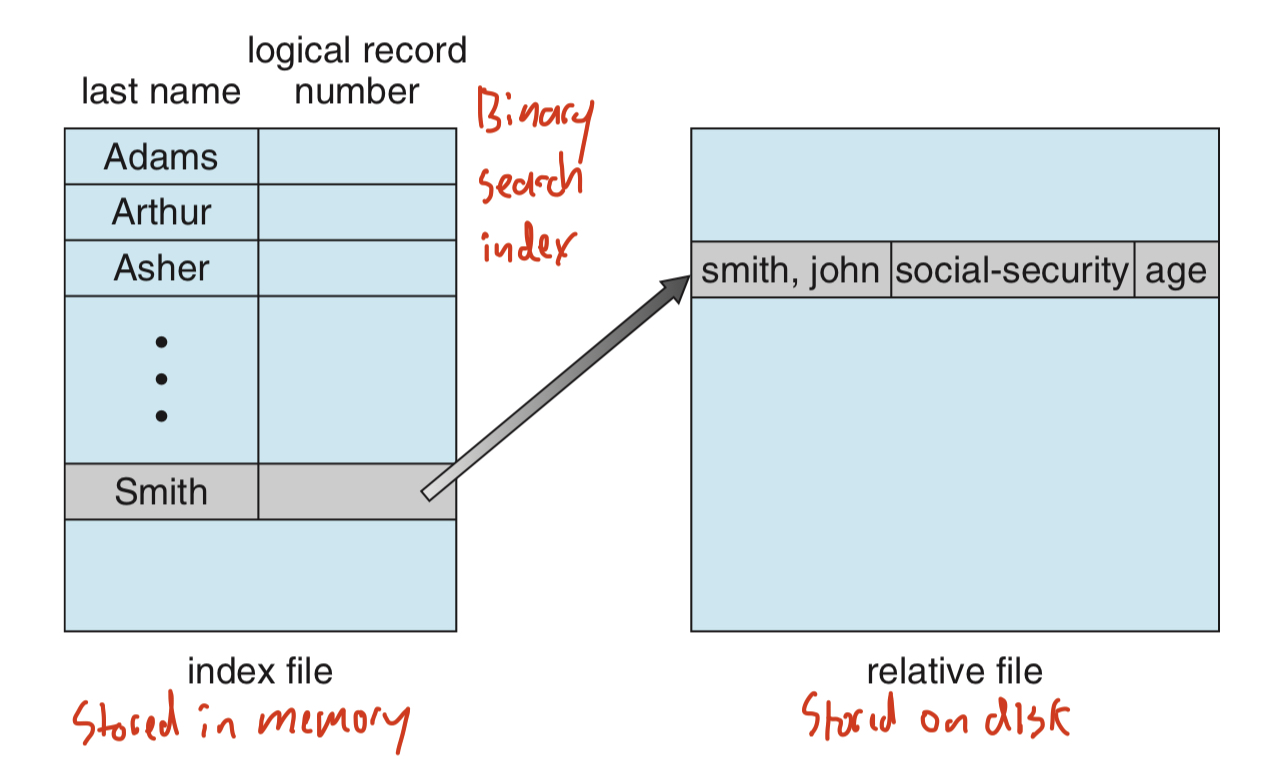
\includegraphics[width=0.6\textwidth]{figures/indexed-file-access.jpg}
            \caption{Indexed File Access}
            \label{fig:indexed-file-access}
        \end{figure}
\end{itemize}

% \vspace{4mm}

% \noindent Test here test

\end{document}
